
%********** Chapter 1 **********
\chapter{Bright Leaf: An Account of a Virginia Farm}
Henry Anderson Brumfield and his wife Julia Ann Craddock were country people who lived all of their lives in Pittsylvania County, Virginia.  Theirs was not a ``golden age'' for they lived just before and during the hard times of the Civil War and Reconstruction when Southern people had to make their own necessities and luxuries, but given good land, good health, energy and ingenuity it was possible to live well.

 

The business of their farm was raising bright tobacco.  The method was typical of most such farms in Virginia, Carolina and Kentucky at that time.  Tobacco is a demanding crop and many growers concentrated on it to the exclusion of everything else, but because Henry and Julia believed in living well they raised vegetables and fruits, pigs, beef, sheep and chickens and kept milking cows.  In their day there was no market for these extras except the few country stores or to neighbors who were apt to be over-supplied themselves.  These good things were for the family's own use.

 

They were blest with a large family of healthy children and loved them as impartially as parents ever can, and tried to treat them equally.  Like other Victorian parents they stressed dignity, reserve and respect.  Grandfather was head of his household; Grandmother was first lieutenant.  They worked as a team, reaching decisions in private and never showing divided authority before the children.  Grandfather's ``No'' was not quick and arbitrary, but when said was final unless the disappointed child could find new arguments and persuade Grandmother to present them to Grandfather.
 
 
\begin{figure}[h]
\centering
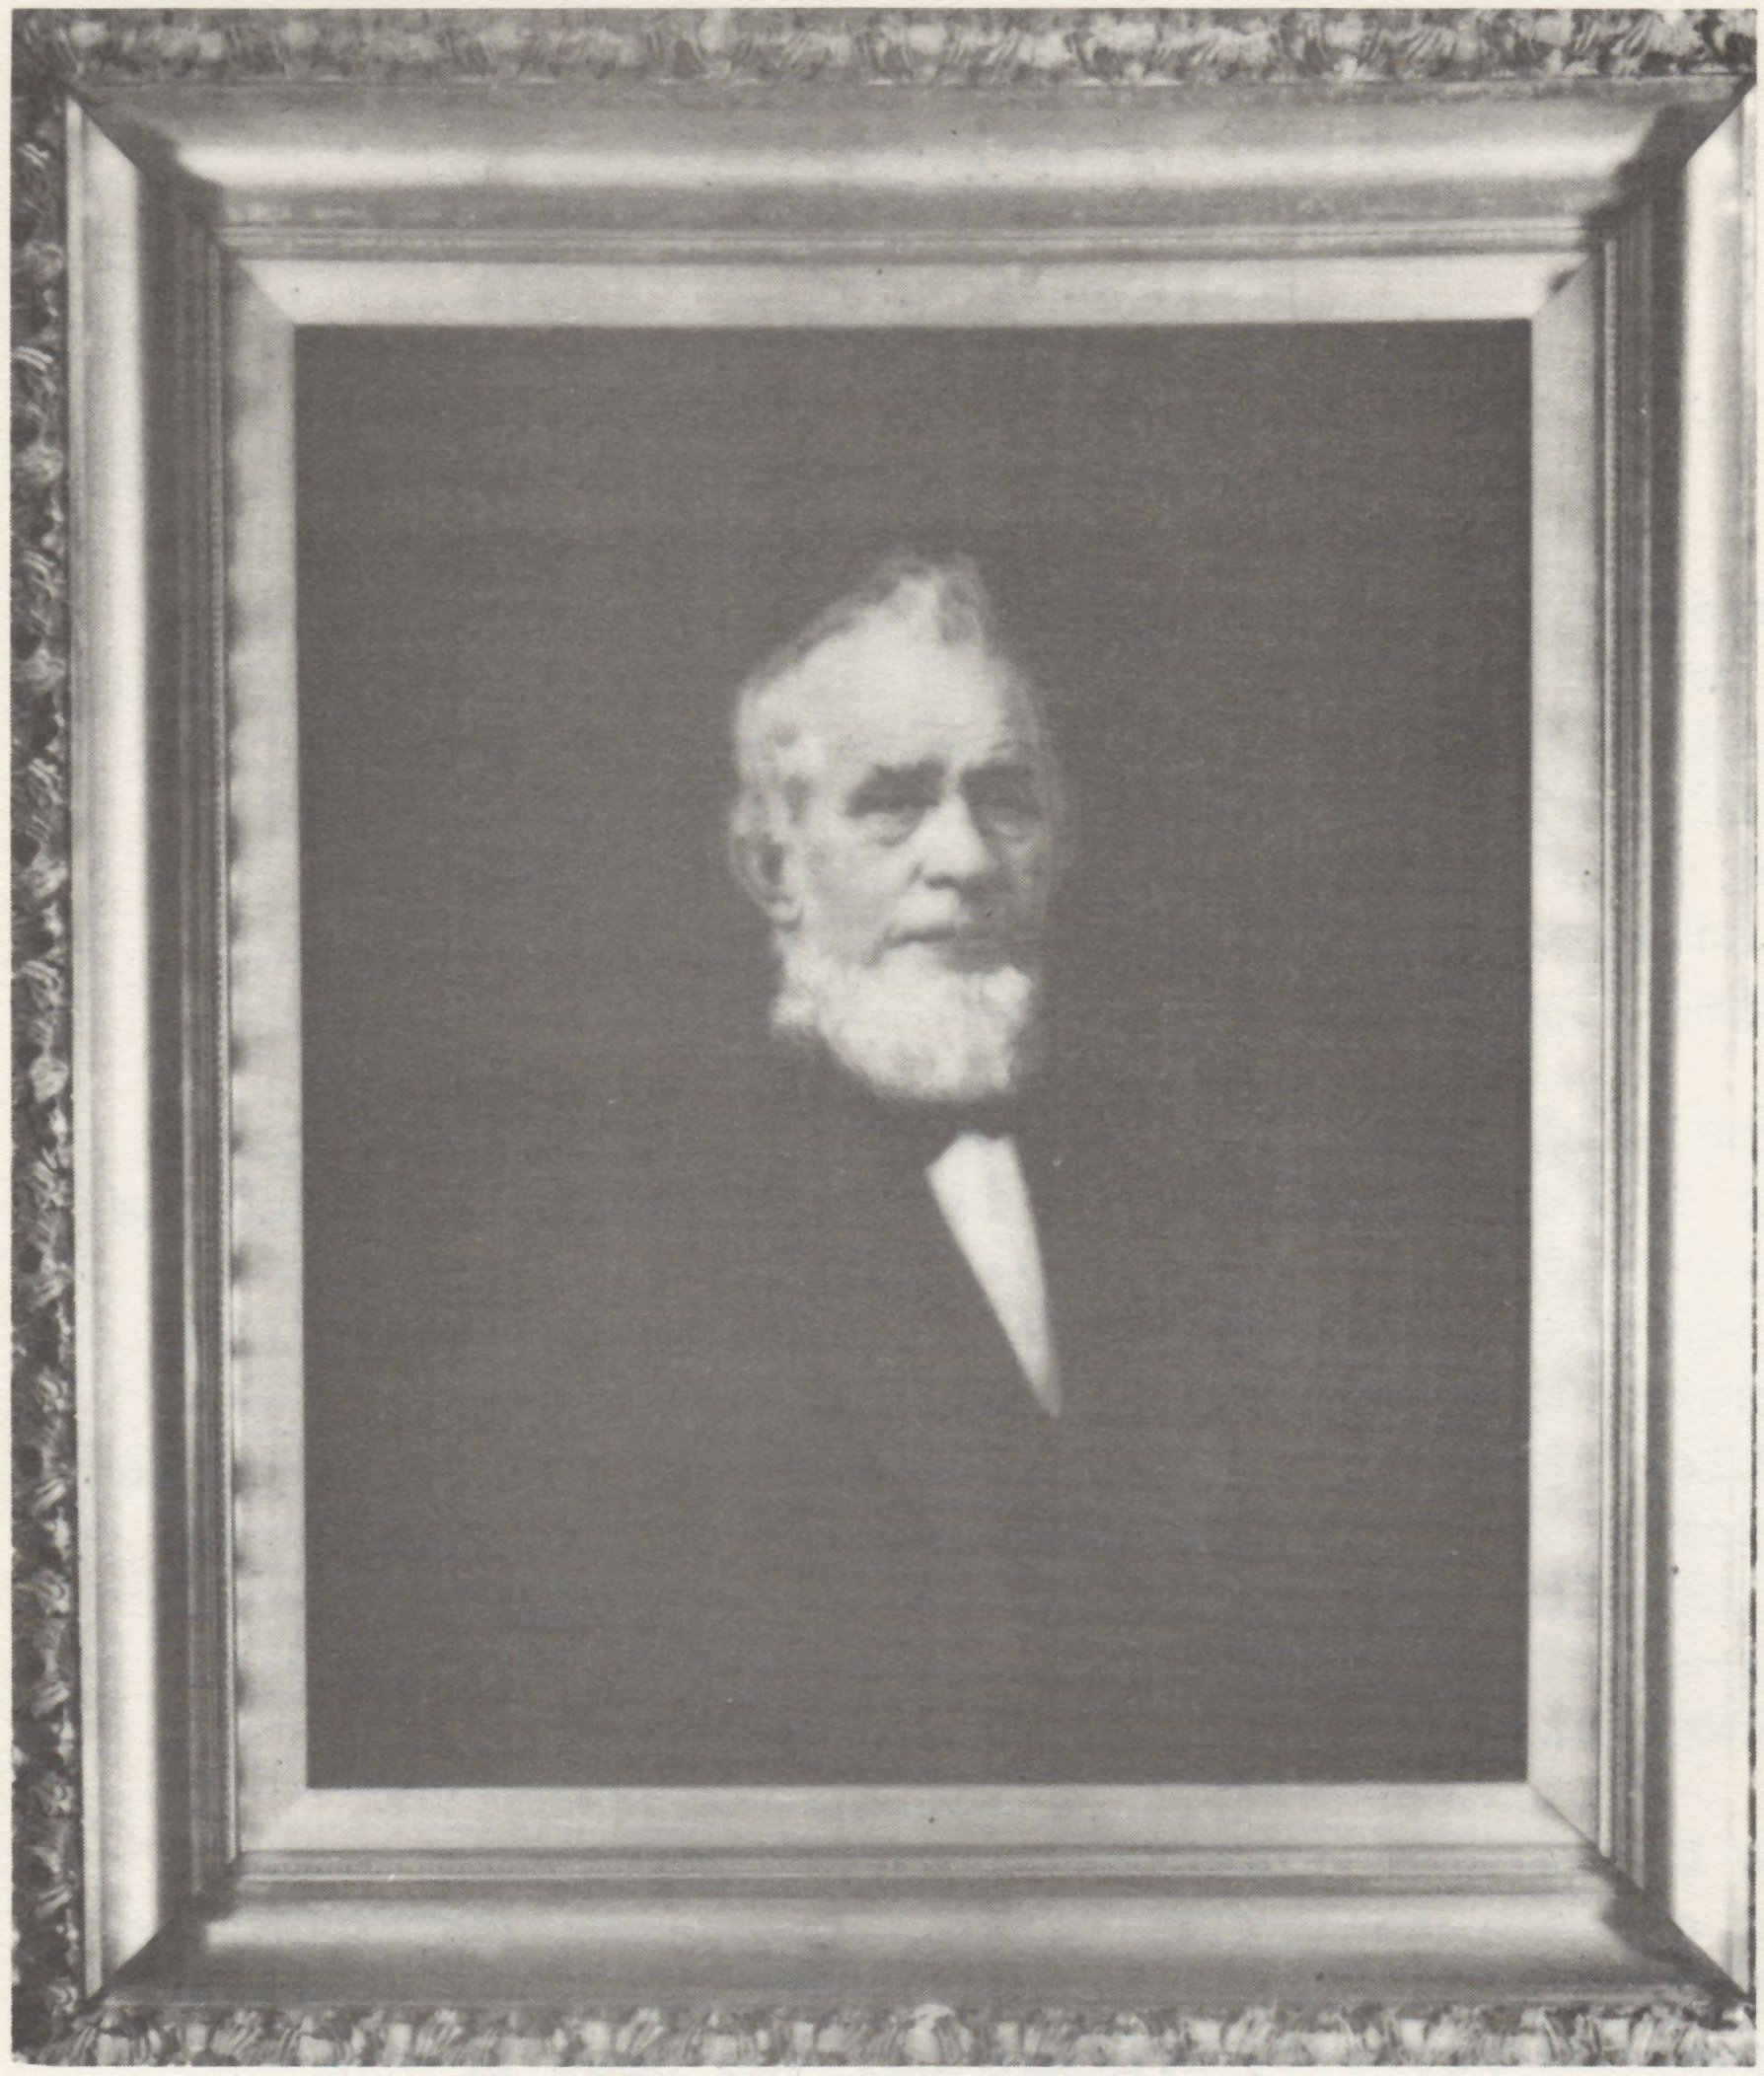
\includegraphics[width=.9\textwidth]{henry.jpg}
\end{figure}

%[Portrait of Henry]

 

Corporal punishment was expected by the children and it cleared the air and made all friendly again.  Grandmother spanked the young ones.  When an older boy needed a whipping Grandfather administered it but these sessions were largely bluff.  Henry made a big production of cutting the switch and swinging his arm back for a hard blow but the result was usually a bare flick.  He was gentle by nature and could not bare to hurt.

 
 
\begin{figure}[h]
\centering
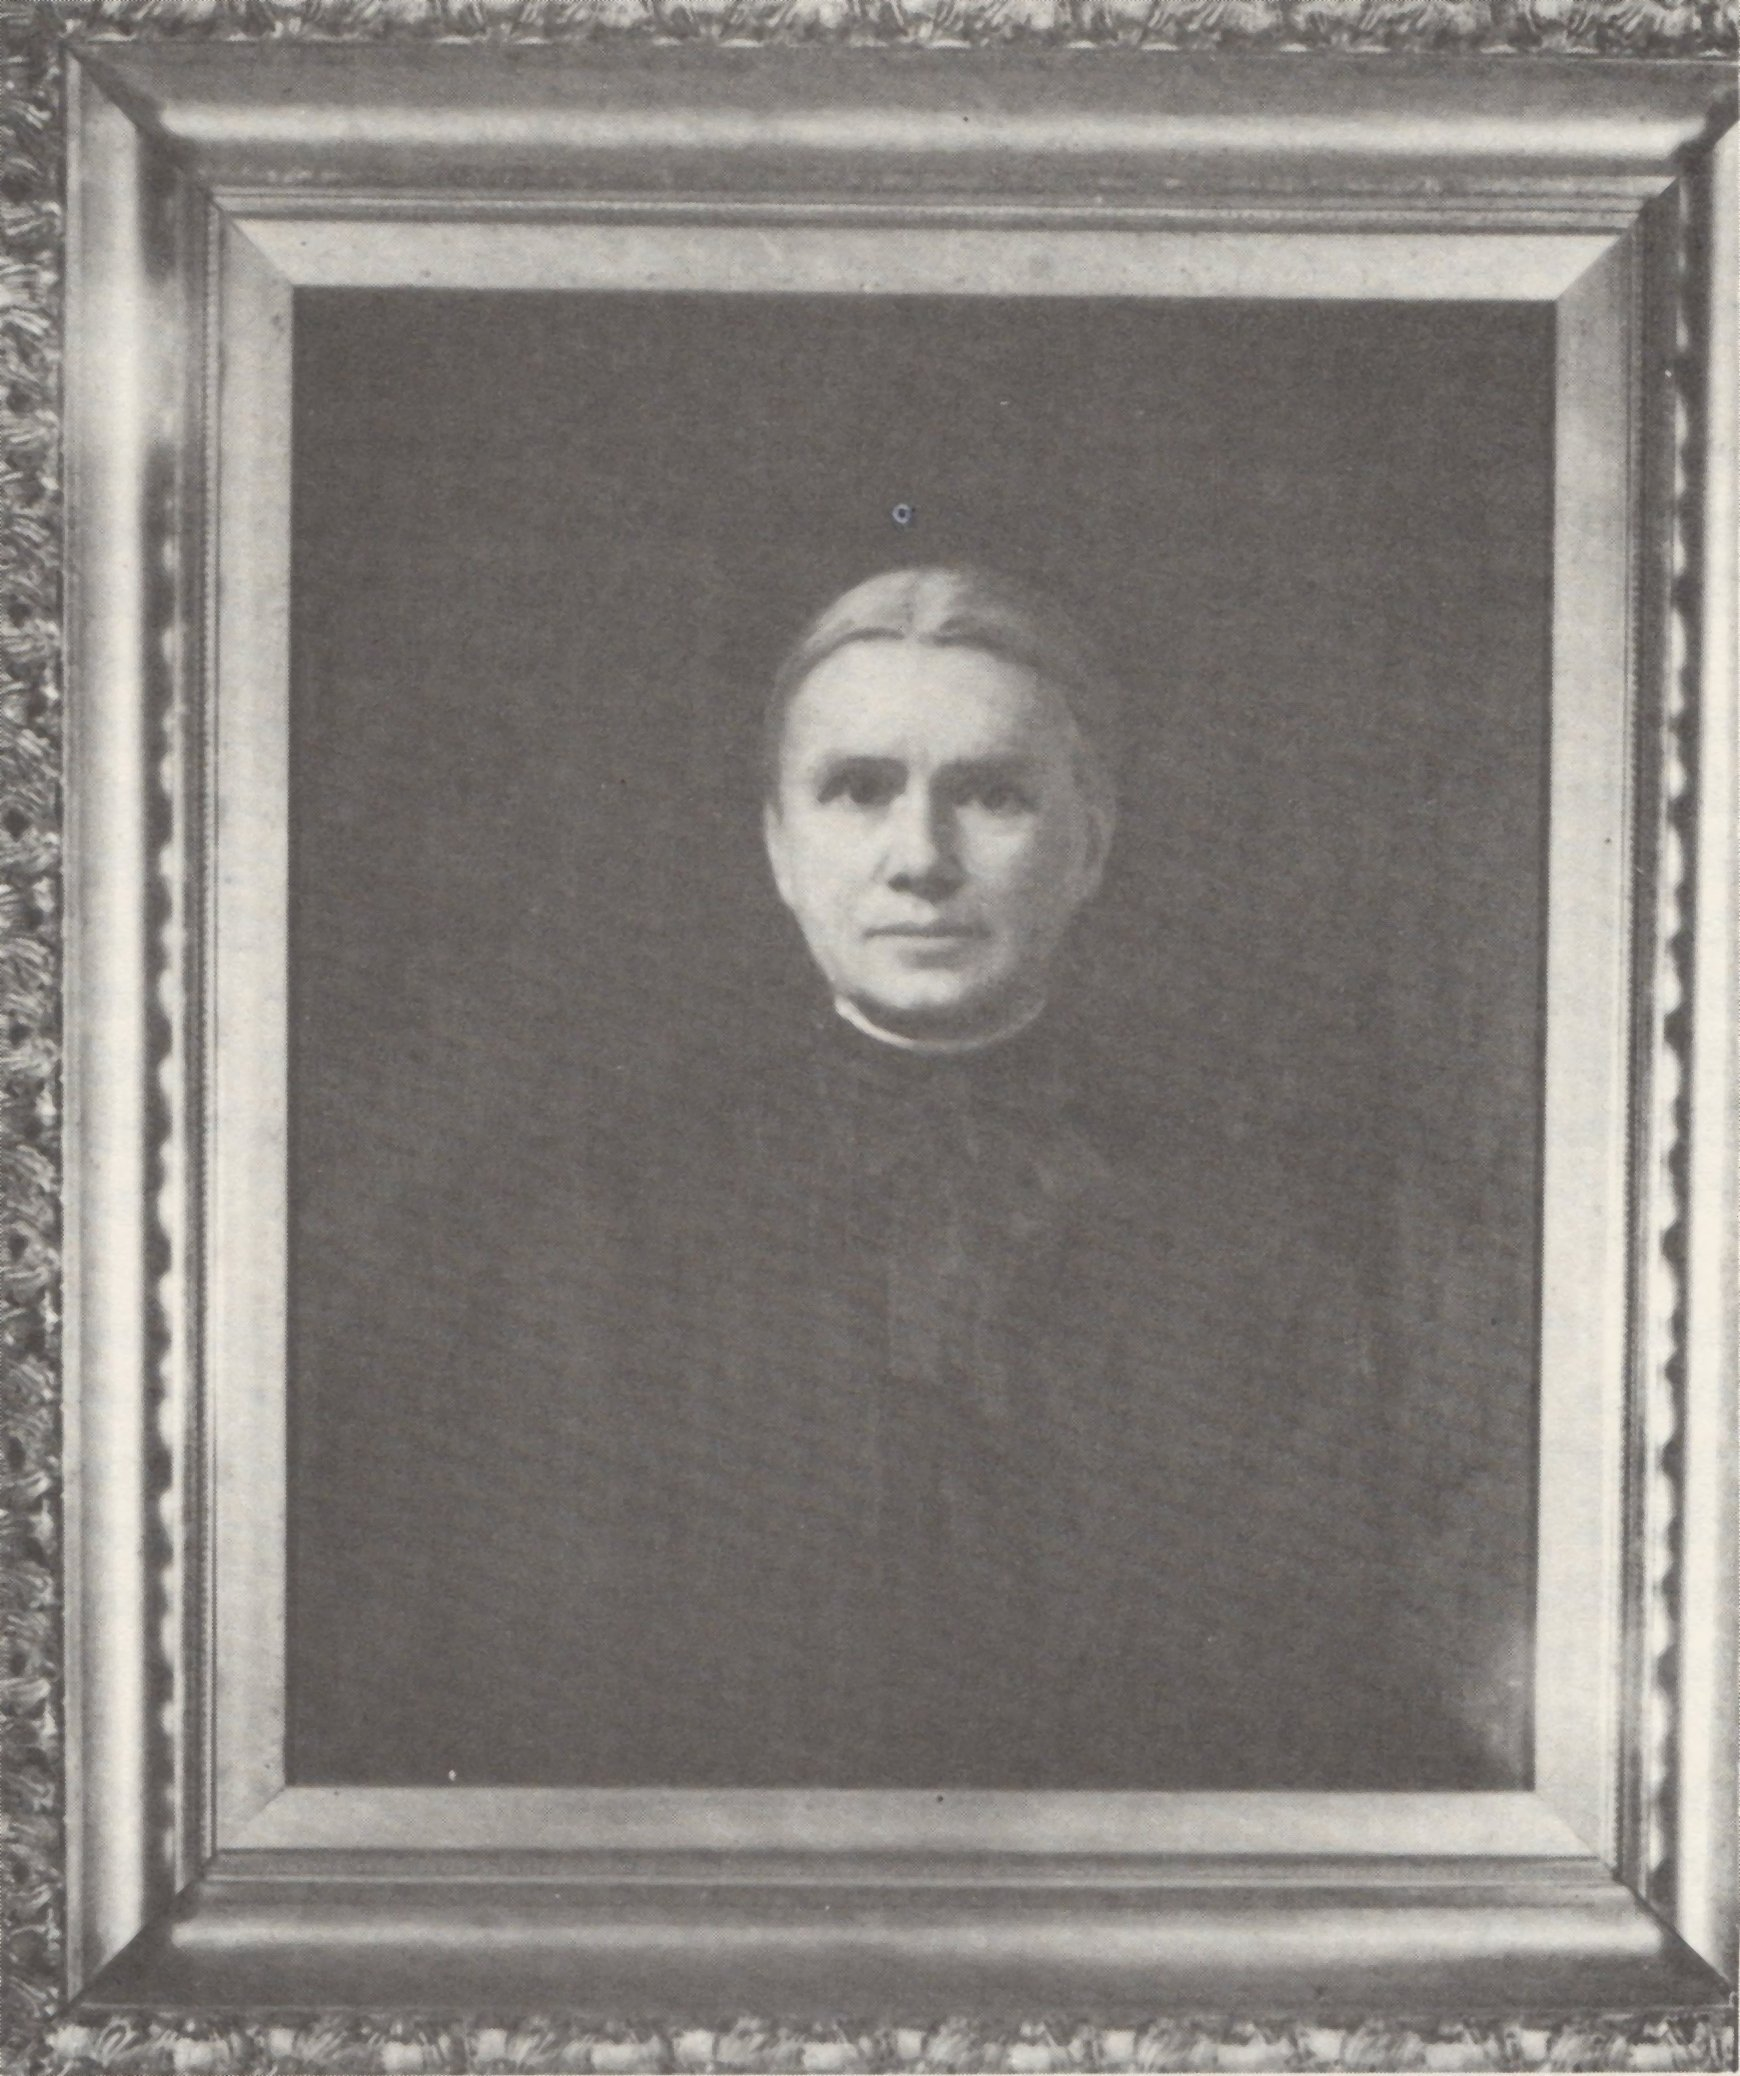
\includegraphics[width=.9\textwidth]{julia.jpg}
\end{figure}

%[Portrait of Julia]

 

Grandmother was sweet and gentle with little babies, patiently rocking them all day and night if they were sick and fretful, but when a child could walk and talk she treated him with an adult dignity.  She did not cuddle, kiss, caress or even praise him very often.  He had to merit praise before he received it and no matter how proud she was of a grandchild her praise was qualified.

 

The phrase, ``he did well for him,'' was high praise from Grandmother, who regarded vanity as a major sin and would not encourage it. This attitude plus her bossing and spanking and her quick flaring temper (which was most often directed at herself) made her appear forbidding to some of the more timid children and they said they were afraid of her.  There were many like the brave three-year-old granddaughter who boasted, ``I am not afraid of anything, not even Grandmother!''  These bold ones were flattered to be treated as grown-ups and sensed that Grandmother was really a ``softie''.  She had a sweet smile seen more often than her frown and her laugh was a quiet chuckle of genuine amusement.

 

Both parents enjoyed the company of children but did not take part in childish games.  They liked to watch children play and they listened to their talk and allowed them to tag along and learn by watching adults work.  As early as a child was able he was assigned chores of his own which he had to do before play, but plenty of playtime was left.  The boys were allowed to hunt all night if they wished so long as they turned out as usual for work in the morning.  There were sometimes stumbling, dopey workers, and once after a week of night ``possum'' hunting a son went to sleep on Friday and slept until Sunday afternoon  His mother was alarmed when she found she could not wake him.  She called the doctor who said the boy was all right only very sleepy.

 

Sometimes the boys tried horse-play or played unkind practical jokes, but these stunts were put down promptly if their parents knew about them.  Henry particularly hated quarrelling and would never tolerate teasing or picking � on those younger or more vulnerable.  On the whole members of the family were good-natured and kind with a sense of humor.  Theirs was a happy home and a pleasant place to live and visit.

 

There are many persons now living who knew Henry and Julia Brumfield and their farm.  The writer's purpose is to collect and record some of their recollections and combine them with information from diaries and old letters to give an idea of what their lives were like.  The descriptions of the Renan farm cover a span of about forty years and no great effort has been made to keep them in chronological order.  All the things described were there at one time but not at the same time.  The writer has tried to present an over-all picture that is true.

 
 
\begin{figure}[b]
\centering
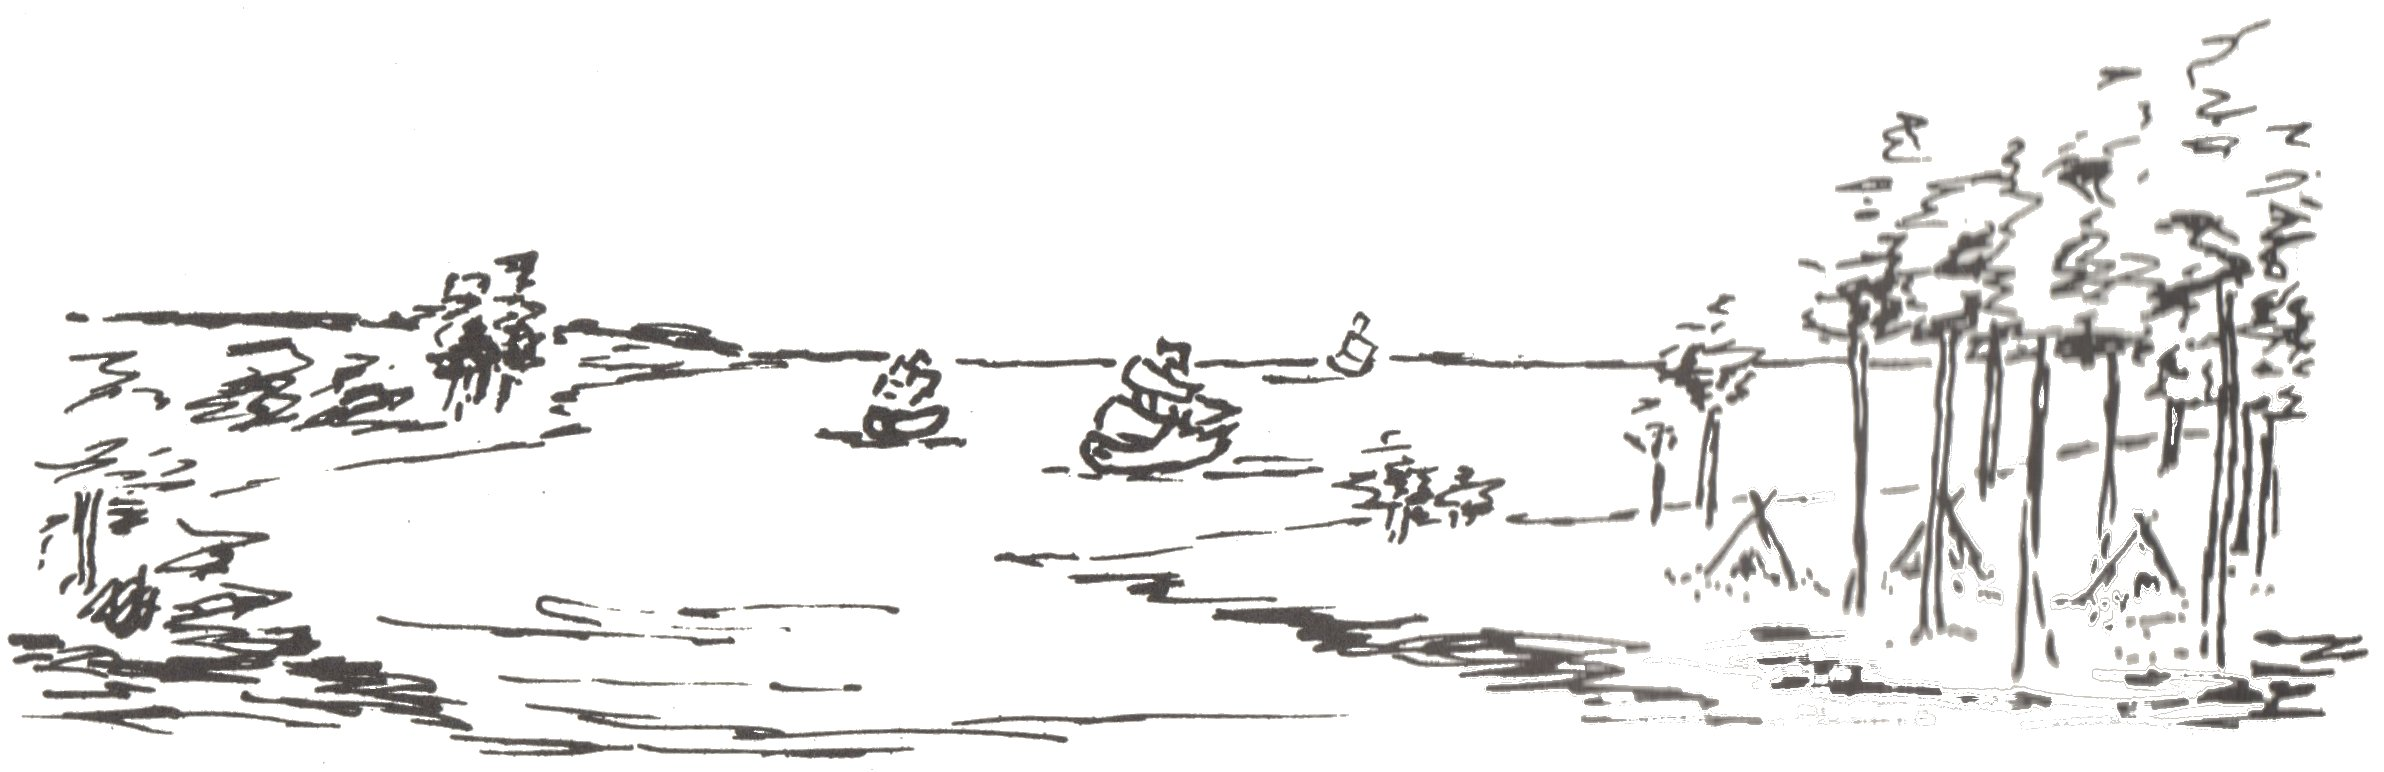
\includegraphics[width=.9\textwidth]{three_ships.jpg}
\end{figure}

%[Sketch of three ships sailing into an inlet]

 

 

\section{Forebears}

 

Ancestors of Henry Anderson Brumfield and Julia Ann Cradock were among the early settlers of Virginia.  The names BRUMFIELD, CRADDOCK, KEELING, MAYHEW, and GRUBB are found on lists of emigrants from England in Colonial times.  In the old country they worked as carpenters, masons, blacksmiths and millers.  Perhaps some were farmers although owners of English farms were not as ready to migrate as land-hungry people of the crowded cities and towns.  These families had general mechanical ability in varying degrees.  Some of the Craddocks were lawyers, clerks and professional soldiers; Brumfields and Grubbs were millers and farmers, Keelings had big plantations and slaves.  People of these names may have sailed together, and are known to have lived near together in several counties in Tidewater Virginia before they came to Pittsylvania County in the late 1700's and early 1800's.
 

The name MAYHEW is not found on the usual lists of early settlers of eastern Virginia counties, but early records of Bedford County, just north of Pittsylvania County, have many of this name.  It is thought the Mayhews came to Virginia from the north, having landed in New England.  The first deed recorded in Pittsylvania County by one of this name was in 1793.  An Henry Mayhew bought land on Georges Creek near Gretna.

 

\section{The Brumfields}
The first land purchase by a Brumfield in Pittsylvania County is recorded in the deed book on July 18, 1803.  Major Brumfield (Major is a given name, not a title) of Halifax County bought two hundred and thirty acres on Cherrystone Creek near Chatham.  This land had a grist mill on it.  Joshua Brumfield signed the deed as a witness, and it is assumed but not yet proven that Joshua was Major's son and that he lived on this land.  On February 10, 1804 Joshua Brumfield married Susannah Keeling of Halifax County.  There are references to Joshua in Pittsylvania County record books over the next few years, then he was killed in the War of 1812.  he left Susannah property in Pittsylvania County and five small children.  The eldest of these was Thomas Keeling Brumfield, the father of Henry Anderson Brumfield.

After Joshua's death his mother apprenticed Thomas to a man named Akers, to learn what trade is not known, but it may have been general farming or grist-mill operation.  The boy resented being ``bound out'' since his mother had property, including a grist-mill, but it must be remembered that no matter how much land a widow owned she had a hard time making a living. It took a man's strength to make the land produce.  Moreover a boy needs male guidance.  Thomas realized this when he was older and there was no estrangement between mother and son.
\vspace{1em}

\begin{tabular}{lllll}
\multicolumn{2}{l}{
Children of Thomas Keeling Brumfield
}&
\multicolumn{2}{l}{
Children of Henry Towler and
}\\ 
\multicolumn{2}{l}{
and Saluda Mayhew Brumfield
}&
\multicolumn{2}{l}{
and Sarah Crider Towler
}\\ 
\multicolumn{5}{l}{}\\
Elizabeth Jane &b Mar.23,1828
&
\textasteriskcentered John Winburn &b May 16,1834
\\ 
Joshua F. &b Mar.23 1829
&
Nancy S. C. &b Nov.10,1835
\\ 
Sary N. &b Aug.14,1831
&
Mary Jane &b Feb.2,1837
\\ 
Henry Anderson &b Jan.12,1833
&
Joseph J. &b Aug.17,1838
\\ 
\textasteriskcentered  Susannah &b Oct.10,1835
&
Frances &b Apr.7,1840
\\ 
Thomas N &b Dec.23,1837
&
Samuel &b Oct.25,1841
\\ 
Mary C. &b Dec.18,1840
&
Christine N. &b Aug.8,1843
\\ 
Nancy R. &b Mar.2,1844
&
Henry C. &b Mar.6,1845
\\ 
\multicolumn{5}{l}{}\\
\multicolumn{5}{c}{
Children of Thomas Keeling and Sarah Crider Brumfield
}
\\ 
\multicolumn{5}{c}{
Andrew T. b Oct.22,1847
}
\\
\multicolumn{5}{c}{
William D. b Aug.1,1851
}
\\
\multicolumn{5}{c}{
\textasteriskcentered These two were married to each other on January 8, 1857.
}
\end{tabular}

\vspace{1em}

% Following paragraph originally preceded chart
On June 21, 1827 Thomas Keeling Brumfield and Saluda Mayhew were married.  According to a family story the groom had one dollar and twenty-five cents in his pocket after he bought his marriage license.  When the Civil War broke out he owned thirteen hundred acres of land and twenty slaves and was head of a household of twenty members.  When Saluda died he was left with eight children, the youngest being only eighteen months old.  In the general neighborhood lived Sarah Towler, a widow who also had eight children, hers being between the ages of thirteen and two years old.  These two were married on February 23, 1847, combining their large families and their property.  When their own two sons were born they were a family of two parents and eighteen children and all are said to have lived in harmony.  In those days many children were wanted.  Their work was needed on the farm and children were a couple's security for old age.  Besides with neighbors so few and far away a large family furnished companionship.

\section{Henry Anderson Brumfield}

 

Henry Anderson Brumfield was born on January 12, 1833.  He could be called a blonde since his eyes were blue, although his hair was rather dark when he had grown up.  He was small in stature, but strong and wiry.  He had the usual schooling of his day which was very little.  His real school was his father's farm where he learned many things, particularly how to grow tobacco and how to take responsibility.  He was good in arithmetic.  When he was a small boy he learned the multiplication tables ``inside out and skipping about'' in less than a week.  Later he could stump the teacher on hard problems.

 

His slight build helped him get a job as a mailman when he was eighteen.  He then weighed only about a hundred pounds.  Mail was carried on horseback and the mailman had to be light in weight so as not to over load the horse.  This was before the days of Rural Free Delivery (which was not started until 1896).  His duty must have been to collect the mail at railroad stops or stage coach inns and carry it to the country post offices.  At that time some groups of householders employed a private man to bring mail to their doors, and he may have done this also.

 

Henry's interest in growing tobacco made him curious about what became of it when it left the farm, so he found work for a little while in a tobacco factory.  The most lasting thing he learned there was to make his own chewing tobacco.  Chewing tobacco was a habit he never gave up.  He knew this was bad but like other users of tobacco he enjoyed it, and could not in fairness scold his children for using the weed too.  However he would have understood the shock, years later, of his twelve-year-old son at discovering his adorable three-year-old sister chewing tobacco ``tailings'' which she had secreted in her little blue checked apron pocket.  The boy persuaded her to throw her supply away and he made a solemn pact with the little girl: if she would stop using tobacco he would too.  He kept this promise faithfully until he was grown, when he became a chain smoker of cigarettes.

 

From boyhood Henry wanted to own a tobacco farm and he saved his money for this purpose.  He told his children that the first fifty-cent piece he ever earned went into land.  He earned this coin as a very young boy by selling sheep's wool he had gleaned from bushes and briars in the pastures.  He was a saver of money, but he was not a miser.  He saved to buy good things he wanted for himself and his family.  He thought this spending was right if the money was in hand and the purchase carefully considered.  He looked upon debt with abhorrence.  Some of his descendants got the first part of this principle but missed the most important part.  One son stayed in debt, never very deeply nor did he keep the same debt very long, for he paid up often enough to keep his credit good.  However, to him a cancelled bank note meant he could borrow again.  His growing family had many delightful advantages a wiser attitude would not have allowed, and good luck and good health let him get by with it, but his parents were often fearful and ashamed for him.

 

By the time of the Civil War Henry Anderson Brumfield owned a farm near Chatham and was well established in his life's work.  Everything was disrupted by the war.

 
 
\begin{figure}[h]
\centering
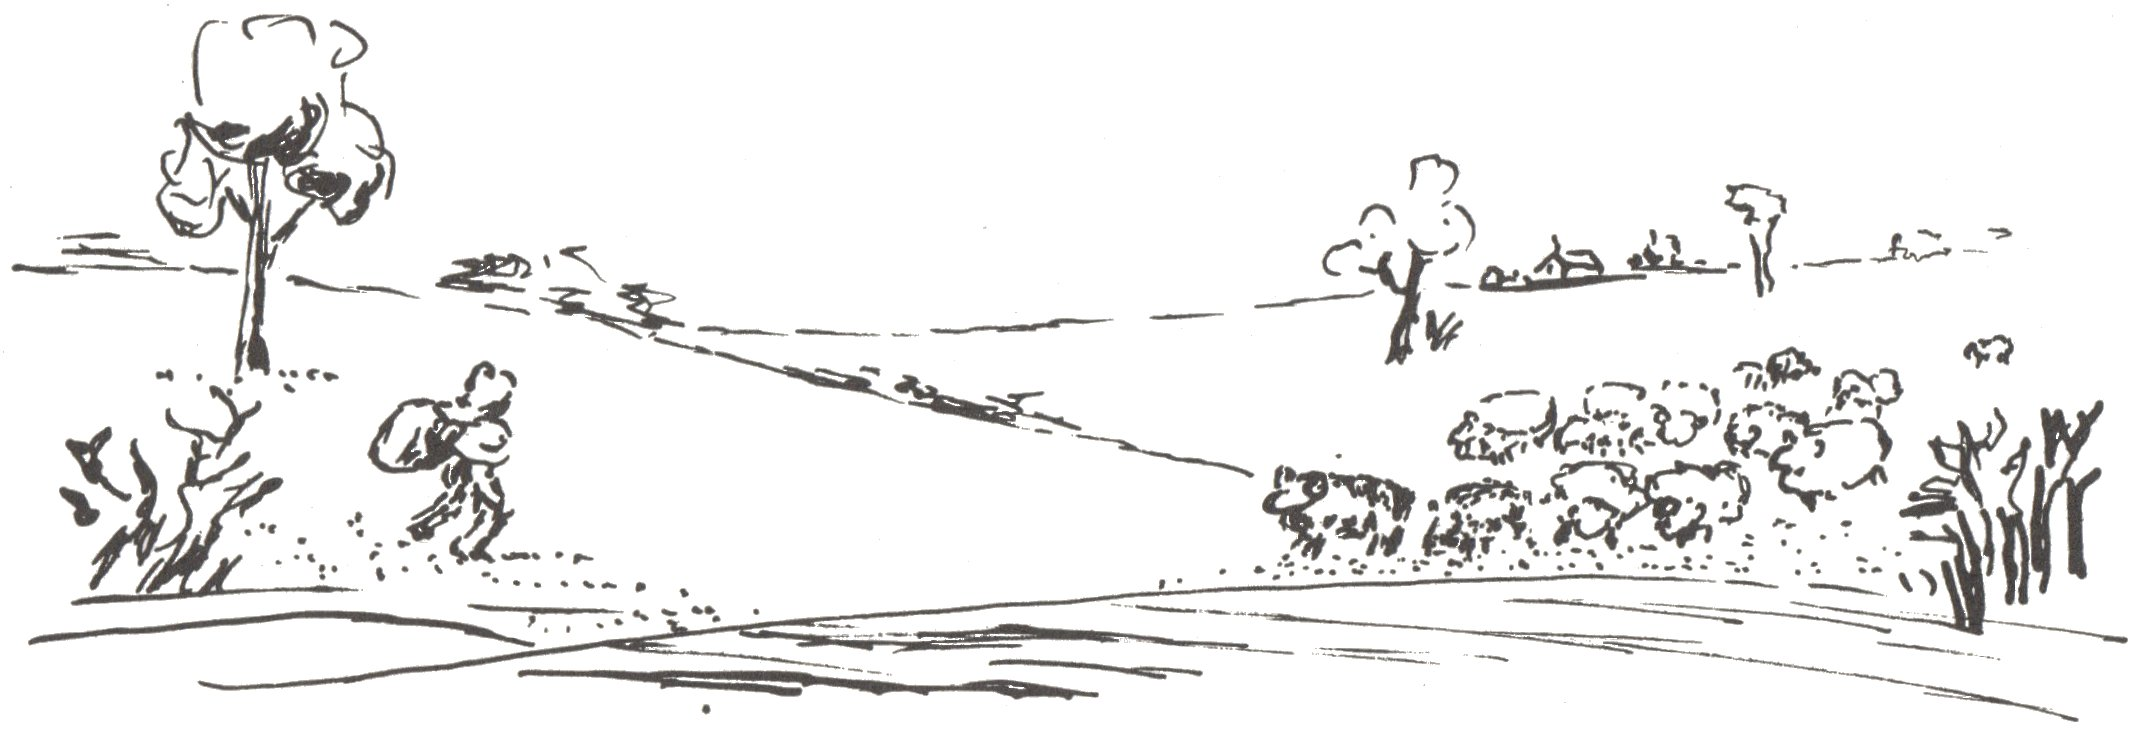
\includegraphics[width=.9\textwidth]{boy_with_backpack.jpg}
\end{figure}

%[Sketch of boy with pack on his back, among fields]
 

 

 

 
\section*{War Service}

 

In 1861 Henry and his two full brothers and three of his step-brothers all volunteered for service in the Confederate Army.  Thomas Brumfield invited everyone in the neighborhood to dinner on his grounds as a farewell party for his six sons.  Besides other foods that were served a large iron pot of stew was cooked outdoors.  The young men told of seeing their father stirring this stew with a long spoon and turning his head to keep his tears from falling into it.  This was a loving family and Brumfields were loving people who usually posed as phlegmatic.  Such a display of emotion would be long remembered.  The father's dread may have been a foreboding for two of the young men did not survived the war, and a third returned as a cripple.

 

Henry was placed in Pickett's Division, General Wise's Brigade, Colonel Watson's Command, Company C, 37th Regiment.  He served as a private for the duration of the war, and was present at some of the outstanding battles.  In 1862 he went with the army to South Carolina; he was at the Battle of Seven Pines where his brother, Thomas, was killed; at Petersburg when the Crater was blown; at the Battle of the Wilderness where he held General Lee's horse while the General went to reconnoiter.  At White Sulphur Springs he marched all night in the rain with a new case of measles and this left him with a cough and bad throat which bothered him the rest of his life.  He was often cold, hungry, unshaven and in rags.  One time he appeared at home on an unexpected leave and his father did not recognize the dirty, shaggy tramp as his son.

 

Henry never had a battle wound.  This was luck, of course, but it was also partly due to his prudence.  He and his brother Joshua were together at Petersburg.  They knew there was a sniper about, so Henry got down into a ditch and advised Joshua to do likewise.  Josh said,

            ``It's muddy down there.''

            ``Better muddy than bloody,'' was Henry's reply

Just then Joshua was shot in the leg.  The leg was amputated but Joshua recovered his health and got about with a wooden leg.  After the war he farmed in Illinois and Virginia and was married three times and had six children.

 

The above story shows that Henry Brumfield was cautious.  He was by no means timid, for all his life he liked to try new things.  At the same time he was not reckless and usually had an alternate plan ready to shift to in case his first course had to be abandoned.

 

 
\begin{figure}[h]
\centering
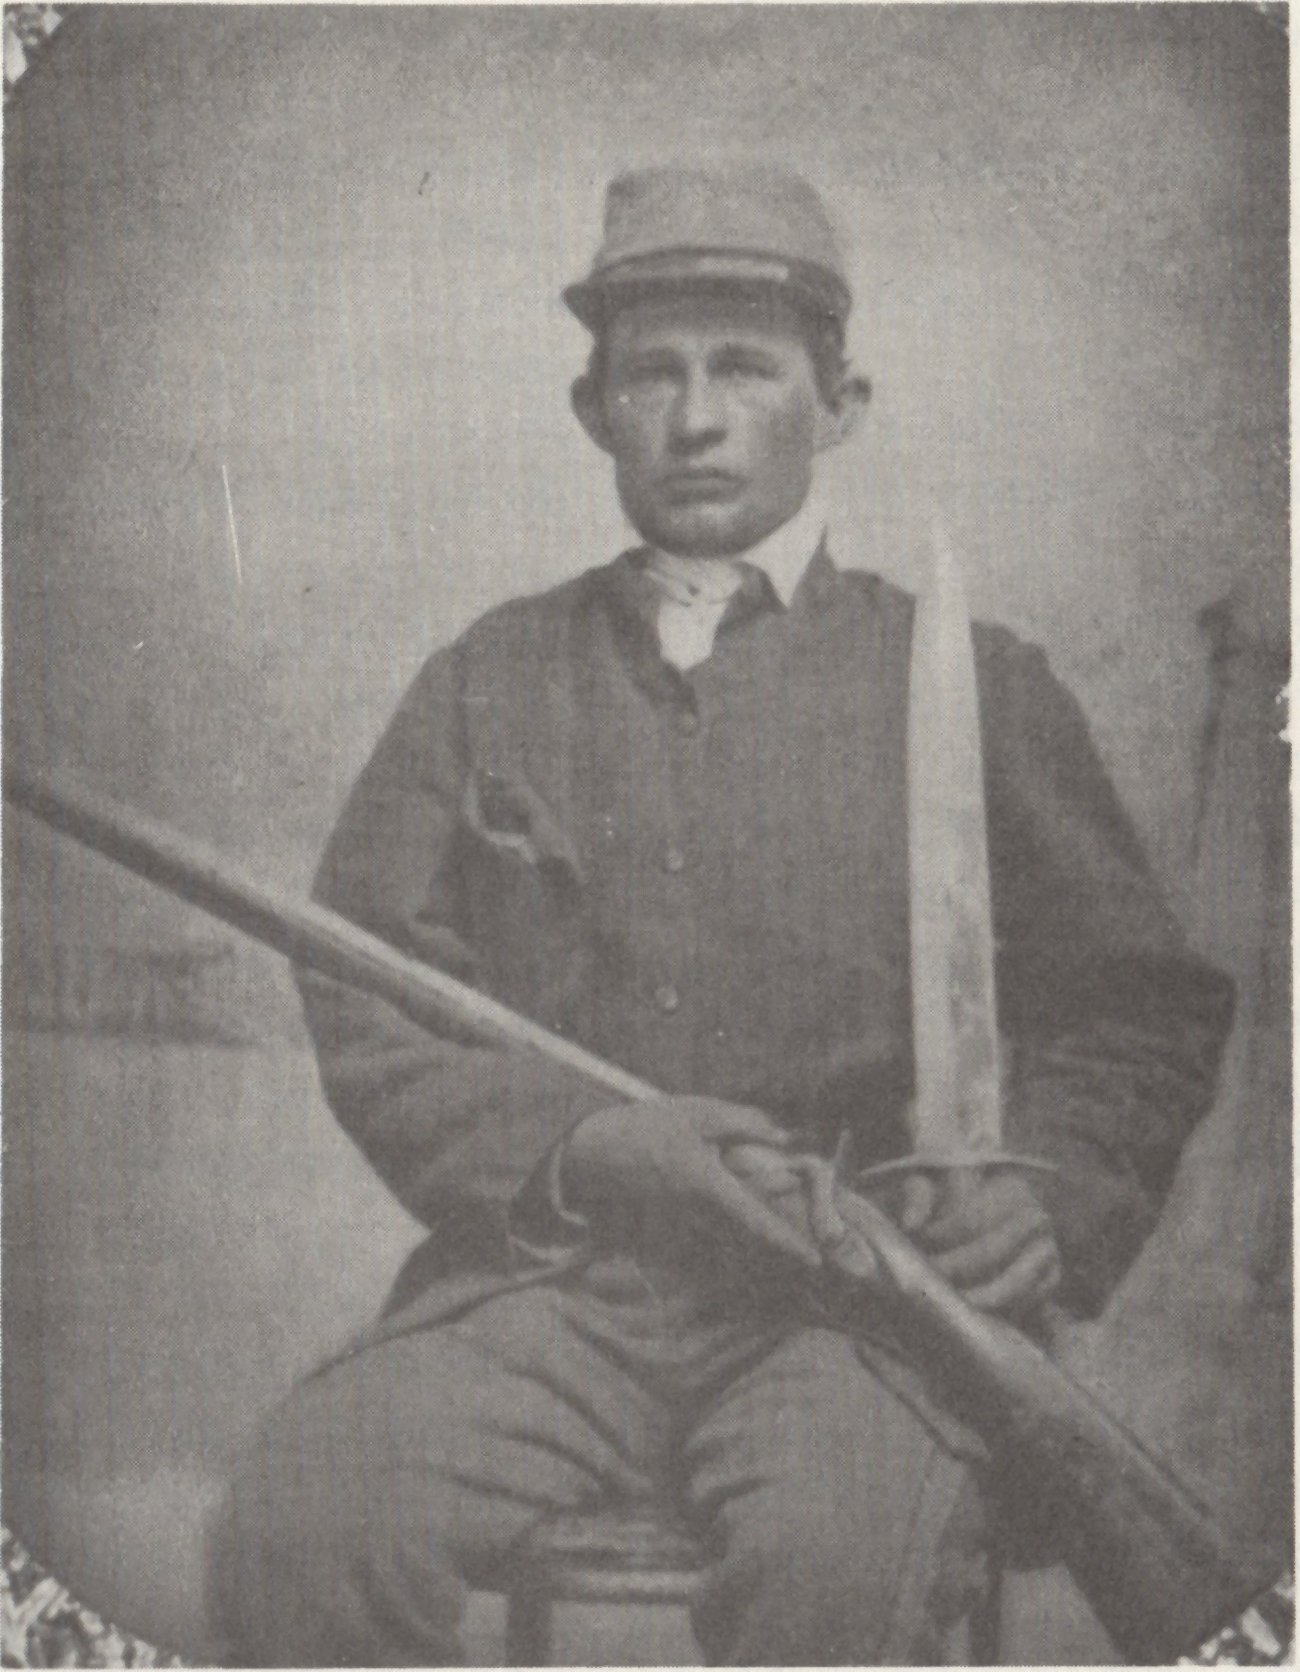
\includegraphics[width=.9\textwidth]{henry_uniform.jpg}
\end{figure}

 

Henry Anderson Brumfield in Confederate Uniform

 

In February of 1865 this soldier got a furlough and went home to marry Julia Ann Craddock.

 

 
\section{The Craddocks}

 

Craddocks lived in Pittsylvania County before the Brumfields did.  The name is listed there on the Virginia State Census records for the years 1782, 1784, and 1785.  Julia Ann's father was John Smith Craddock and her grandfather was Samuel Craddock.  Her mother was Ardena Grubb, daughter of Jesse I. Grubb.  A year or so after the young Craddocks were married, Ardena's father gave them a tract of land next to his own.  The deed reserved to him the right to build his mill dam higher, showing that the Grubbs were interested in water power just as the Brumfields were.  There is still a place known as Grubbs Mill near Chatham.

 

 

 

 

From a Craddock family Bible:
\nopagebreak
\vspace{2em}

\noindent John S. Craddock was born on August 11, 1817 and died in September 1898.
\linebreak
\indent He was married on December 6, 1842 to Nancy Ardena Grubb who was
\linebreak
\indent \indent Born November 19, 1826 and died December 1902

\vspace{2em}

\begin{tabular}{ll}
Julia Ann Frances&b October 22, 1846\\
Joab W.&b June 11, 1848\\
Mary Christine&b April 29, 1852\\
John David&b October 21, 1858\\
Charles Letcher&b February 16, 1863\\
Nancy Ardena&b November 20, 1866\\
\end{tabular}

 

 

\section{Julia Ann Craddock Herself}

 

Julia Ann Craddock was of sturdy build and fairly tall (about five feet four or five inches) and she carried herself so well she appeared to be taller than she really was.  She and her husband were about the same height.  She had a round well-shaped head, thick medium brown hair which was snow white during most of her long widowhood, and still thick and white at her death at ninety-two.  Her eyes were hazel and her gaze clear and direct.

 

Julia had ability far beyond the average.  An observer was surprised at how fast and well she got things done for she never appeared to hurry.   She was rather shy and sensitive and would not push herself forward or ``show off''.  She cultivated calmness and serenity, and most of the time she achieved theses, but she had a temper.  She kept this under control but when things did not go to suit her she would break out into a sputter.  These outbursts were mostly at herself for she was never smug or self-satisifed.  When bossing was her job she did not hesitate to boss.  When her place as mother of the family had to be yielded to her daughter-in-law she felt hurt for she had enjoyed her authority as mother.  It is a tribute to the good natures of all that there was no serious friction.

 

A tenet of her religion (the Primitive Baptist) was humility in the face of Providence.  It was presumptuous of a human to make a positive statement about what he would or would not do in the future.  With some people the qualifying statement was, ``God wiling''; with Grandmother it was ``If I live and nothing happens''.  Once when she visited in town she told her hostess that one important thing she had to do was buy a doll because she had promised one to her granddaughter.  While she was packing for the trip the little girl was watching and turning over in her head a tactful way to remind her grandmother not to forget the doll.  What she said was, ``Grandma, you said if you live and nothing happens you will bring me a doll, but if you don't live it doesn't matter about the doll.''

 

Julia loved beauty and had innate good taste both in dress and house furnishings.  She was skillful at sewing and knitting.  Quilts she made show her tiny even stitches.  Her eye was so accurate she could cut the patchwork pieces to correct size and shape without a pattern, or could decorate a patch in a crazy quilt with an embroidered flower, going by a picture that was only in her mind.

 

 

As young girls Julia and her sister Mary were taught to spin and weave.  There is a sample of some linen cloth that Julia wove when she was thirteen.  It is of unbleached flax which was raised and prepared on her father's farm.  The cloth is fairly heavy, of even threads and woven in a twill pattern.  It was made into a coat for her father, and the scrap rescued from the rag-bag is a piece of the back and part of the coat tail.  This specimen of Grandmother's work has been cut into rectangles, decorated with embroidery and framed for heirlooms.  A day's quota of weaving was eight yards.  Julia did hers so fast and well she could finish early and get away to go fishing.  Fishing was her favorite pastime then and all her life.

 

Julia Ann Craddock went to the country school and learned to read and write and cipher.  When she was about fourteen she wanted to go to the new Roanoke Female Institute in Danville which is now Averett College.  Her father told her she might go and, looking forward to the day, she was packed and ready well ahead of time. The night before they were to make the twenty-odd mile trip by buggy she laid out the clothes she was to wear.  She even rolled her stockings down to the foot so that all she had to do in the morning was to put in her toe and pull them up, wasting no time at all.

 

The next morning it was raining.  It poured so hard it was foolish to think of making the trip that day over the muddy roads.  It continued to rain all the rest of the week.  When it finally stopped raining and the roads were dry enough to travel, Julia's father had changed his mind.  There was no later chance for going away to school, because the Civil War started and her parents wanted her at home.

 

 

\section{Henry and Julia}

 

Henry was thirteen years older than Julia.  By the time she was grown he was in the army.  His courting had to be done on the brief leaves a soldier is allowed, but somehow they managed to meet and fall in love.  The match was approved by both families, but they thought of a wedding sometime after the war when Julia was older.

 

All during his service Henry had sent his pay to his father to buy more land for him.  He now had considerable property.  Thinking of this and his love for Julia, Henry wrote to her father saying, ``these are parlous times'' (this phrase is remembered and quoted from his letter which is now lost).  He continued to this effect: if anything should happen to him he wanted Julia to have his land, therefore he asked permission to marry her on his next leave which was soon due.  This argument carried weight with John Craddock and he gave his consent.  Julia Ann Craddock and Henry Anderson Brumfield were married on February 21, 1865.

 

The wedding took place at the Craddock home.  No description of the bride's dress is given, but it is recorded that the groom wore a black broadcloth coat with a satin vest (which is still in existence), black homespun pants and calfskin boots.  Henry went back to join his regiment.  Six weeks later he was present at the surrender at Appomattox.  His parole was handed to him there at 1:00 P.M.  He walked home, a distance of sixty miles, arriving in time for breakfast next morning.

 

 

\section{The Migration}

 

The defeat of the Confederacy left Virginians in despair.  Many decided to leave the South and Thomas Keeling Brumfield was among them.  Most of his children and step-children agreed with him and the migration began.  The first small group of three bachelors, one Brumfield and two Towlers, left early in 1866.  They bought land at Patoka, Illinois, and were joined there later by other members of the family.

 

Thomas Keeling Brumfield and his third wife, his two youngest sons and his daughers and step-daughters who still made their homes with him, as well as some of the married ones and their families went to points in Indiana.  All Henry Brumfield's nearest relatives left the State. A few of these returned to visit and a very few came back to stay, but for the most part there was no close contact with them again.  Henry and Julia preferred to stay in Virginia.

 

 


\section{The Young Couple's First Homes}

After the surrender in April 1865 there was still time to plant and raise a crop.  Henry did this on his father-in-law's land, but both he and his wife wanted to be on their own.  Early in 1866 they to moved Henry's farm on Bearskin Creek near Chatham, a farm of about three hundred and sixty acres.  They moved into a little old log cabin which had only two rooms and a loft.  The floor of the lean-to kitchen was the bare earth.  Julia found keeping a clean house almost impossible, and it was trying for her, for her standards were high.

Shortly before the war was over, when it was clear that the South would lose, Henry exchanged some of his Confederate money for greenbacks.  he did this even though he was heart-sore over the defeat and hated Yankees.  (He hated Yankees so much he would never wear the blue denim overalls which most farmers wore because the color was like the Yankee uniform.)  Defeat had to be accepted, however, and his responsibility and his love for Julia made him see the wisdom of having some Federal money to give them a start on their land.

This ready money enabled him to buy a poor horse (no good horse was left in the South), and with the help of one hired man, a Negro with the euphonious name of Beverly Hayley, he was able to make eighteen hundred dollars that year.  This was a high gross income at the time from a small farm worked by only two men.  It is so remarkable that it has been questioned since the figure is given from memory.  Henry Brumfield kept careful records, but his papers were destroyed about fifteen years after his death.  The United States Census Reports give the average price of tobacco grown in the United States in the year 1868 as a little over ten cents a pound.  \emph{Italics}{The Southern Planter}, however shows that bright leaf flue-cured tobacco sold for as much as ten times that.  This type of tobacco brought a higher price in 1867 than in 1868, and probably still more in 1866 when it was even more scarce.

\section{Henry Brumfield's Big Ambition}

Over the next few years Henry Brumfield built a good house, a stable and several barns, but all the time he was looking for land more pleasing to him.  He moved his family to a farm adjacent to the County Poor Farm, and this was their home for a number of years, but Henry had an ambition that could not be reached in this locality.  Proud of their large family and wanting them always with them, the parents thought of the future.  They could think of nothing more wonderful than to give each child a one-hundred acre farm adjoining their own when he or she married.  How nice it would be to have them all living close and working at the most satisfying work in the world!

There was not enough land for sale near there, besides Henry wanted timber as well as cleared fields and good forests were not easy to find.  He looked as far as Tidewater Virginia without success until at last he heard of land in his own Pittsylvania County about twenty miles to the northeast.  This area was known to the family as Canada-land, so named from an early setler.  It was described as backwoods where the only signs of civilization were steel traps and bowie knives.  There were virgin forests but also some homes and cleared land.  Prudent Henry bought two hundred acres there and put a tenant of his community on it.  This tenant made such a good crop that Henry was convinced the region was a good choice, and the family planned to move.

\section{The Swap}

Next to Henry Brumfield's acres in Canada-land was a house and farm owned by Mr. Jake Graves called ``Aspen Grove''.  the Graves family had lived there during the war and for a long time before (a gravestone in their family cemetery bears the date 1807), but they were ready to give it up.  Henry was eager to have it, so the two owners arranged to trade farms -- the Brumfield place on Poor House Road of two hundred and seventy-three acres for the Graves place in Canada-land of two hundred and fifty-six and three-fourths acres, Brumfield to pay five dollars to boot and Graves reserving his family cemetery.  Besides houses and land the swap included farm animals, machinery and tools and some furniture.

The families moved in 1882.  The Brumfield family consisted of the parents and eleven children, the eldest being sixteen and the youngest not quite two years old.  They made quite a cavalcade.  Kind neighbors loaned wagons and helped with the move.

 
\begin{figure}[h]
\centering
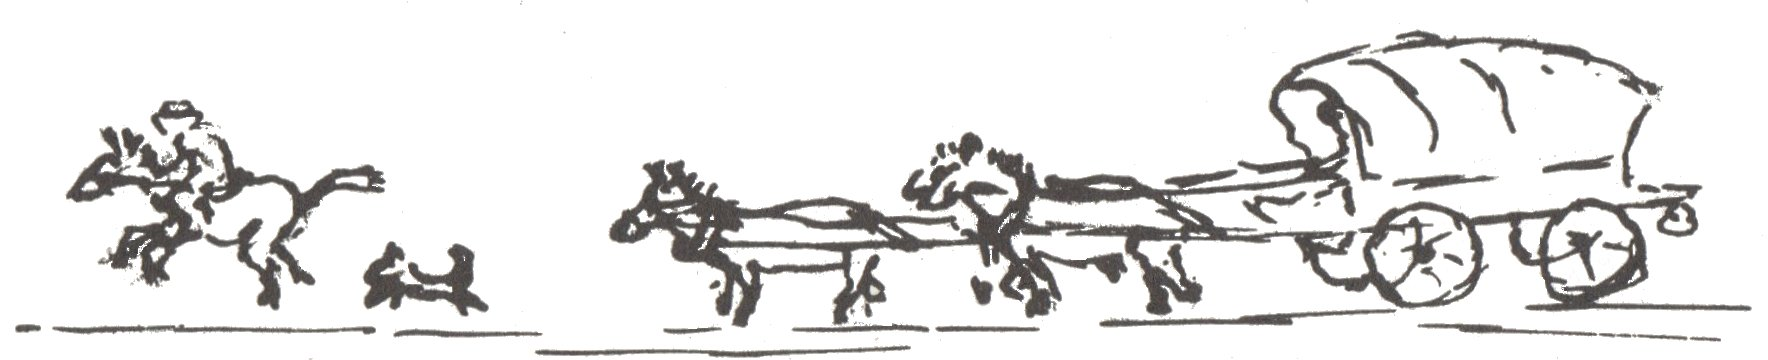
\includegraphics[width=.9\textwidth]{wagon_and_team.jpg}
\end{figure}

 

[Marginal illustration of a wagon and team of four]

 

\section{First Years in Canada-Land �� The Family Complete}

 

Planting a crop and arranging the house gave all hands plenty to do that first year (1882).  All the settling-in went well, but the next year (1883) was a time of tragedy.  The first distress was in January when the other had a severe case of pneumonia and gave birth to a boy on January twenty-fifth who died at birth.  This was the first death in the immediate family, but before the year was out there were two more.  In August there was a raging diphtheria epidemic.  Several of the Brumfield children were dangerously ill at the same time and the two youngest died.  These three little graves were the first in the family graveyard.  They set aside a square of ground on the hill west of the house, next to the Graves' plot.  Sometime later these graves were marked and the square enclosed with a white picket fence.  The cemetery now contains thirty-two graves.  The picket fence has been replaced by a post and chain enclosure, and the area is kept in good condition under the supervision of a granddaughter who lives nearby.

 

Grieving could not be indulged for busy life went on.  Soon there was a happy event to celebrate, for on November sixteenth there was the first family wedding.  The first and second daughters were engaged to cousins and both planned early weddings, perhaps a double wedding.  A death in the family of one of the young men made it necessary for the eldest daughter to postpone her wedding, so the second daughter was married first.  The wedding took place in the family parlor, and Julia purchased a Haviland china tea-set to grace the occasion.

 

The next year (1884) began with a very happy event.  On January second a little girl was born who was a life-long comfort to her mother and is and always has been a delight to all who know her.  Henry and Julia's last child, a boy, was born on November the eighth, 1887.  Julia and Henry themselves delivered him and their other children who were born after the move to Canada-land.  Julia herself bathed and dressed these babies in their first clothes.

 

A few years after the birth of their last child two more members were added to the Brumfield family.  Henry's brother, Joshua, had died leaving his third wife with one child of her own and five step-children.  Shortly afterward she remarried.  The new step-father was unwilling to provide for all these orphans.  He kept his wife's own child and the oldest boy who was fourteen and able to work on the farm, but he bundled the other four children into a buggy and without any explanation dumped them at their uncle Henry's home.  Julia and Henry took them in with love and kindness.  They made it clear to their own children that these cousins were to have as sure a place in their home as if they had been born there.  A few weeks later a maternal uncle, brother of Joshua's second wife, came and took two of his sister's children home to live with him.  The other two children stayed with the Brumfields.  The elder child, a girl, was married in the parlor there in 1897; the younger, a boy, stayed until he was grown and on his own. Both kept warm ties with the family, visiting whenever they could, and when the nephew died at age seventy-five his body was brought back for burial in the family cemetery.

 

 

 

\section{The Children}

\begin{tabular}{rllll}
1. & Saluda Ardena & b April 28, 1866 & ``Dena'' & Mrs. George Blair\\
2. & Mary Susan & b April 21, 1867 & ``Mollie'' & Mrs. Johnson Reynolds\\
3.&Nancy Elizabeth&b May 20, 1868&``Lizzie''&Mrs. Tim Bennett\\
4.&Julia Katherine&b July 9, 1869&``Kate''&Mrs. Walter Harvey\\
5.&John Thomas&b October 10, 1871&``John''&\\
6.&Charles Francis&b January 25, 1872&``Charles''&\\
7.&Henry Lee&b April 18, 1873&``Lee''&\\
8.&William Andrew&b May 26, 1875&``Will''&\\
9.&James Anderson&b April 10, 1877&``Jim''&\\
10.&Anne Sarah&b May 28, 1879&``Annie''&d August 5, 1883\\
11.&Letcher David&b May 9, 1881&&d August 6, 1883\\
12.&son&\multicolumn{3}{l}{b and d January 25, 1883}\\
13.&Carrie Ellen&b January 2, 1884&``Carrie''&Mrs. Marvin Smith\\
14.&Benjamin Franklin&b November 8, 1887&``Ben''&\\
\\
\textasteriskcentered&Sarah&b May 3, 1874&``Sarah''&Mrs. John Emerson\\
\textasteriskcentered&Henry Anderson&b January 28, 1878&``Henry''

\end{tabular} 
 
\vspace{2em}
\textasteriskcentered (Children of Joshua Brumfield)
 

 

 


\section{Building the House}

The year 1884 that began so happily with the birth of a daughter was the beginning of a period of modest prosperity.  Crops over the next two decades were good and there were money and enthusiasm for improvements.  The family's first need was for a more comfortable house, and work was begun that spring.  The family had moved into the old Graves house as it stood.  Like most old houses it had been built in stages.  There was a dilapidated old wooden part, itself built in stages with rooms poorly arranged and floors at different levels, and so old the roof shingles and floor boards were put in with wooden pegs.  This was attached to a newer three-storey section built of brick.

The contractor hired for the job was a skilled brick mason and carpenter who knew how to make his own bricks and how to dress his lumber, but he could neither read nor write.  There was no architect but Henry, Julia and the contractor worked out a practical plan tailored to the family's needs.  Since the newer brick ell was in good condition, it was kept.  The old wooden part was torn down and in its place three storeys of brick was added.  The finished house had ten rooms, if you count the pantry as a room, and three halls and two porches, all of spacious dimensions.

During the building the contractor and many other workers lived with the Brumfields.  Henry and the older boys helped with the building: Julia and the older girls were kept busy cooking for the crowd, and the mother had little time to tend her baby.  This job was assigned to the nine-year-old son, who like all the Brumfields loved small animals, especially babies.  He liked to read and while looking after the baby he could sit tailor-fashion in front of her cradle and rock and read by the hour.  The Bible was one of the few books available, and he read and reread the stories and learned long passages by heart, and he regarded this as a valuable part of his education.  By the next year when the baby was big enough to hang on he carried her piggy-back all over the farm, sometimes spelled by the next younger brother who was part of this inseparable trio.

The contractor started his job by making the bricks.  Anyone who has seen the bright red clay soil of that part of Virginia will readily concede that suitable clay was on the place.  The clay was dug, ground to a powder, worked into a mud and molded in home-made molds.  After sun-drying the bricks were reshaped a little and stacked for firing. More than one hundred and twenty-five thousand bricks were made and fired, a job that took eighty cords of wood.

The timber used for the house also came from the place.  There were thousands of original forest pines, and carefully selected trees were cut and sawn into planks.  Some of the planks were so wide window and door facings could be fashioned from one board, even where the walls were eighteen to twenty-four inches thick.

 

[BWB:Illustration of the house taken in late 1960s/early 1970s by Neil and Mary Ann Brumfield.  Negative is in their possession, somewhere.]

 
\begin{figure}[h]
\centering
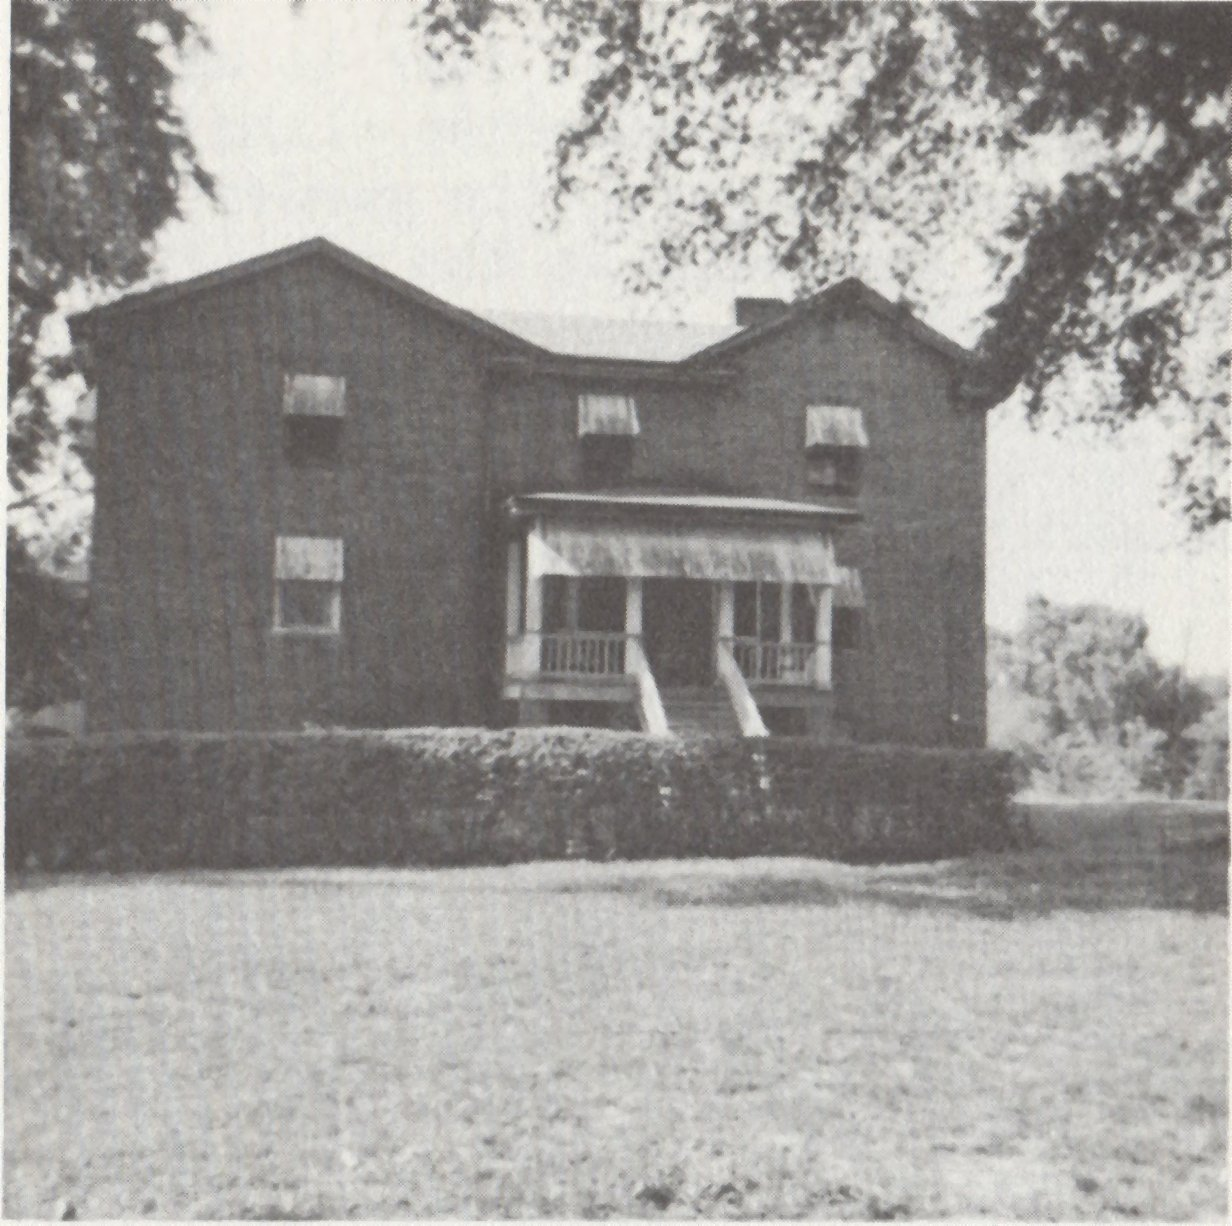
\includegraphics[width=.9\textwidth]{house_photo_1970.jpg}
\end{figure}
 

THE ELMS

 

THE BRUMFIELD PLACE AS IT LOOKS TODAY

 

It was a happy day when the building was complete.  Some of the family thought they ought to select a new name for the farm since it had a new owner and nearly a whole new house.  Several suggestions were made and ``The Elms'' generally agreed upon, but only the romantic young ever used it.  They proudly put the name on the letters written from there, but to most people the farm was simply ``The Brumfield Place''.

 

The house still stands but it is not in good condition.  It is not even in condition to justify the great expense of restoration assuming a fabulously wealthy person could be found with this laudable whim.  However, the house is occupied and is quite comfortable in summer.  Electricity, well water and inside plumbing have been added, and a modern kitchen is set up on the second floor.  In winter a coal burning stove keeps the lived-in rooms warm.  All is fine unless the pipes freeze, but this is a thing very likely to happen.  Except for the yard the areas near the house have grown up in brush.   Most of the out-buldings are gone or abandoned and the farm land is rented.  The house itself is there, a monument to a busy happy time when a large family lived there and loved it.
 
\pagebreak
\poemtitle{The Elms}
\begin{verse}
The old brick house beside the road,\\
\vin Its silent vigil keeping,\\
The rooms and halls deserted now\\
\vin Were once with laughter reeking.

The old home place so dear to us,\\
\vin Those vivid memories cling,\\
The house, the yard, the garden too,\\
\vin The elm trees at the spring.

Dear old home, we love you,\\
\vin Big yard with welcome shade,\\
Broad stairways, too, and spacious halls\\
\vin Where happy children played.

Their voices echo through the halls,\\
\vin Tho really all is still,\\ 
For those of us who loved thee most\\
\vin Are sleeping on the hill.

The rest of us with weary feet,\\
\vin Far from thy threshold roam,\\
Within our hearths this fervent prayer,\\
\vin God keep our dear old home.
\end{verse}

\begin{flushright}
Carrie Brumfield Smith
\end{flushright} 


\section{The Brumfield Place as it Used to Be}

 

The house faces almost due south.  Travelers usually come from the direction of Renan a mile and a half away to the west.  The road from Renan and all the land on both sides of it were part of Henry Brumfield's farm (at one time he owned fourteen hundred acres).  When the road makes a sharp right angle turn around the stripping barn the house is first seen.  Looking beyond the family cemetery down the hill across a wheat field and the little creek the house stands some three hundred yards away.  Its tallest side, the old brick ell, is toward you; its lines are simple and solid rather than beautiful, but this first sight is a heart-lurching thrill to those who loved it.

 

Arriving at the house there is a large area in front of the fenced yard for the house is set well back from the road.  The carriage or buggy house (too small to garage any car but a Tin Lizzie when autos came in) was to the right of this area.  The yard was a big square, fenced across the front with a carefully made picket fence.  Horses of visitors were tied to this fence or to trees in the parking area.  The other three sides of the yard had a fence of post and board style backed up with chicken wire around the flower garden.  Inside the front gate a straight shady walk led to the steps.

 

[Photo of the house with no shutters, origin unknown]
 
\begin{figure}[h]
\centering
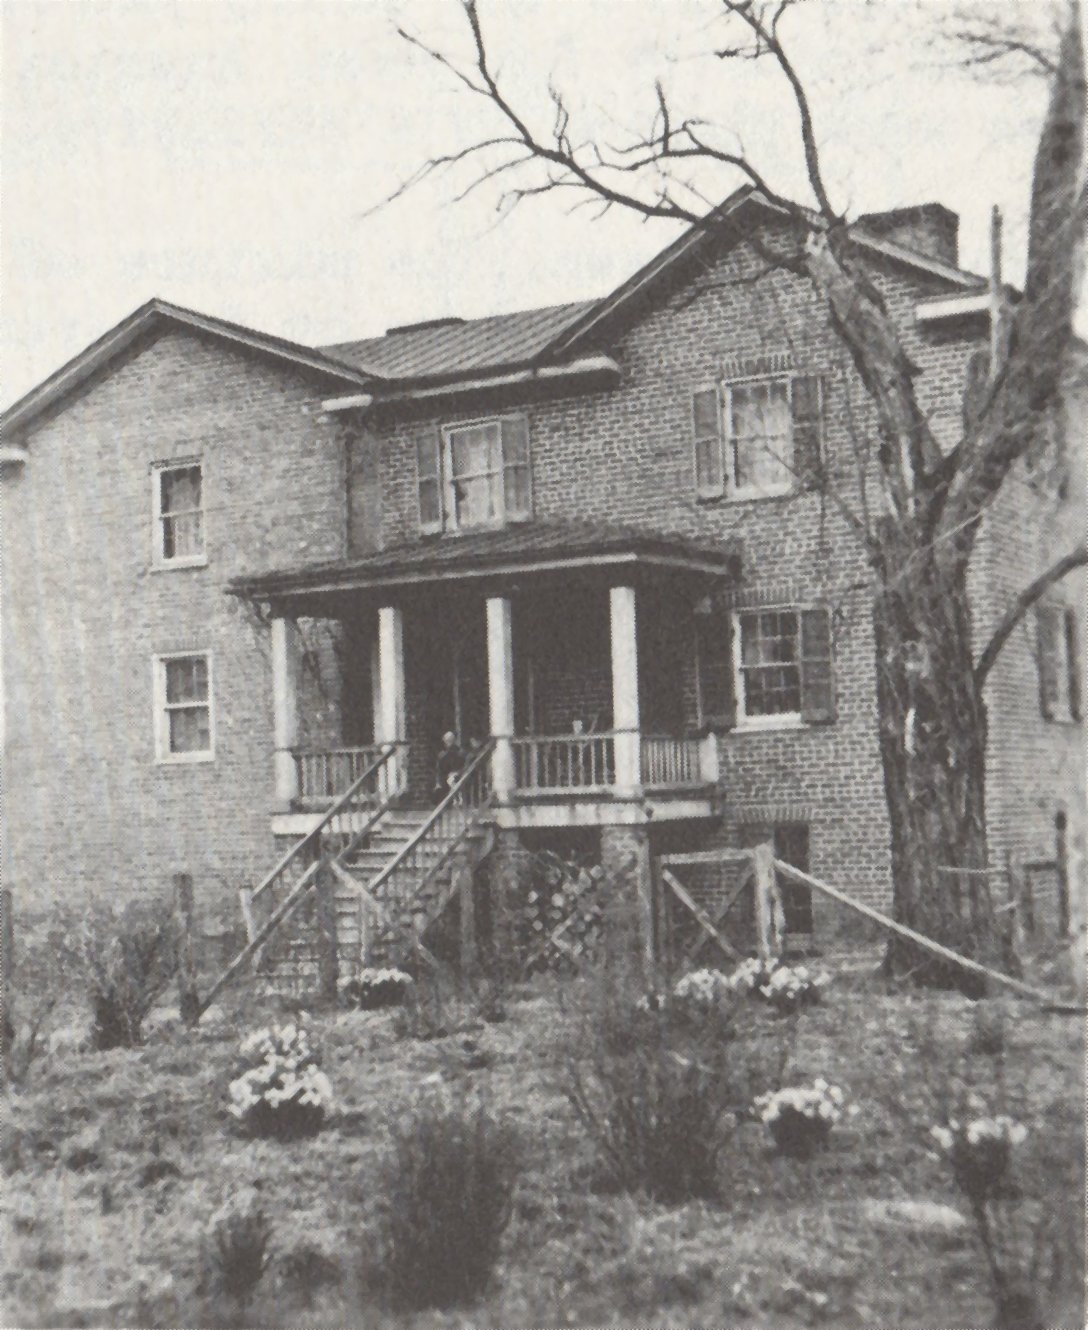
\includegraphics[width=.9\textwidth]{house_photo_1920.jpg}
\end{figure}


The ELMS as it looked about 1920

 

\section{Grandmother's Flower Garden}

 

To the right of the front walk and taking up the whole corner of the front yard was Julia Craddock Brumfield's flower garden.  It had a utilitarian wire fence, hopefully chicken-proof.  The flower beds were laid out in diamonds, circles and squares with sandy walks between them.  The flowers were old-fashioned perennials such as bleeding-heart, lily-of-the-valley, peonies, flages, sweet violets, and the like.  There was a cinnamon vine on the fence with its fascinating little �potatoes�, a snow-ball bush and some roses.  The spaces between the perennials were planted with annuals.

 

This garden was our grandmother's hobby.  No one was required to help her tend it, but she sometimes let a responsible child work there as a special treat.  Good children were allowed to enter the garden and look at the flowers if they were careful to shut the gate, stay on the paths, and not pick anything without permission.


\section{The Yard}

 

The house had no foundation planting.  Once there were large American elm trees in the front yard, but a fifteen-year-old son, proud of hid skill with an axe, cut most of them down and planted trembling aspens.  Two enormous pink mulberry trees grew in the back yard, but their fruit was of interest only to chickens.  These trees were introduced into Virginia as food for silk worms at the suggestion of Thomas Jefferson.  In the 1600's the colony had raised some silk, and he thought it a good industry for young America.  No silk was raised here, the trees were planted as a curiosity.

 

There was never much of a lawn.  The mixture of wild grasses was mown in summer, but was mostly kept down by free-running chickens and other farm animals temporarily pastured there.  Grass was kept neatly chopped from the front walk which was swept daily with a brush broom.  The leaves were raked and burned in the fall.

 

Little triangular shelters or coops for a mother hen and her brood were put here and there about the back yard.  Grandmother loved tending chickens.  She set her hens early and as the eggs hatched she brought the baby chicks into the house where she kept them in a box made cozy with an old piece of flannel cloth and placed near the cook stove.  When all the eggs were hatched the brood was put with the mother hen in one of the coops.  The hen was shut in for a few days to be sure she would take on the responsibility of motherhood.  Pans of water for the chickens had to be kept filled, and they were fed twice a day.

 

If the baby chicks were sick Grandmother doctored them.  There is a parasitic worm which lodges in the throat of baby chicks.  When Grandmother saw the symptoms she would take up the baby chick and gently pry open its beak and remove the worm with a loop of horsehair.

 

The yard had one out-building, the smoke house, located near the back door.  It is (for it is still there) about ten feet square built of brick with a pointed roof.  The only openings are the door and a vent near the peak of the roof to let the smoke escape.  When meat was cured a smoldering fire of hickory wood was kept in the clay pit in the center of the floor.  The meat hanging above it was surrounded with the fragrant smoke for about two weeks.  The result after a period of aging was genuine Virginia ham, an unsurpassed delicacy.

 

[Sketch of smoke house, chicken shelters, beehives, and fencing]
\begin{figure}[h]
\centering
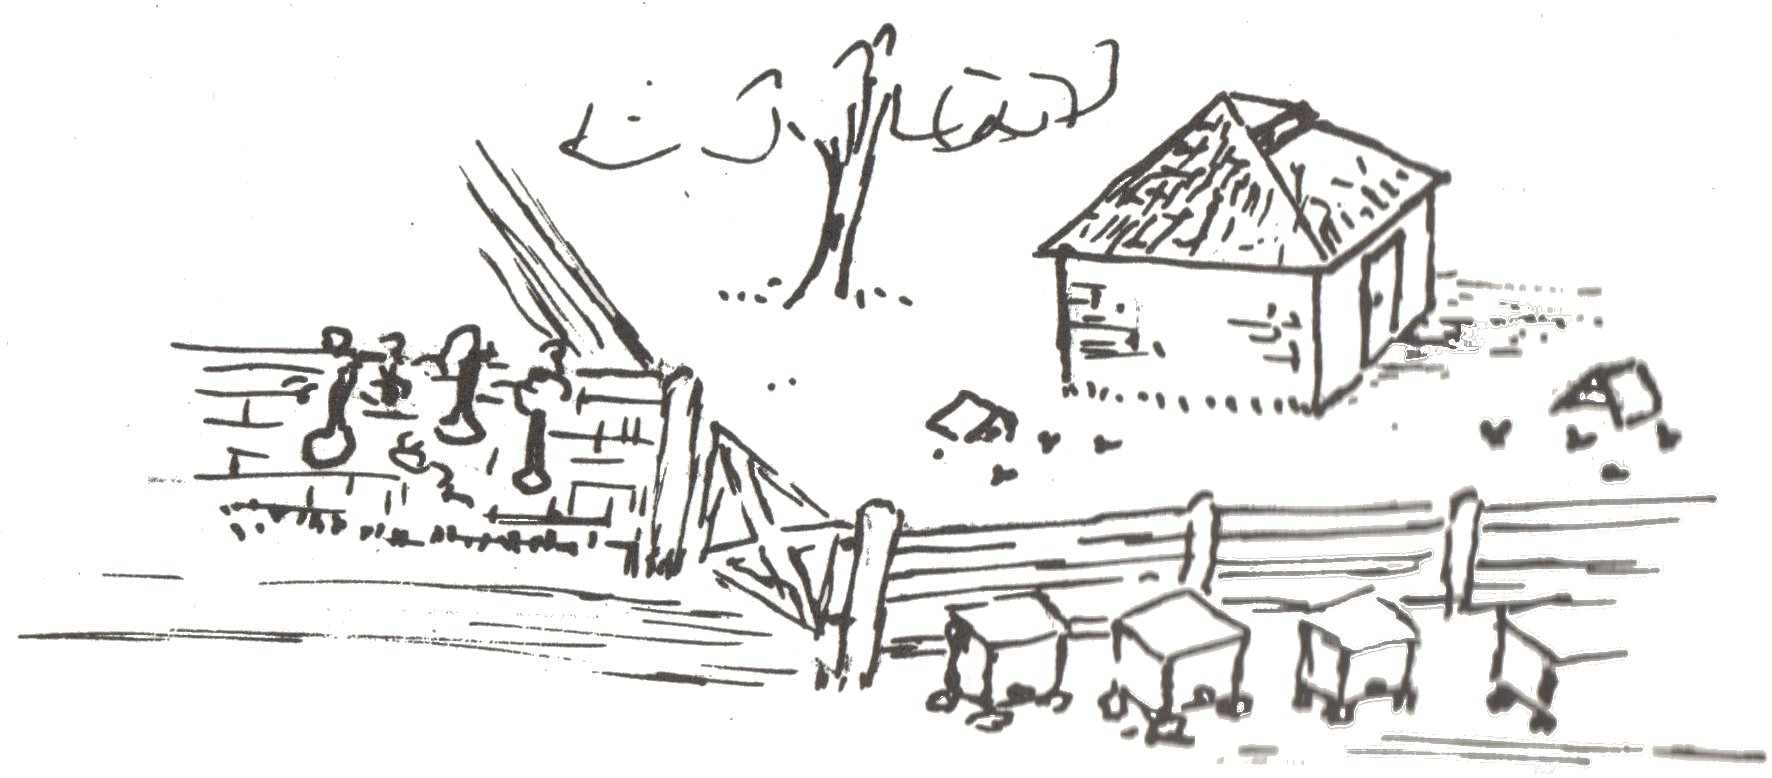
\includegraphics[width=.9\textwidth]{smokehouse.jpg}
\label{}
\end{figure}

 

[Sketch of second floor, labeled �SECOND FLOOR PLAN: ROOM SIZE APPROX�]
\begin{figure}[h]
\centering
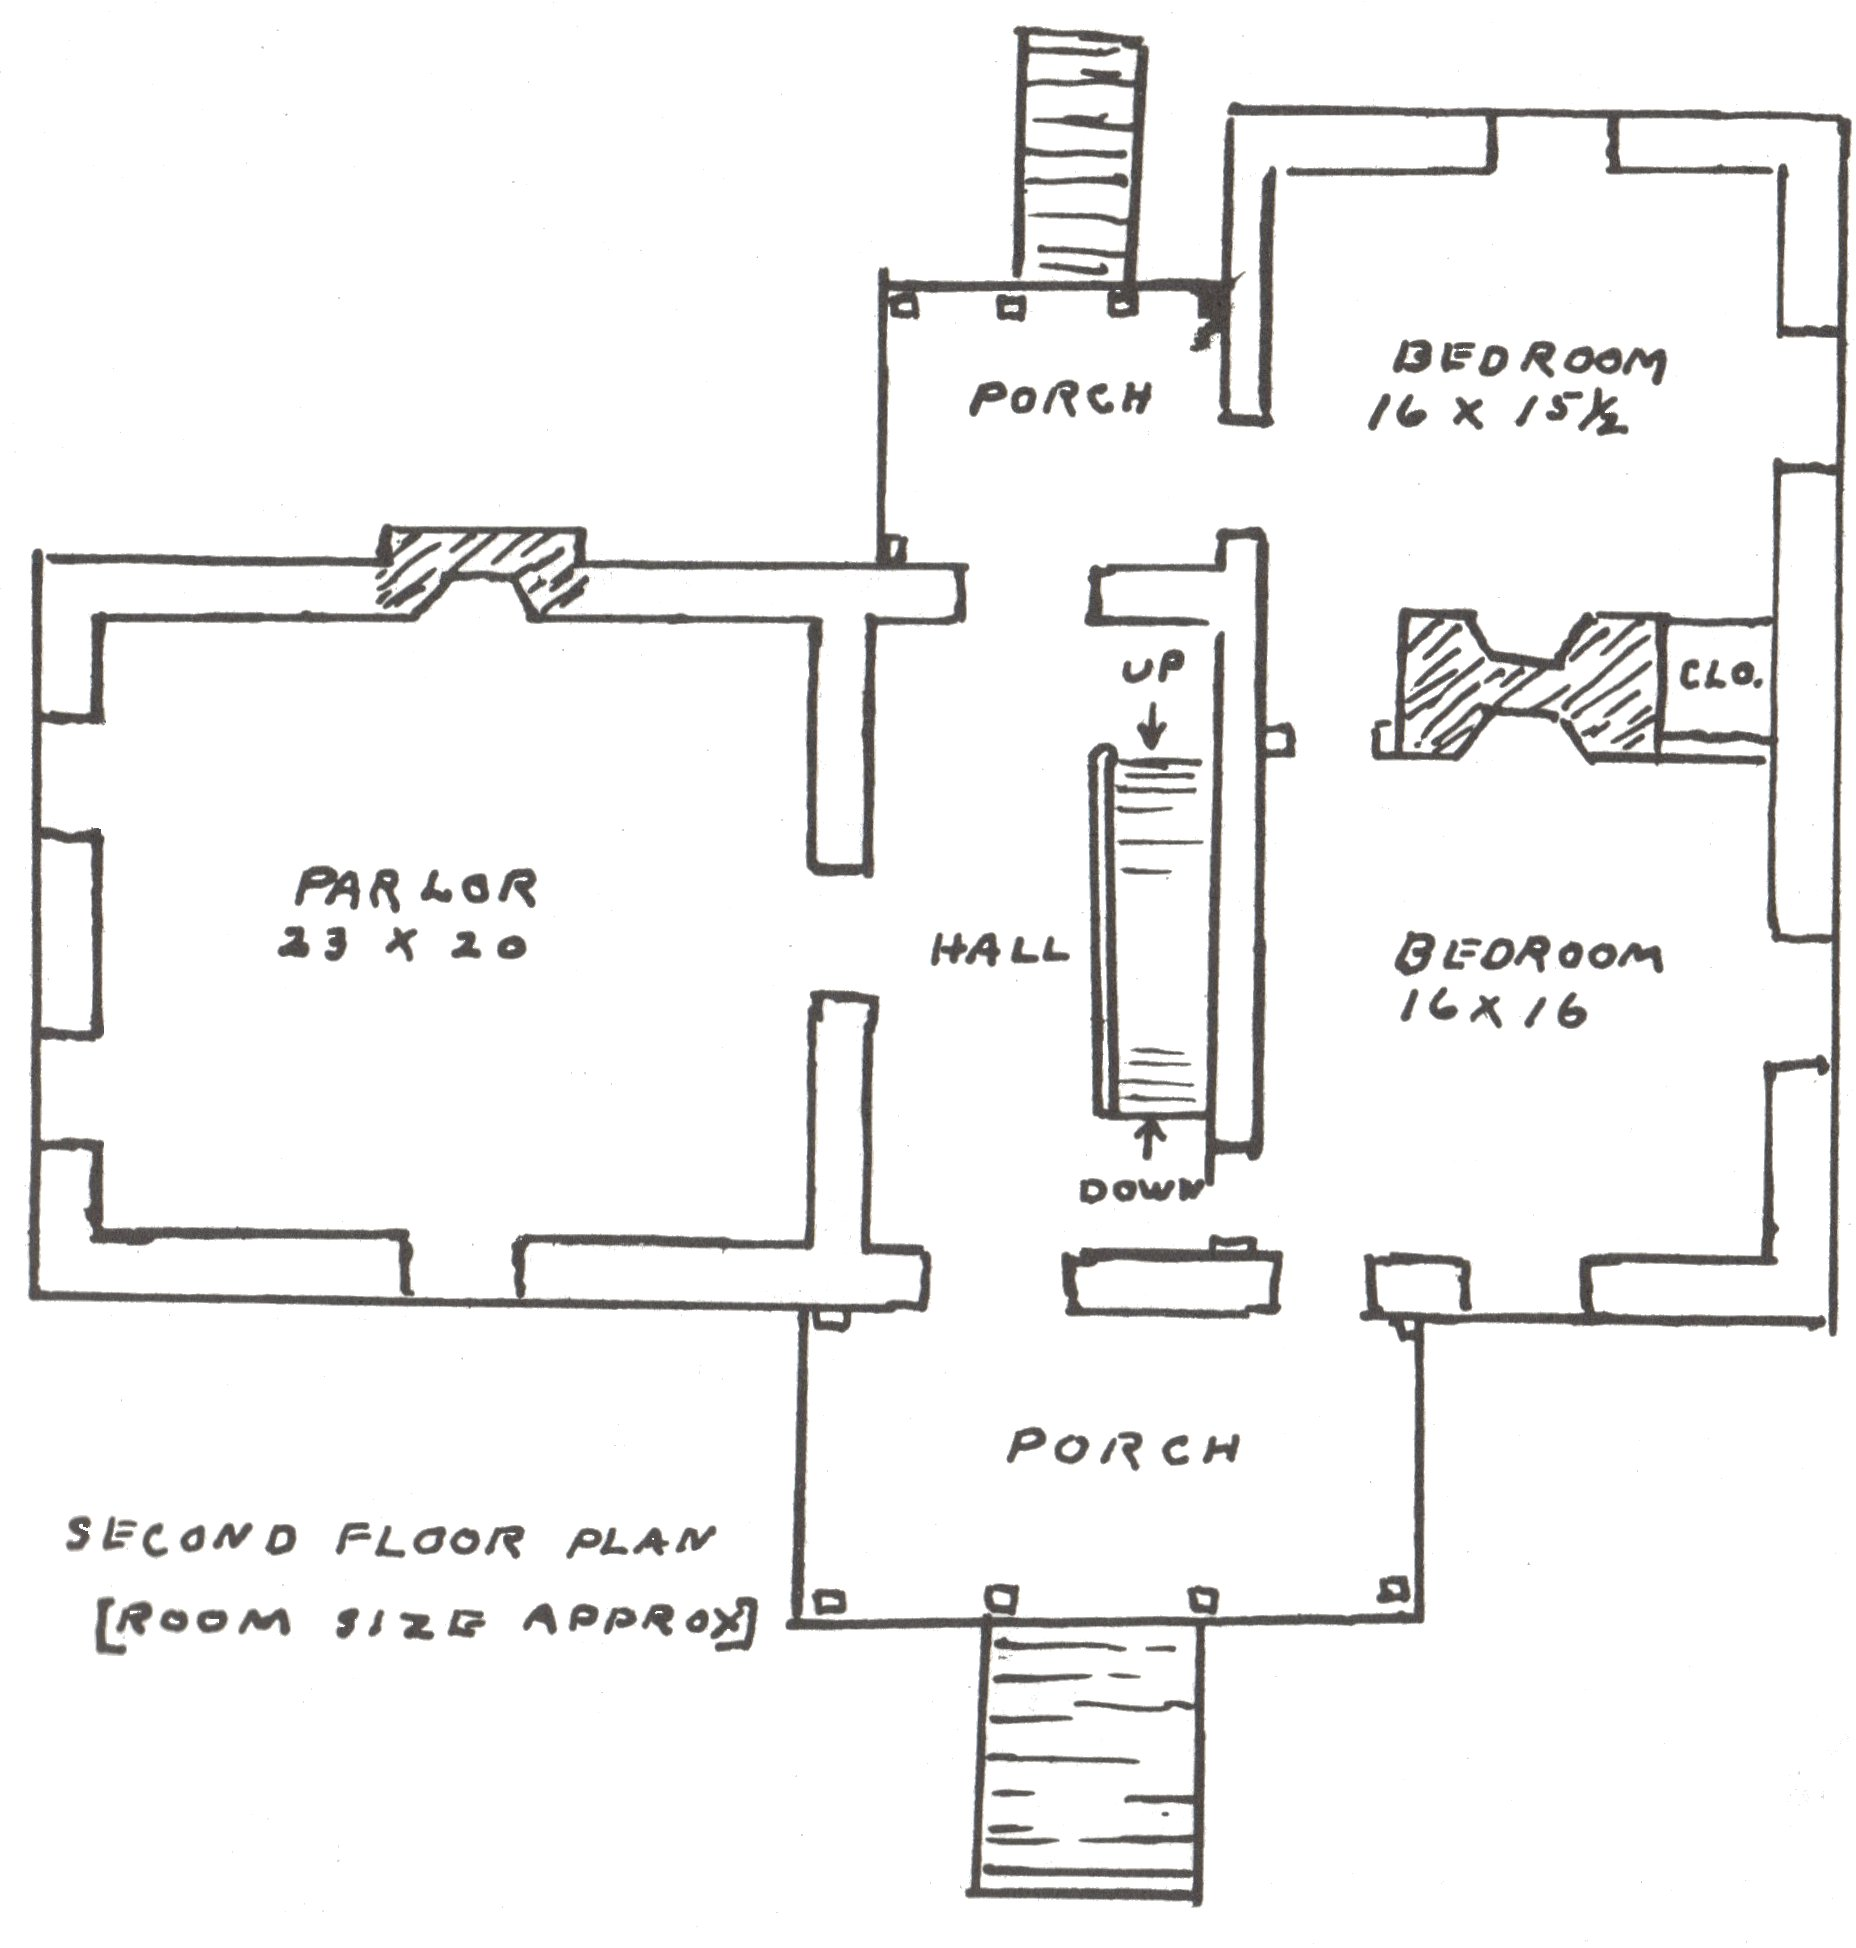
\includegraphics[width=.9\textwidth]{second_floor_diagram.jpg}
\label{Second Floor Plan: Room Size Approx}
\end{figure}

 

\section{The House Inside}

 

It may seem illogical to start the description of a three-storey house with the second floor, but that is where the parlor was.  The front steps led up to a large porch at this level.  The wooden steps are wide, of easy pitch with rails and slender balusters matching those around the porch.  The main front door is paneled and flanked with glass-paned sections.  It opens into a wide hall which originally had a door at the other end opening onto a back porch.  When both doors were opened the hall became a breezeway, a pleasant place to sit in summer.  The only pieces of furniture in the hall were a marble-top pedestal table and a rocking chair.  Hats and wraps were hung on the wall to the left of the door and other chairs were moved in when needed.

 

The stair well is on the right side of the hall.  The stair leading to the third floor rises from back to front, which is a pity since it does not show from the front door.  It is handsome with a nicely turned rail and slender balusters which continue around the stair well on the third floor.  A boxed-in stairway is under this.  Its door is near the front bedroom door and it leads to the ground floor.

 

The parlor is the whole second floor of the old brick ell.  It measures twenty by twenty-three feet, and its proportions are pleasing.  The door is in the center of the east wall and the opposite wall has two windows; the fireplace which is of simple design with a wooden mantle is on the north wall, with one window on the wall opposite it.  There is a painted dado to chair rail height all around.  The windows, like all the others in the house, have wide sills.  The double-hung sashes have no counter-weights to keep them open but on some of the windows are neat notched buttons for this purpose.  Others must be propped open with sticks.  Formerly all the windows had outside shutters which could be closed and latched in stormy weather, or against the broiling sun.

 

The parlor furnishings changed over the years.  Some early pieces were given to daughters when they married; worn-out and out-moded things were replaced and daughters-in-law who came there to live brought some things of their own.  Early descriptions of the parlor mention valence boards at the windows concealing the wooden curtain rods and rings.  They were painted black picked out with a few lines of gold.  There were winter curtains of heavy green and gold figured fabric and summer curtains of lace panels.  A green and gold upholstered sofa stood between the windows opposite the door.  It was made of a light-colored wood of the asymmetrical type or Greek style with the curved back higher on one side than the other.  An oil painting was hanging above it.  This painting was of a rural scene with a cow in the foreground with her face turned to look out of the picture.  These details are given by one of the older granddaughters.  They are fixed in her memory because as a small child she stood on the sofa and poked a pencil through the cow's eyes.  She must have been spanked or scolded or both, and she harbored a feeling of injustice because the holes were already there, made by some unknown miscreant who got away with it.

 

There was another sofa of similar style, but upholstered in red and made of dark wood.  A round center table held the lamp and there were several other tables in the corners, one with a vase of dried pampas grass on it.  Near the door there was a small marble-top chest with a pitcher and glasses for fresh water to offer guests.  Two large rugs which had been woven at a North Carolina mill from wool grown on the farm were used in the parlor.  They were not the thick, heavy kind with burlap backing  but were all wool tightly woven so they would

 

[Sketch of a child poking a pencil through the eyes of a cow in a painting]
\begin{figure}[h]
\centering
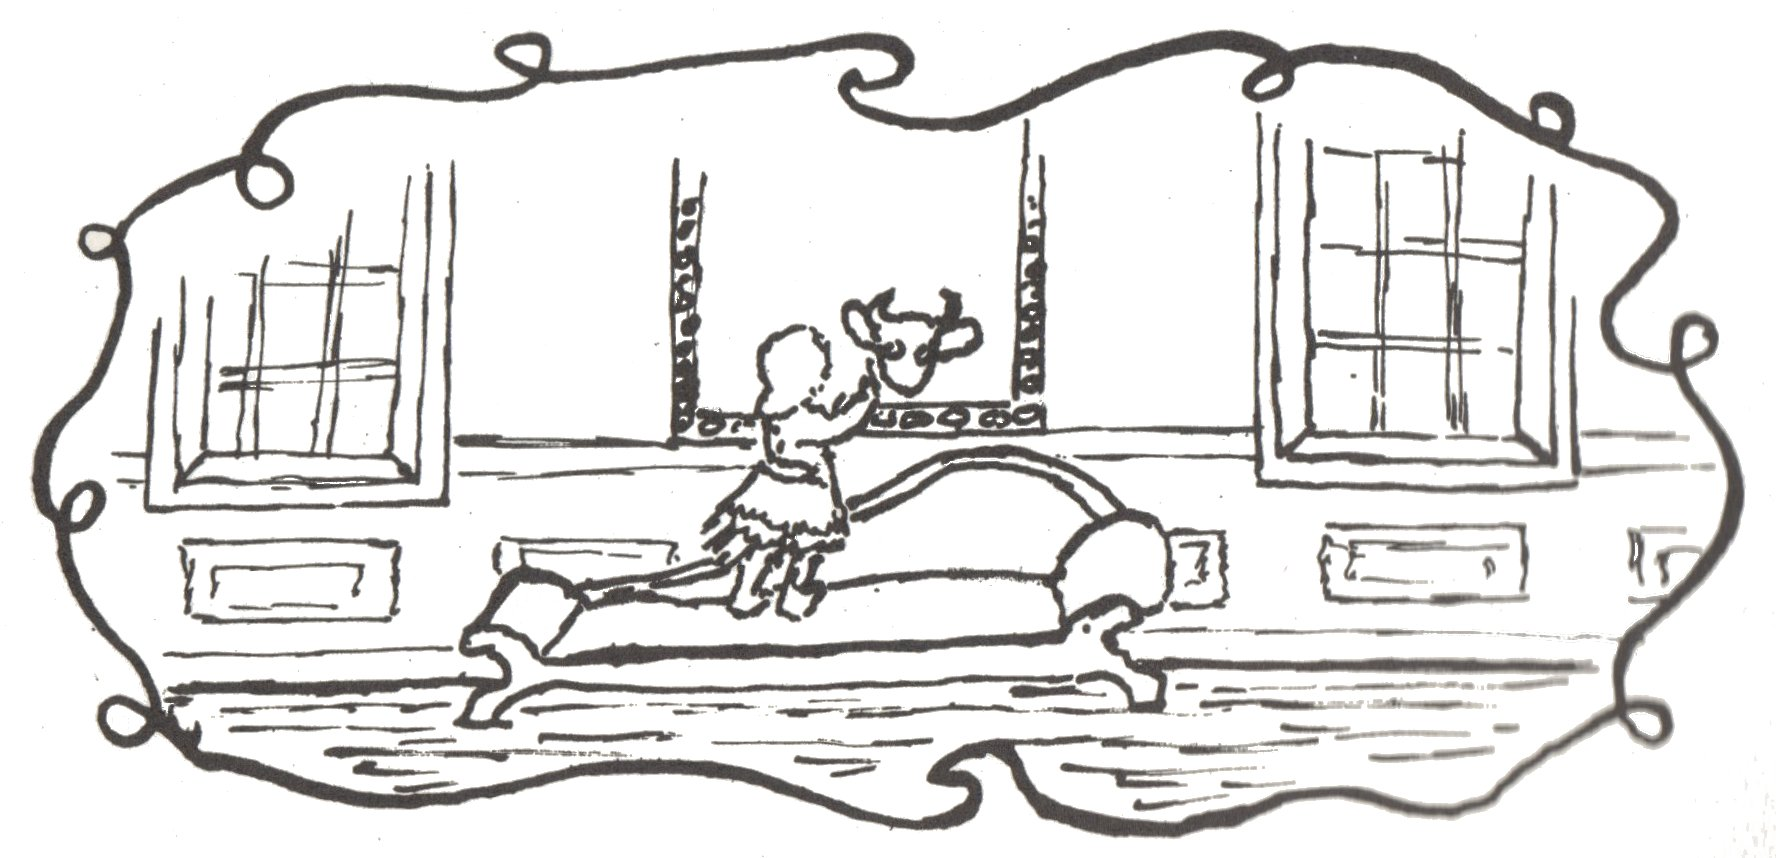
\includegraphics[width=.9\textwidth]{girl_in_parlor_with_cow_painting.jpg}
\label{}
\end{figure}

 

stay smooth on the floor and were reversible.  When these rugs were removed the wide floor boards which were put down with wooden pegs, were left bare except for a small hearth rug and a few others which Grandmother had made herself.  One of these was a flower garden of appliqu�d felt pieces cut from old hats.

 

At a later time a piano, property of a daughter-in-law, stood between the windows where the sofa and painting had been.  There was then a Victorian set of settee and several chairs upholstered in horsehair fabric.  This fabric is woven from the long mane and tail hairs of horses.  It is not dyed but natural �black� horsehair makes a cloth of pleasing gun-metal gray, which wears forever.  This is no wonder for it is very uncomfortable to sit on.  Horsehair is slippery.  The sitter has to struggle to keep from sliding to the floor, and that is not the only hazard; individual hairs work out and stick like needles, especially when the sitter is slipping.  It was amusing to see an uninitiated guest choose one of these seats only to move as soon as politeness allowed to one of the rockers or split-bottom straight chairs.  The latter were made by Henry Brumfield and were most comfortable.

 

Beside the oil painting there were a few other pictures in the parlor.  Most of these were framed prints, but the group photograph of the family which was taken in 1889 was framed and hung there, and the pair of portraits which were painted in Baltimore in 1901 hung on each side of the fireplace for a while.

 

The other two rooms on this floor were bedrooms.  They were connected and only the front one had a door to the hall, but each had a door to a porch.  They were furnished with the usual bedstead and bureau and in addition had wash-stands equipped with bowls and pitchers and other necessary pottery when there is no bathroom.  The back room had a closet built in the jog of the chimney.  Closets were a rare feature in houses at that time, but all three back rooms served by this chimney had closets.

\section{The Third Floor}

 

The big room over the parlor was a dormitory for boys, and it could hold a lot of boys since it was nearly as big as four modern bedrooms.  At one time it had four double beds in it plus the wash-stand, bureau, chairs, and several round-top trunks.  One of the beds was unique.  It was of blond maple with posts about thirty inches high topped with balls as large as croquet balls.  It could sleep two though it was a little shorter and narrower than the standard double bed � provided the two could take its other features.  It had no springs.  Ropes laced across from side-rail to side-rail and head to foot made a coarse netting to hold a corn-shuck mattress.

 

The two bedrooms across the hall are the same size and shape as those below, but are not connected.  Each has a door to the hall, and of course, they had no outside doors.  These rooms had Victorian bedroom sets of heavy dark wood with marble tops on the bureaus and wash-stands.  Sometimes the mantels were draped with lambrequins.

 

[Diagram of the ground floor]
\begin{figure}[h]
\centering
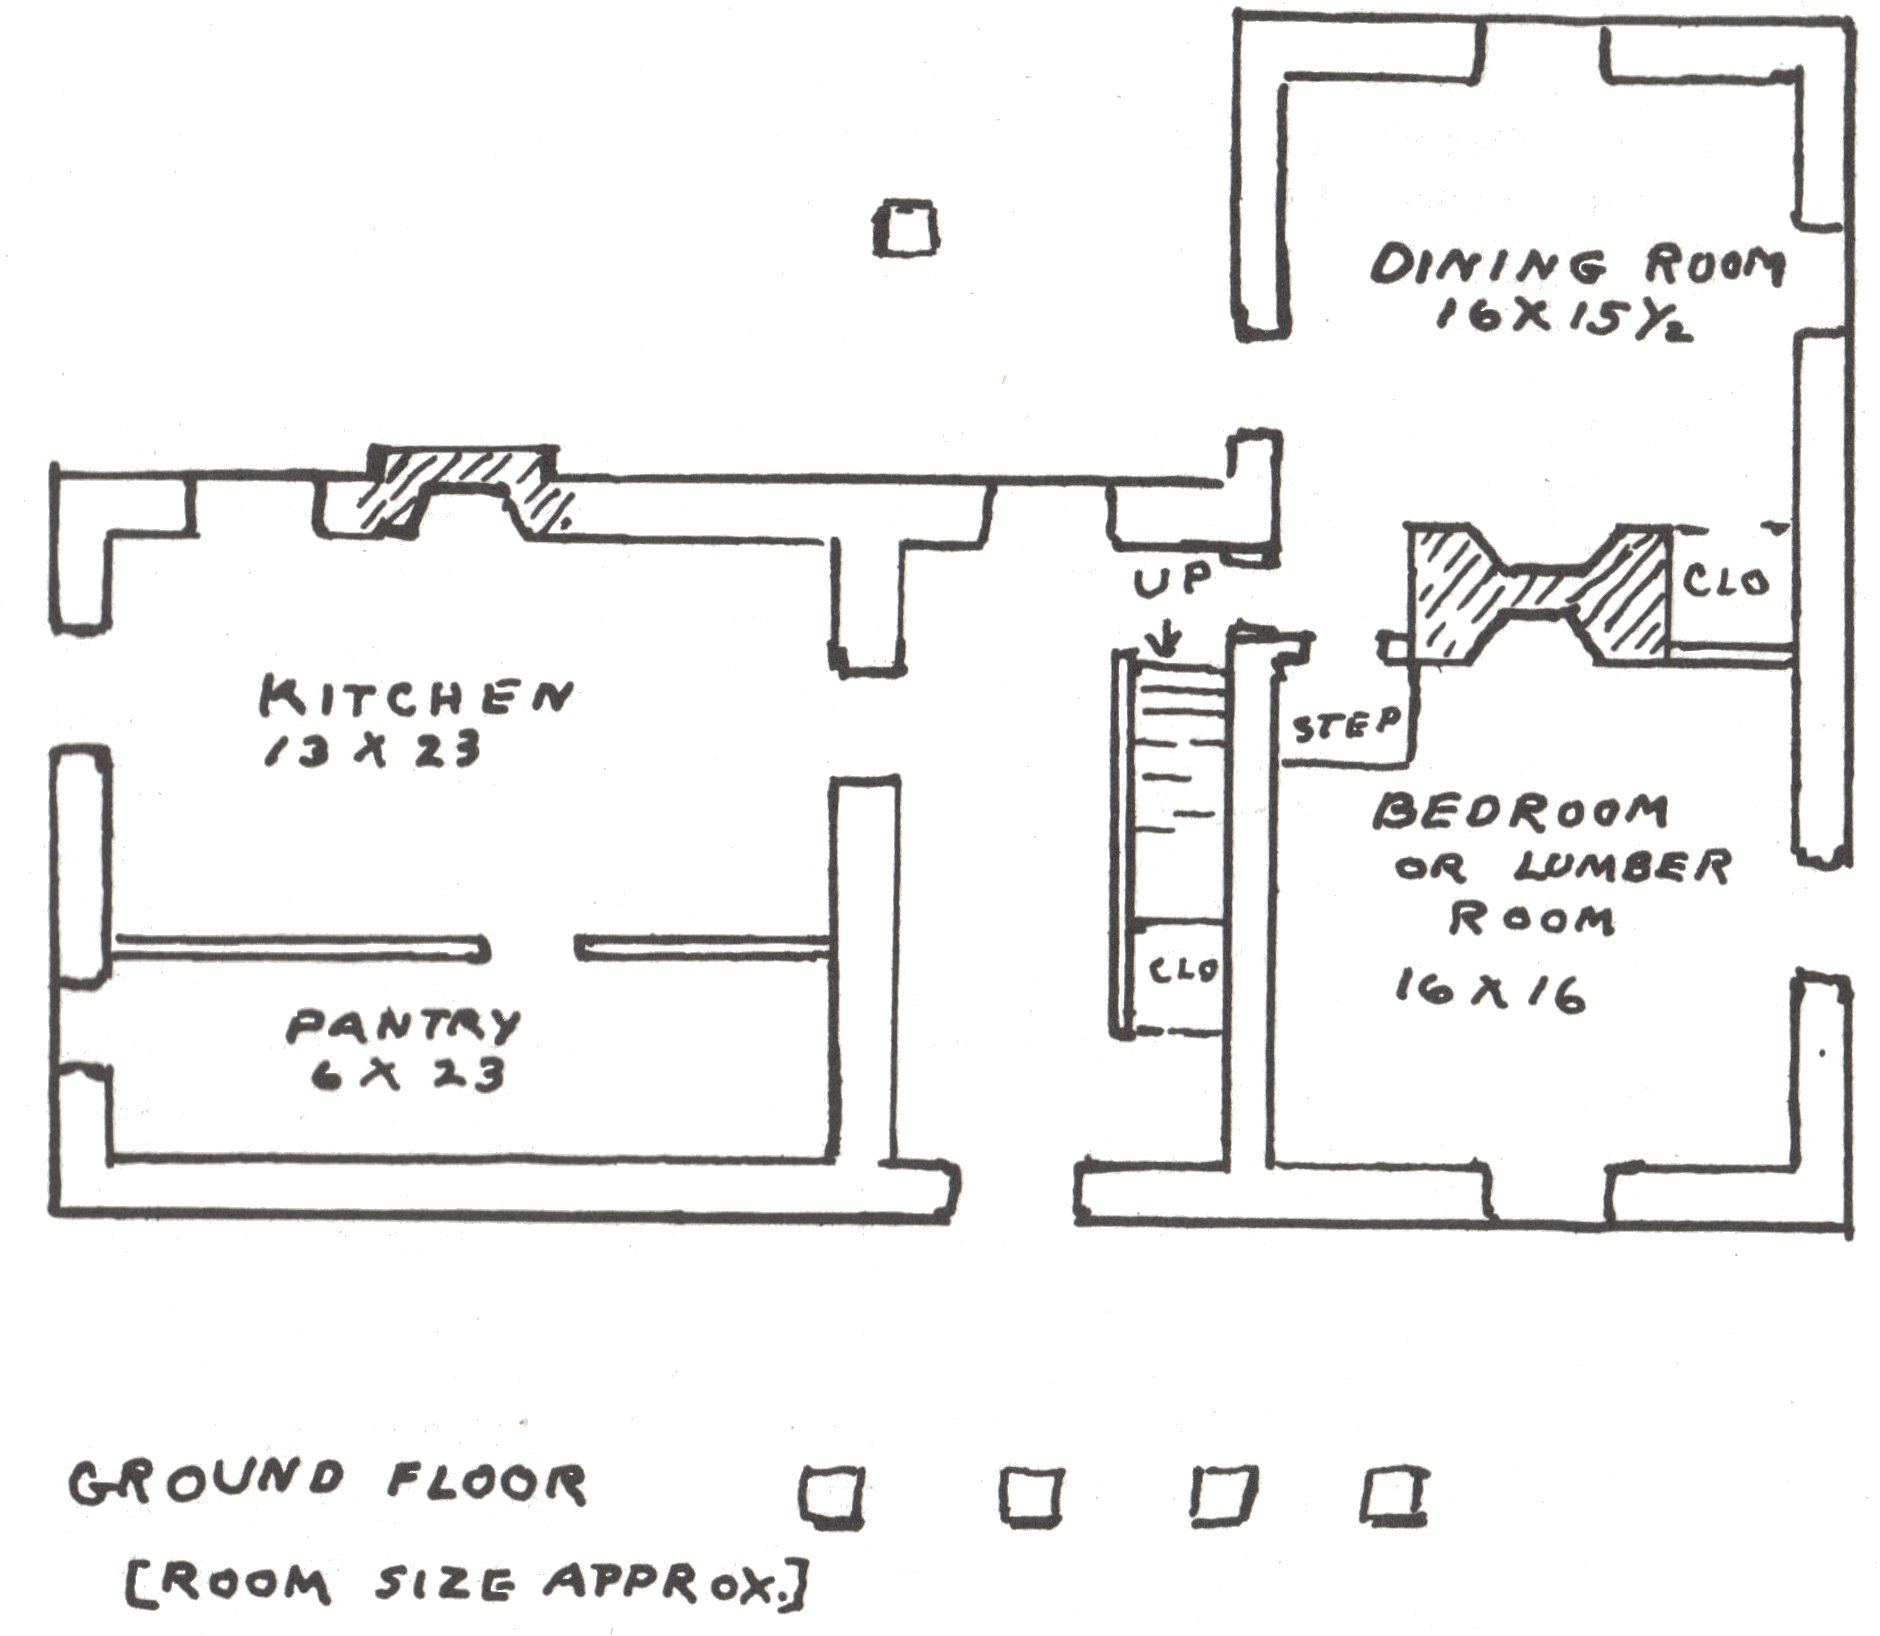
\includegraphics[width=.9\textwidth]{ground_floor_diagram.jpg}
\label{}
\end{figure}

 

\section{The Ground Floor}

 

When the house was completed the ground floor was the center of daily activity since the kitchen and dining room were there.  This floor was built right on the ground, and the new part was actually about eighteen inches below grade.  Termites had never been heard of, therefore no precautions were taken on their account, and the heart pine boards used in the building were known to be highly resistant to dry rot.  Putting wood in contact with the earth was not then known as bad practice, but this was a mistake.  The floors of the dining room and hall had to be replaced several times after the first twenty-five or thirty years, and now the whole ground floor has been long abandoned.

 

\section{The Kitchen and Pantry}

 

The area under the big parlor had been divided into a pantry and kitchen.  The pantry had a single window barred with square wooden bars put there by the first owner.  This was probably done because there was trouble with food thieves during the war, though it may have been done much earlier.  The pantry could hold a year's supply of food and keeping it safe was vital.  Wide shelves behind the door held sweet and Irish potatoes carefully placed not touching each other to prevent rot.  Shelves along the other walls held the crocks of pickles, brandied fruits and honey, as well as hand-woven baskets of dried peas, lima beans and fruits.  There was a sack of green coffee beans.  Coffee was one of the few foods that had to be bought.  It came in twenty-five pound sacks of the green beans.  These were roasted in the oven, a few pounds at a time spread out in a biscuit pan, and the roasted beans were freshly ground just before use.  The aroma of roasting coffee is delectable and the drink made in this way was excellent.

 

Eggs for the table were kept in a large squat gourd.  It had an access hole in the side and the eggs rested on a bed of cotton.  Barrels of sugar, flour, meal and apples stood on the floor along with the big demijohns of vinegar protected by wicker covers.  There were many more wonders not now recalled, for after all this fascinating place was ``off limits'' to children.

 

The Graves once had an outside kitchen, which was usual in early days.  The noise and clutter of preparing meals was kept out of earshot, also there was less danger to the house in case of fire, always likely to start in a kitchen. When the Brumfields first moved there the old kitchen still stood but had not been used for a long time.  It was torn down and a servant's house built on the spot.  The inside kitchen fireplace was equipped for cooking but soon a cook-stove was installed.  It stood beside the hearth with its enormous wood-box in the corner near the hall door.

 

The other corner at this end of the room was taken by a corner cupboard which held all the small supplies and utensils.  This piece had been left by the Graves, and nobody considered it handsome.  When its joints had loosened and its boards warped so that it was no longer useful, it was thrown out.  Luckily a grandson saved the scraps and restored it to beautiful condition.  It is now a prized antique.

 

A big table between the corner cabinet and the pantry door was the mixing center.  Grandmother's large wooden tray for mixing bread which she used for over fifty years, was always on this table, covered with a cloth when not in use.  Fresh biscuits were made for breakfast and mid-day dinner, but warmed-up ones might do for supper.  The lamp was on this table and usually lighted, for breakfast was served at daylight and supper after dark and at best the kitchen was rather dark since it had only one window.  It is not surprising that electric lights were the most wanted improvement, even ahead of piped-in water.  A Delco system was put in when first available, but was soon abandoned because of its inefficiency.

 

At the other end of the room under the window stood the bench for water buckets and the basins for washing hands.  Just outside the back door was a trough for carrying away waste water. It was a great convenience to empty this water from the door-step and not to have to carry it across the yard.  Dish water was never put in this trough.  It along with table scraps went into the two large slop buckets which stood on the hearth, and this mixture was fed to the pigs.

 

There was still plenty of room for chairs for such sit-down jobs as churning, coffee grinding and preparing fruits and vegetables.  Henry Brumfield often joined his wife and daughters at this work, especially in preparing fruits for drying.  He also had sit-down jobs of his own which he liked to do in the kitchen or before the dining-room fire in winter.  He wove the split-oak chair seats and baskets, or polished the new handles he made for his hand tools, or did a job of cobbling.  At one time he had wooden lasts in all sizes, but he replaced these with iron ones.  With these he was able to resole any of the family shoes from scratch, tanning the hides from his own beef.  One of his boys said he made these shoes without a right and left.  The two shoes of a pair were just alike and the wearer was supposed to reverse them every day to equalize the wear.  It sounds miserably uncomfortable, but worn over the well-knitted wool or cotton string socks which Julia and her girls made it might have been all right. (Note: the writer is told that such pairs of shoes are still made for certain sportsmen, who think them great!)

 

The kitchen smelled wonderful.  Besides the delectable smell of roasting coffee there was frying ham, baking bread, pickling peaches and many others.  To a child the very best smell of all was the spicy aroma of baking ginger0bread.  This is our Grandmother's recipe:

 

GINGERBREAD OR GINGER COOKIES

 
\begin{tabular}{ll}
1 cup shortening&
1/2 cup boiling water with -- \\
1 cup sugar&
1 tablespoon soda dissolved in it \\
1 cup molasses&
1 tablespoon ground ginger\\
1 egg&
1 teaspoon salt\\
\end{tabular}


 

Mix the above ingredients in a big bowl and add flour to make a dough.  For gingerbread the dough should be just stiff enough to press out with the hand to a thickness of about a half-inch; for cookies the dough should be stiff to roll out and cut in rounds or oher shapes.

 

Like all old recipes this one calls for judgment on the part of the cook, but with practice it is possible to turn out a fine treat.  A modern cook may prefer to make the dough right for a cookie press.

 

[Diagram of the kitchen]
\begin{figure}[h]
\centering
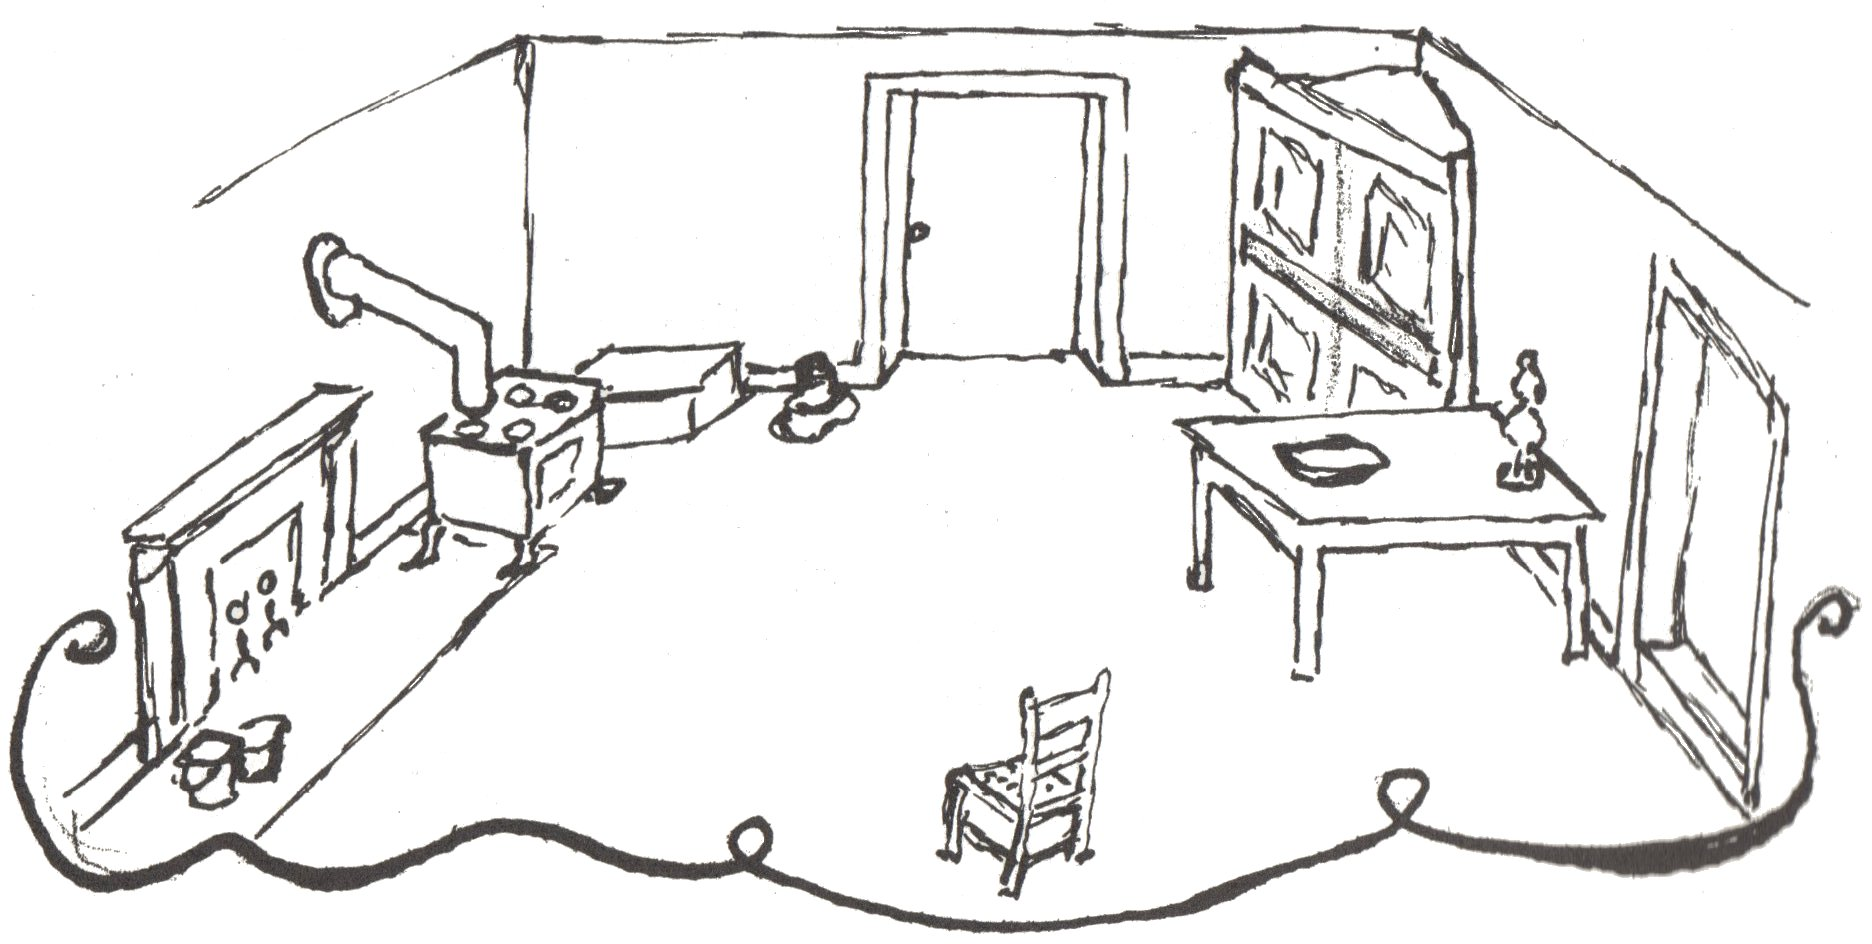
\includegraphics[width=.9\textwidth]{kitchen.jpg}
\label{}
\end{figure}

 

 

\section{The Dining Room}

 

The back room on the ground floor across the hall from the kitchen was the dining room.  Its door was right at the foot of the steps.  This was convenient for family and guests coming from the parlor and other upstairs rooms, and perhaps explains the reverse direction of the stairways.  A door to the outside opened to the area under the back porch.  In summer this was convenient because milk, cream and butter could be brought from the spring house direct to the table without going through the busy kitchen.

 

The dining table was a long oval.  It was made of walnut and was of good design and workmanship but over the years the varnish had softened and the finish was marred by stuck-on bits of lint and paper.  However, the table was never seen because it was always covered with a damask cloth with a drop of ten or twelve inches, put on over a heavy silence cloth.  White cloths were used most of the time but once there were two colored ones used on week days.  These were of red and blue checked damask.  When the ground floor was abandoned the table was left there, abandoned also, until a grand-daughter rescued it and had it restored to its original beauty.  Without its three wide leaves it is round.  There are four turned corner legs and a fifth one in the middle.  The wood is a warm honey color.

 

There were two cupboards, Grandmother's red cupboard and her brown one.  The upper part of the red one was of perforated tin and it was tightly put together and could be kept insect and mouse-proof.  This one was used to keep foods, but the brown one with its many wide cracks could be used only for dishes and when the dining room was no longer used it fell in ruins.  The red cupboard, however, was reclaimed by another grand-daughter and is in use in her recreation room.  Little space was needed to store dishes in any case, for the rule was to set the table for the next meal as soon as the dishes were washed.  The set table was covered with a large white cloth between meals.

 

Grandmother's dishes were mixed remnants from many sets for with so many children breakage was high.  The Haviland tea-set bought to honor the first wedding in the family was of white china decorated with gold bands.  It had acorn-shaped knobs on the tops of the teapot and sugar bowl.  The only piece now intact is the big teapot, which has passed from a grand-daughter Julia to a great-grand-daughter Julia on her marriage in 1969.

 

The wide window-sills served as side tables.  At Christmas time a stone crock of boiled custard was served from there.  It might be flavored with a little brandy.  With it went iced layer cake or dark fruit cake and homemade pickles � fine for party refreshments or bedtime snacks.

 

Canned fruits, vegetables, jams and jellies were stored in the built-in closet which had wide shelves and could hold many jars.  Henry Brumfield kept his shoe making equipment on the floor under the bottom shelf and worked at cobbling before the dining room fire.  Sometimes Julia made coffee and warmed bread for supper at this fire, for she never forgot her skill at fireplace cooking.

 

\section{The Ground Floor Bedroom and Hall}

 

The other ground floor room was at first a bedroom.  It was entered from the dining room and its floor was one step up from that floor.  It also had a door direct to the outside, and this easy egress made it first choice for some of the boys when the family was large and all rooms needed.  This room was Grandfather's bedroom when he was sick and paralyzed, for it was near the kitchen and dining room and when he was able to be up he could take the one step and move about on this floor when he could not manage a flight of stairs.

 

Later this room was given over to storage and Grandmother called it her ``lumber'' or ``plunder'' room.  Fascinating things could be found there.  There was a spinning wheel, a hoop skirt and bustle frame, a lot of old clothes to dress up in and rag bags to explore.  There were back numbers of magazines, some many years old.  These were a special pleasure to a child who liked to read, for the family had very few books.  The Bible, a history book or two, school text books and the few politely fought-over novels which had been left there by visitors were all there were.  The days of a farmer were so filled with interesting things that had to be done there was little daylight time to read for pleasure.  When night came such active people were ready for early bed.  Henry Brumfield subscribed to newspapers and farm journals and he and Julia read them.  Sometimes Henry read from his Bible or the newspapers to his wife and children while they were busy with hand work.  Julia thought reading fiction a silly waste of time. Even when she was old and had time to waste and amused herself with a story or novel she scolded herself too for wasting time on something that was not true.

 

The ground floor hall had an outside door opening under the front porch.  All told, there were eight ways to get in and out of the house. This was a good thing.  The many doors reduced traffic jams and helped to keep the house well ventilated and delayed the inevitable decay.  Country living requires much coming and going.  Firewood, water and foods from the garden, orchard and springhouse have to be brought in.  Ashes, slops, and other wastes have to be carried out.  There are outside chores to do several times a day like milking and feeding the animals.  Many ways in and out are a convenience.

 

[Sketch of coffin rocker in the hall]
\begin{figure}[h]
\centering
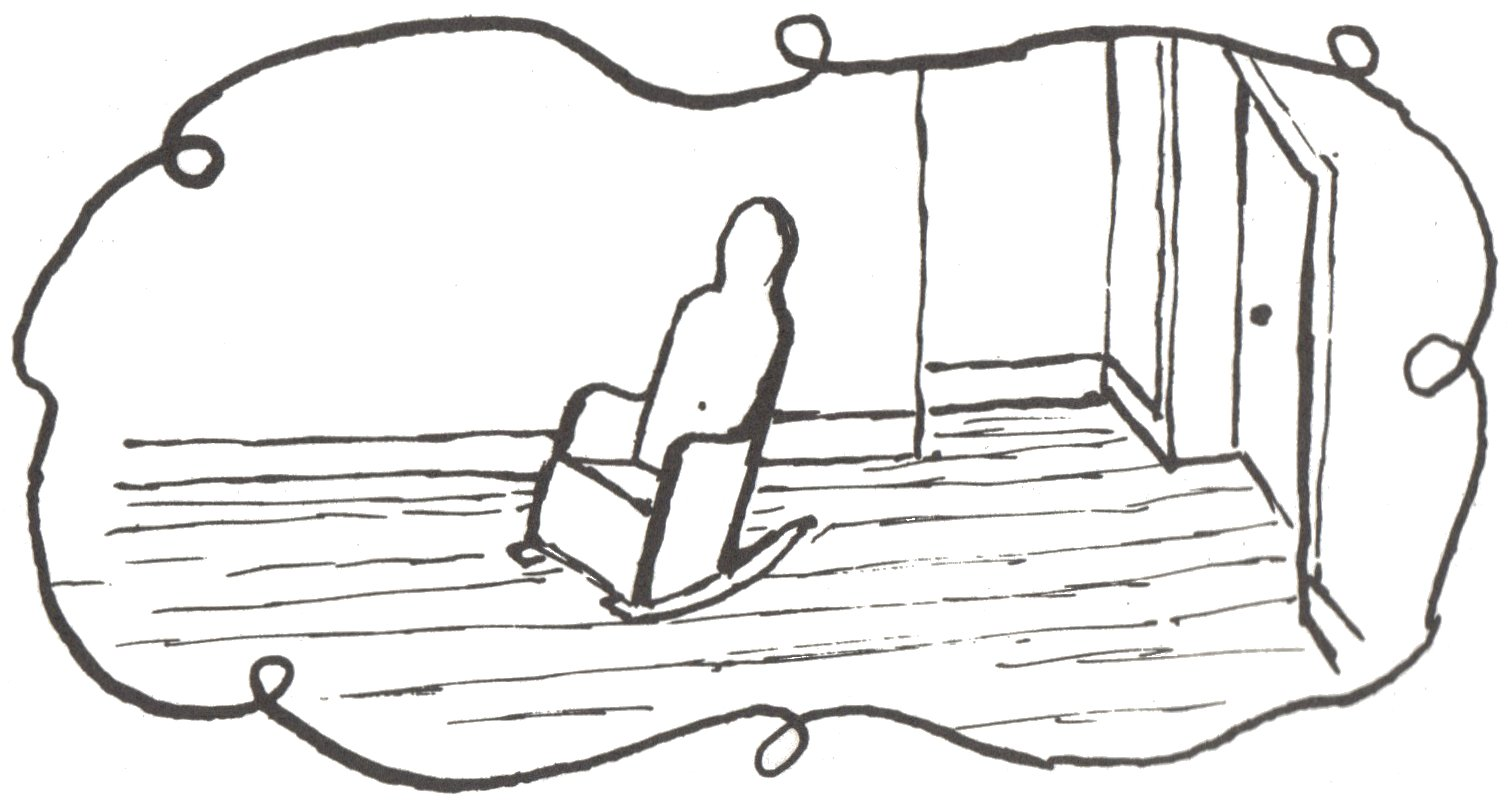
\includegraphics[width=.9\textwidth]{coffin_chair.jpg}
\label{}
\end{figure}

 

There was a unique piece of furniture in the ground floor hall.  It was a rocking chair which looked like a big, black box.  It was homemade of wide boards, so wide each main piece was cut from one board.  The back was higher than an adult sitter's head and was shaped to resemble a head and shoulders.  The arms had a comfortable curve at the top but they were only the thickness of the side boards and therefore hardly wide enough for their purpose.  These sides fitted onto rockers at the bottom.  The seat was a little wider at the front than at the back and was a snug fit for the average sitter.  The whole thing was stained black, fearfully suggesting a coffin to an imaginative child.  Grandmother found it comfortable, however, and she often rocked babies in it and chose it for cat-naps.

 
\begin{figure}[h]
\centering
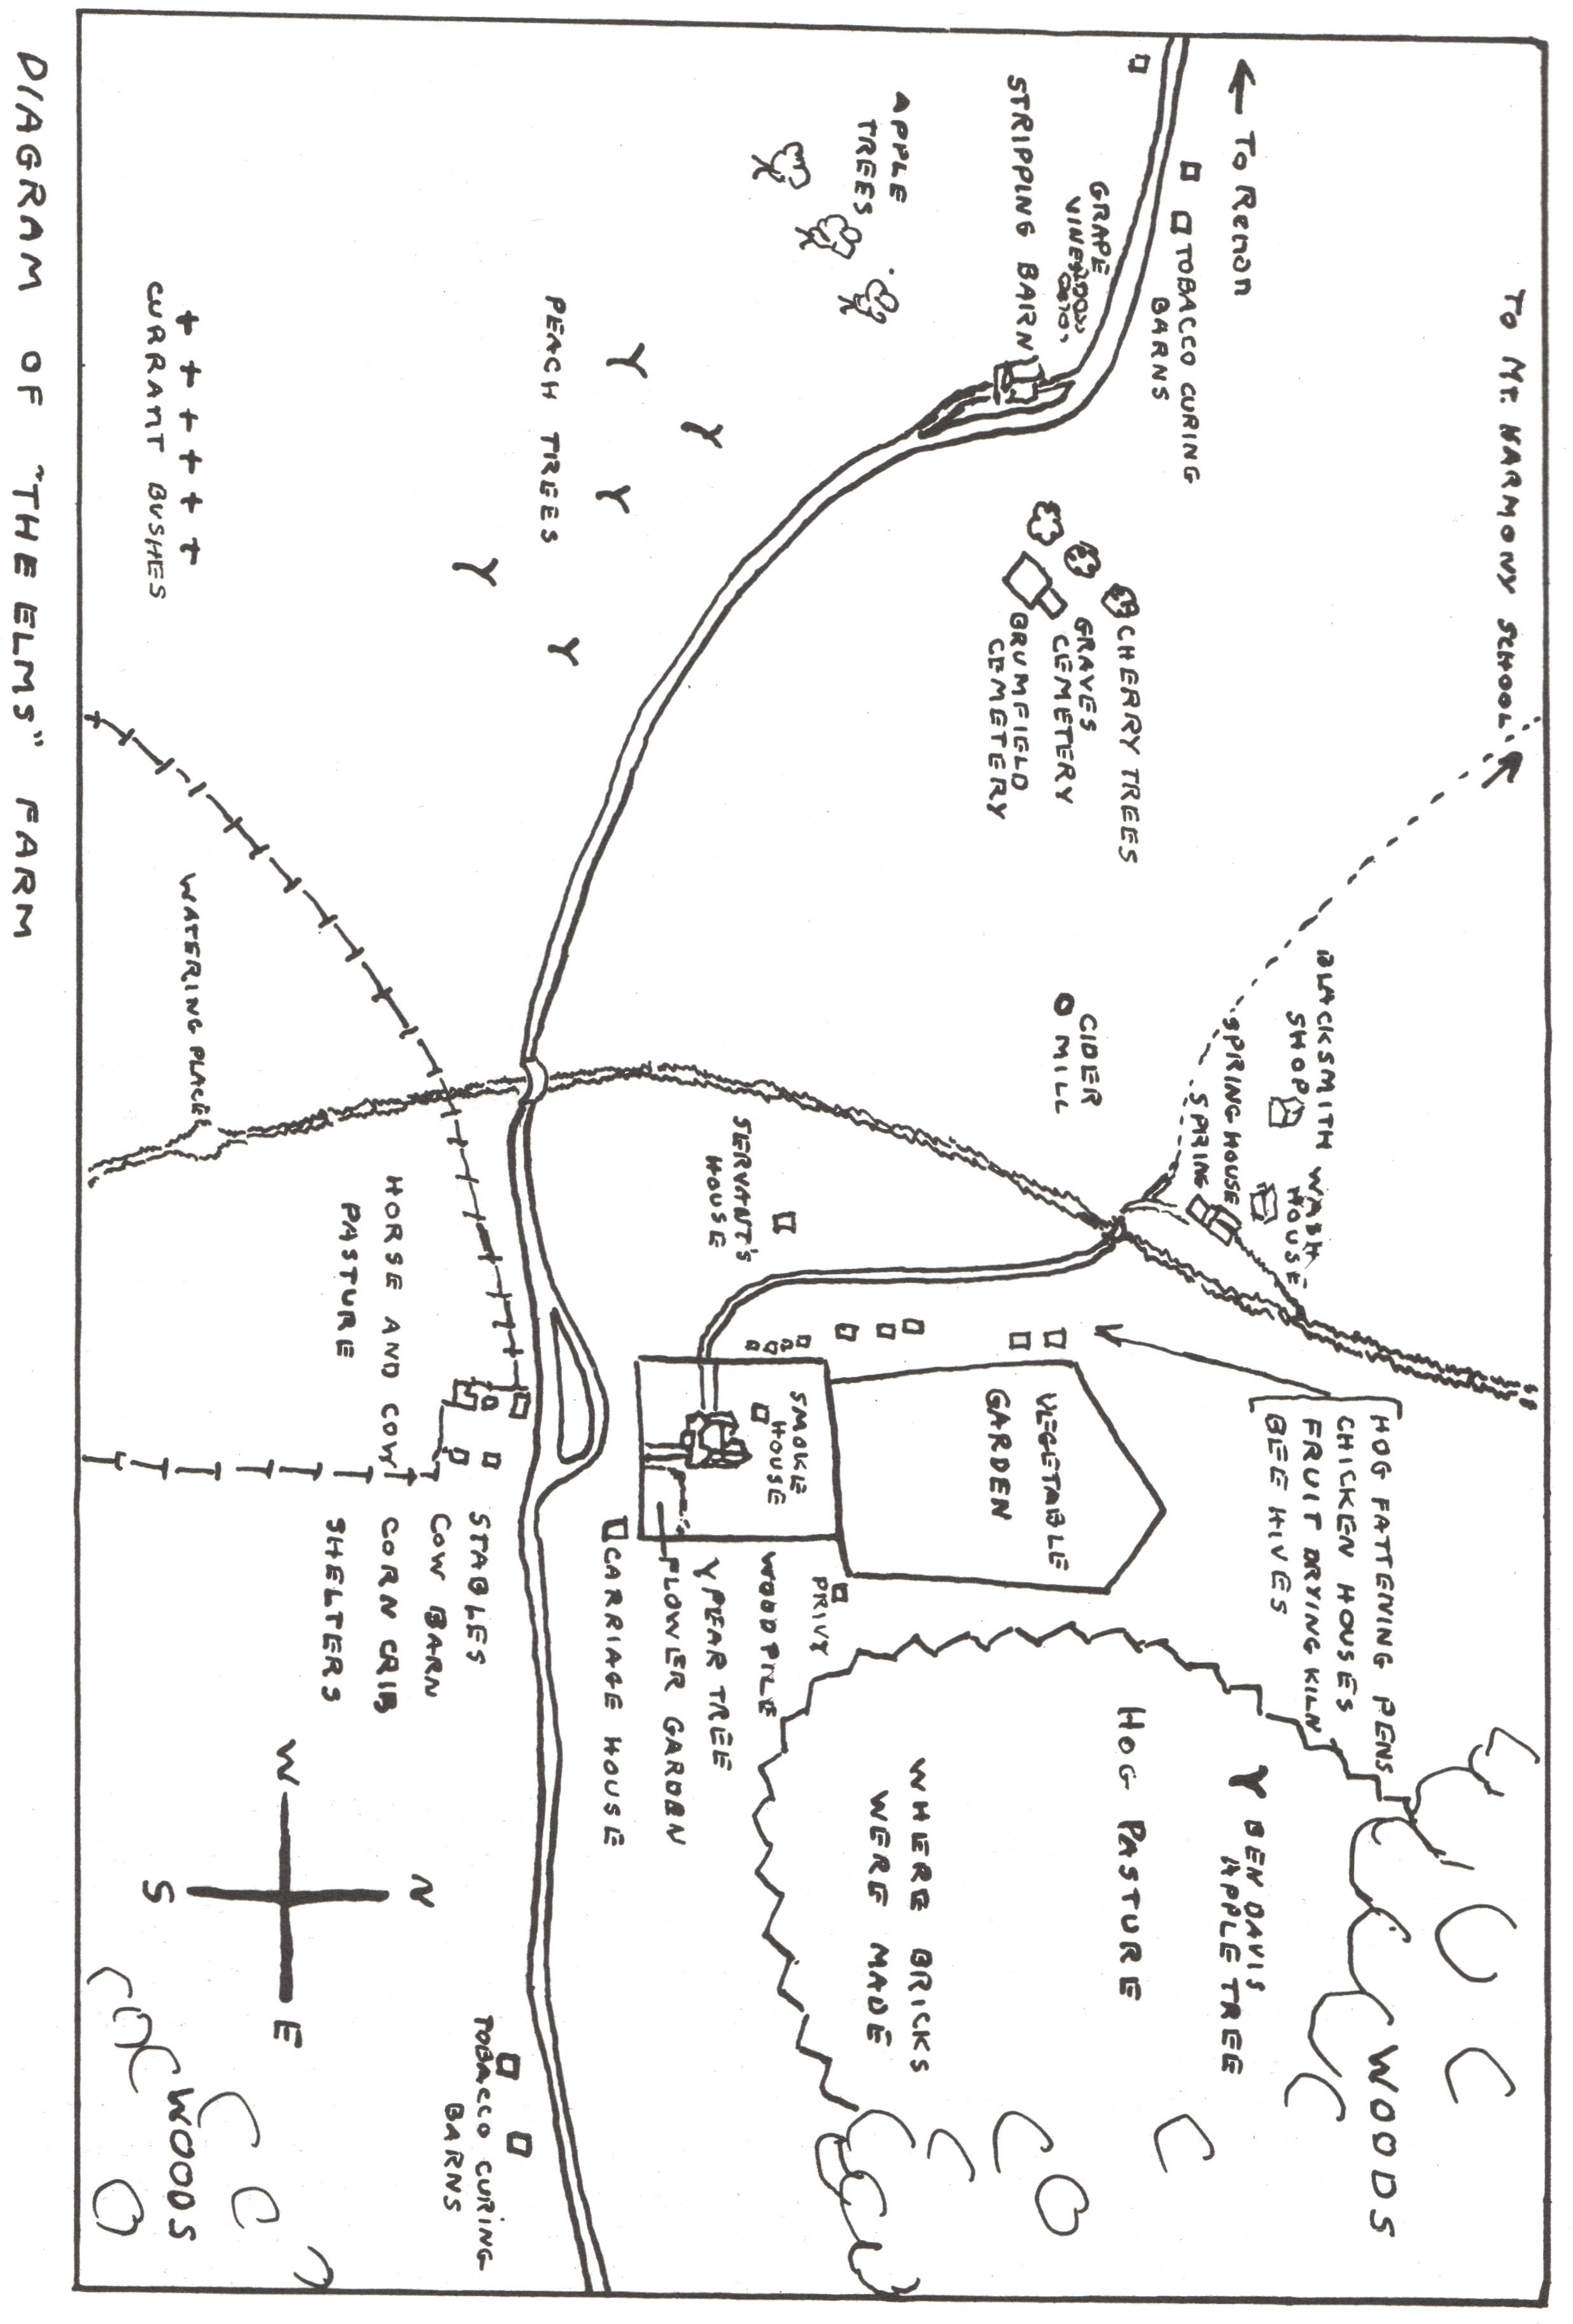
\includegraphics[width=.9\textwidth]{diagram_of_farm_rot_90.jpg}
\label{}
\end{figure}

[Map labeled DIAGRAM OF ``THE ELMS'' FARM]

 

\section{The Environs}

 

Out-buildings are important to farm living and this farm was well supplied.  The privy or garden house or ``necessary'' as the Williamsburg restorers so delicately call it, was located outside the backyard fence and a little beyond the corner of the garden fence.  It was a well-built structure with the door modestly screened with lattice work.  There were three adult holes and a low small-sized one for children.  Visiting the garden house was a sort of social affair, for several ladies might go there together and sit and talk for a while.  This house was built over a ``draw'' where a hard rain could flush it.  This was before germs were recognized as dangerous, or even believed in.  Later a sanitary privy, built to Virginia State Health Department specifications replaced it.

 

\section{The Woodpile}

 

The enormous woodpile which supplied the kitchen stove and nine fireplaces was outside the yard on the east.  Trees were felled in the woods in fall and winter and brought there where the logs and branches were cut into proper lengths for use.  For kindling there was light wood and chips.  Light wood is the inner part of pine tree stumps, so full of rosin it burns with a quick hot flame at the touch of a match.  A few splinters of this under dry chips made fire-building easy, except after long rainy spells when there was no dry wood.

 

Jerusalem artichokes had at one time been planted near the woodpile.  They ran wild and grew there for years, and some children liked to dig and eat the roots.  Also nearby a Seckel pear tree and a white grape vine bore fruit that rewarded a child whose duty it was to keep the kitchen wood box filled.

 

\section{The Vegetable Garden}

 

This garden, located just back of the backyard fence, was big --� over a half-acre in size.  It was tightly fenced all round to keep out animals and chickens.  All the usual vegetables such as beets, potatoes, tomatoes, carrots, cabbage and lettuce were grown but in addition more unusual things.  Some of these were celery (which was blanched for the table as is done in market gardens, strawberries, peanuts, cotton, gourd vines and often an �exotic�.  The celery and strawberries were for the table; the peanuts were a treat for visiting grandchildren who were allowed to roast them at their bedroom fires before bed; the cotton was used to stuff quilts; the gourds were made into dippers and containers (they might have been hung up for nesting places for bee martins but this farm raised bees and therefore did nothing to encourage these birds).  The exotic had no use except to satisfy curiosity.  When Henry or Julia Brumfield were ordering from a seed catalogue and a picture of an unfamiliar plant looked intriguing an order for the seed might be tacked on just to see what it looked like growing.  For example, one year this exotic was Kaffir corn, another it was unicorn plant.

 

Fresh vegetables for winter were hard to assure, but every effort was made because they were so much enjoyed. Some root vegetables like turnips and carrots could be left in the ground and dug as needed.  Heads of cabbage were layered with straw in a heap on the ground and the whole covered with earth.  This kept them fresh � a sort of cold storage and a few heads could be dug out as needed.  Winter squash and potatoes were kept in the pantry, but there was always a time in late winter or early spring when fresh things had run out and meals became monotonous, consisting too largely of dried beans and salt pork.  Dandelion greens, field cress, early shoots of pokeweed and others were mixed and cooked together.  The dish was much enjoyed for a change in diet, but it was also regarded as a spring tonic.

 

\section{Beekeeping}

 

Beekeeping was a hobby which Henry and Julia shared.  The hives were in a row of small out-buildings which extended parallel to the garden fence all the way to the big weeping willow trees near the spring.  Honey was a favorite food and the beeswax had many uses.  It protected the joints in fruit tree grafting, it waxed the thread used in shoe making and harness repair, it slicked a sad iron, and so on.

 

When the bees swarmed there was excitement.  Whoever saw a swarm milling about in the air gave the alarm, for it was a calamity to lose a swarm and a bonus to hive them, starting a new colony.  Steps were immediately taken to save the bees.  Hiving could not be done until the bees settled, and then only if they settled nearby and not too high up in a tree.  A loud noise was thought to cause the bees to settle.  The idea was that a sound like thunder would alarm the worker bees.  They would steer their queen to rest on a branch and cluster around her to keep her safe from rain.  An old book of advice to farmers, \emph{Italic}{The Farmer's Assistant}, published in 1820 recommends firing a gun to make the noise.  Grandmother did it by going about beating on a dish pan with a big spoon.  Whether or not this influenced the bees it impressed her grandchildren.

 

When the swarm had settled the limb of the tree holding the mass of bees was cut off.  If climbing was necessary a boy was sent up the tree to do the sawing.  The branch with the bees was handed down to an adult who put the swarm into an empty hive and closed them in.  The bees were left undisturbed to calm down and accept their new quarters and at dusk the new hive was moved into place in the row of hives.  Sometimes the bees were quite docile during all this and would settle in the new hive happily.  Other times they would take to the air again and fly clean away after some of the mad worker bees gave their lives by stinging anybody who stood in the way.

 

A patch of buckwheat was grown for the bees who loved the flowers.  Buckwheat honey is dark and of a distinct good flavor.  It goes nicely with buckwheat cakes, but it is not known that the tiny triangular grains of buckwheat raised on this farm were ever harvested and ground to make the flour.

 

[Sketch of the spring house]
\begin{figure}[h]
\centering
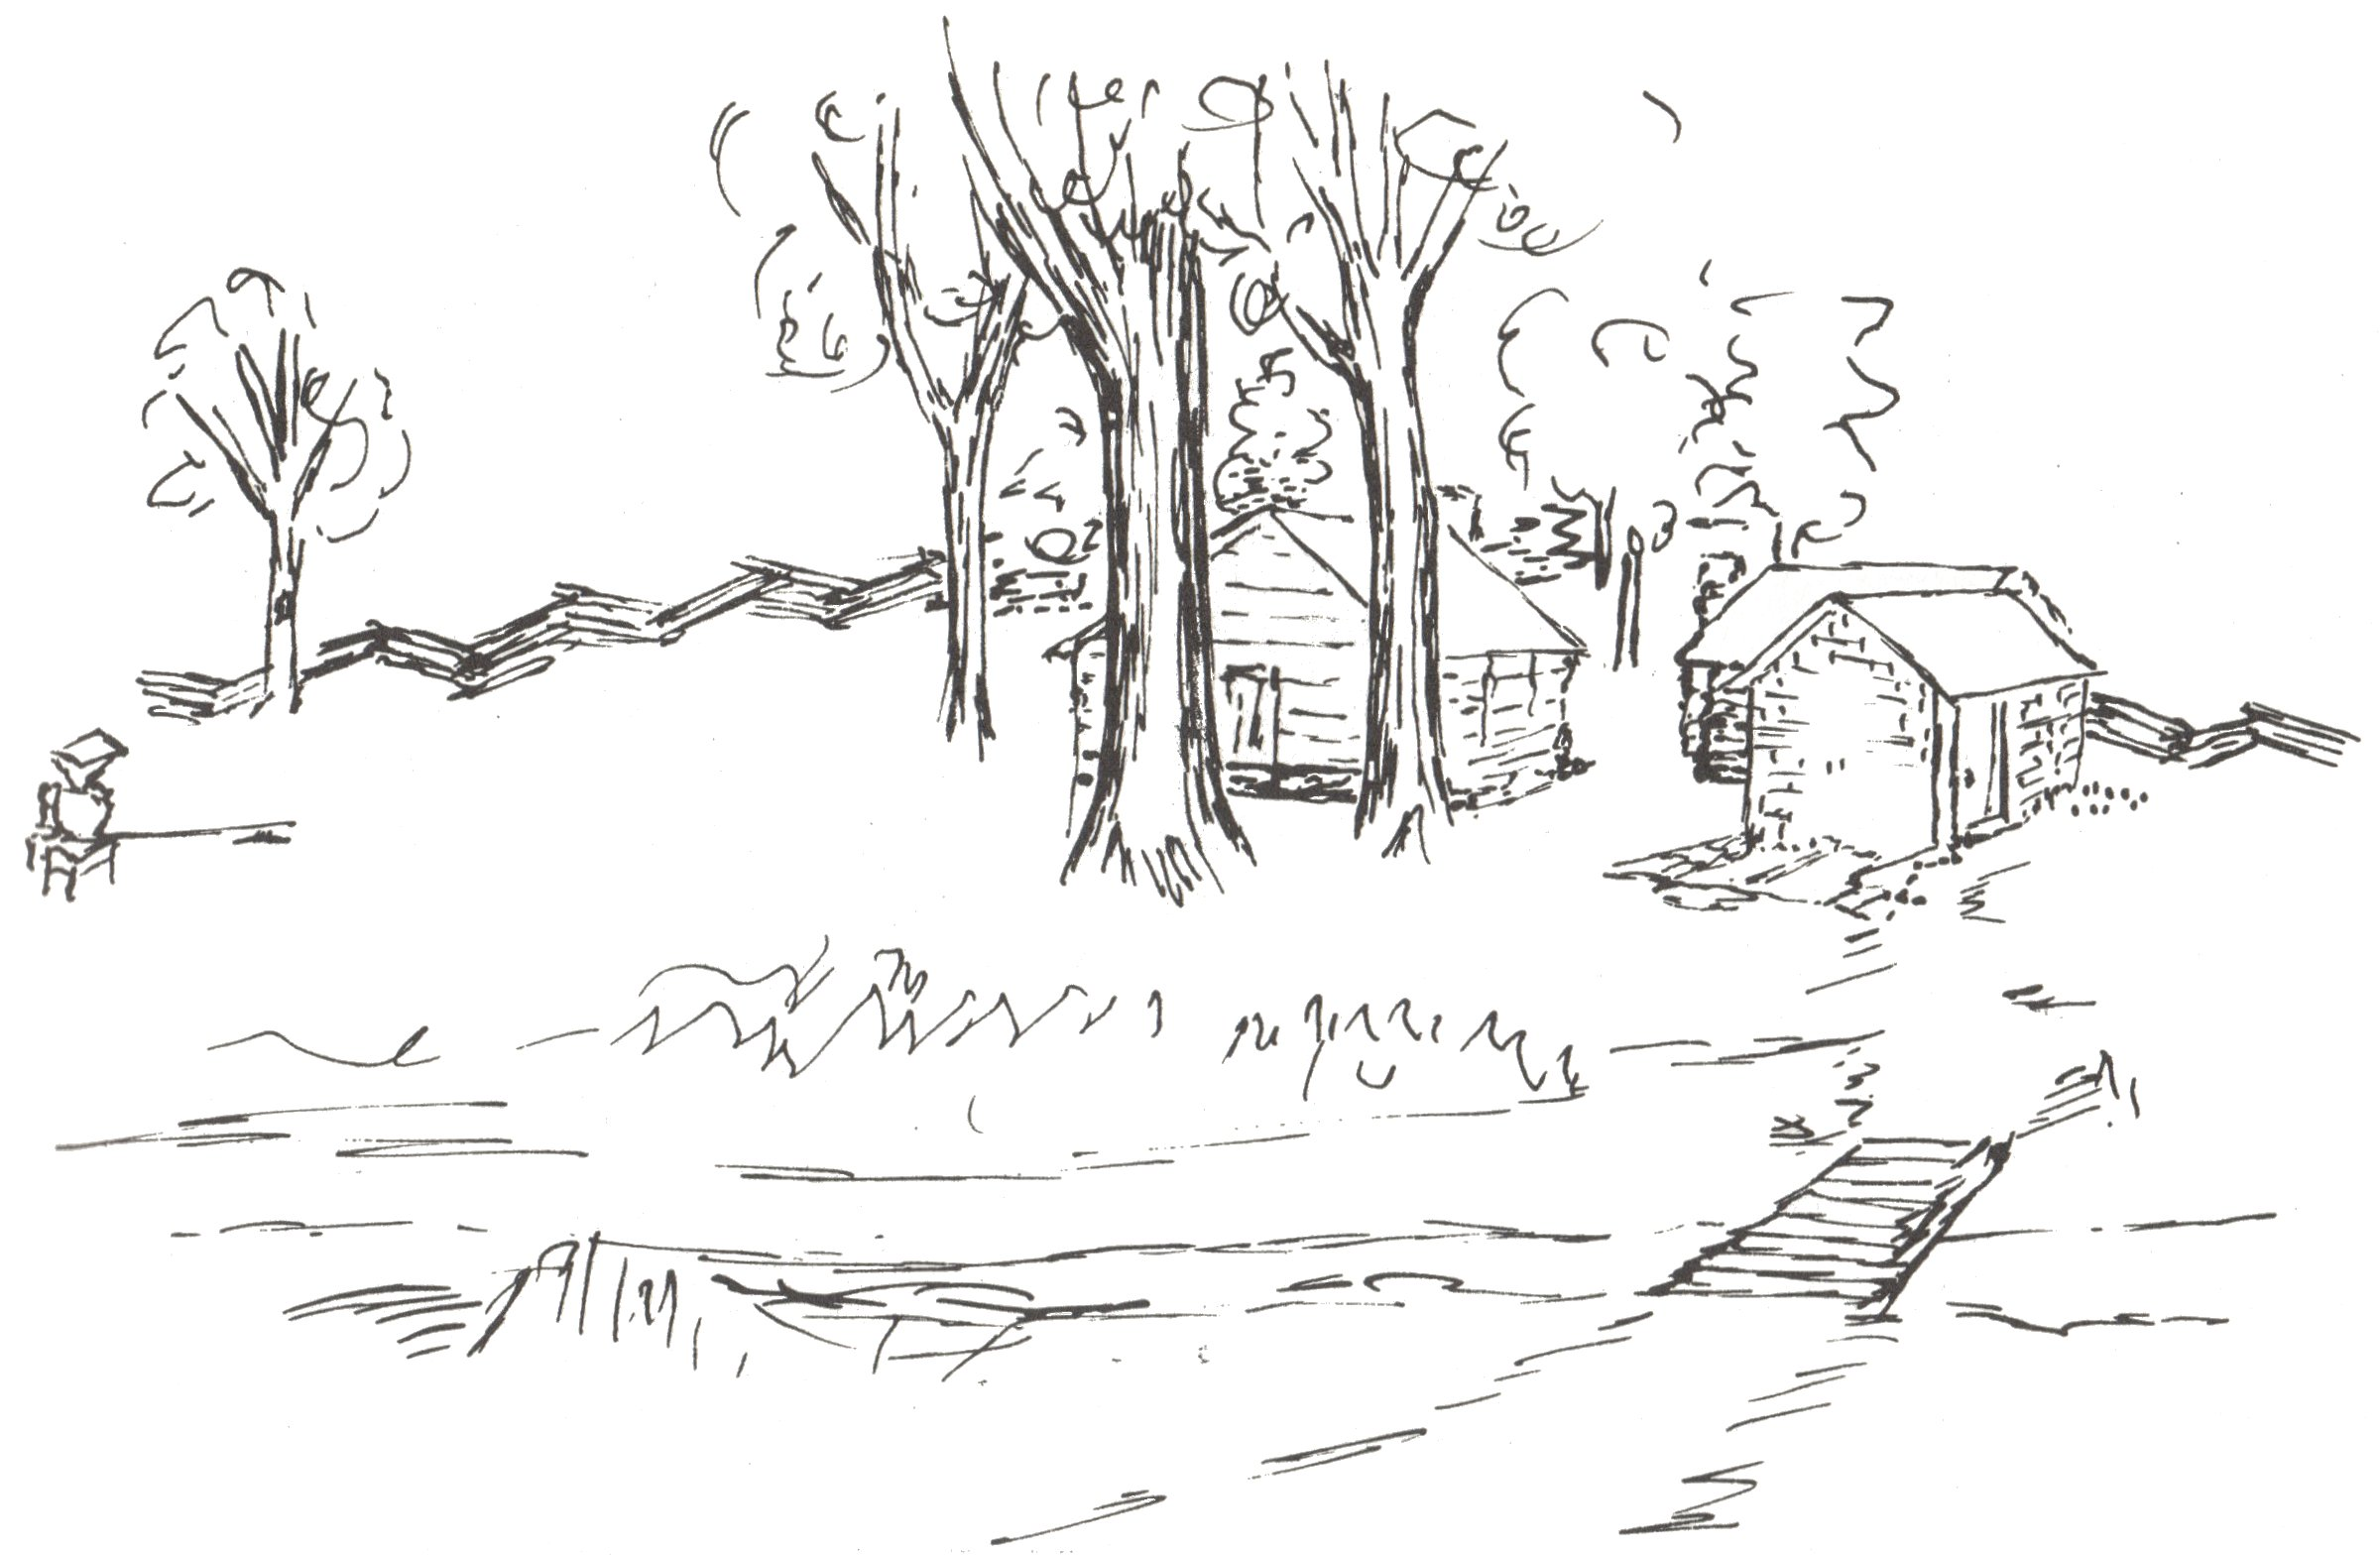
\includegraphics[width=.9\textwidth]{spring_area.jpg}
\label{}
\end{figure}

 

\section{The Spring}

 

The spring, the source of water for household use, was all of a long city block away.  It was located in a small grove of American elm trees.  The path to it lay just outside the yard on the kitchen side of the house.  It went past the servant's house and paralleled the creek to a group of weeping willows where it crossed on a plank bridge.

 

The spring itself was good and bold, and no doubt the Graves had chosen the house site because of it, but it had the serious disadvantage of being too near the creek and only slightly above it. Whenever thunder was heard it was thought wise to send a child running to put the milk and butter up on the shelf of the springhouse since the creek often got out of its bounds and flooded the spring and springhouse.  One rainy July the plank bridge was washed away three times.  There were two other springs on the place, on ``in the woods'' and one ``on the hill'' to supply water in these emergencies, but they were much further from the house and not as bold.

 

The spring had been improved.  It flowed from a small depressed area and this natural depression had been dug out and shaped into a neat square about eight feet in size and two and a half feet deep and walled with flat rocks.  Three stone steps led down into it.  The spring itself was also squared and lined with rocks.  A large flat capping rock was above it at the natural ground level, making the spring a little niche in the center of one side of the square.  It was deep enough and the capping rock high enough above it that a bucket could be filled by dipping without disturbing the crawfish and spring lizards at the bottom, or bumping the capping rock at the top.  A gourd dipper was kept there for the thirsty.

 

\section{The Spring House}

 

The spring house was built by Henry Brumfield himself, for he was good at carpentry.  It was ten feet square with walls of solid brick nine inches thick.  It had a gable roof with hand-split oak shingles.  Water from the spring flowed in a rock-lined sluice across the square from the spring and into the spring house through a small opening.  From the door, the only other opening, three steps led down to the brick floor.  Water flowed in a trough around three sides of the house.  Flat stones put here and there in the water made shallow places for bowls, crocks, and buckets were put in deeper places and watermelons and other fruits cooled on the spring house floor.  An emergency shelf high on the wall was the place to put things when flood threatened.

 

The spring water held a constant fifty degrees, and the house had a fresh, cool smell even on the hottest days.  This house was used for cooling foods as long as the spring was the source of water, and the only way for cooling them most of the time.  An ice-hole had once been dug for storing ice cut from the streams and ponds in winter, but it was not satisfactory and was soon abandoned.

 

\section{The Wash House}

 

The wash house, a squat log cabin, was located just behind the spring house.  The ground behind it rose sharply and had been excavated to make room for the house.  Thus the eaves on the back were near the ground and it was easy for children to scramble up on the roof and slide down its slope to a thrilling little jump to the dirt bank.  This was great fun, but hard on the seats of the pants.

 

Inside there was a good fireplace which furnished heat for the room in winter and heated water for washing the clothes.  This was done in a large three-legged iron pot on the hearth, and white things were boiled in this pot to keep them white.  There were benches for the wash tubs and corrugated wash boards for scrubbing.  There were pails for carrying water and a long wooden paddle for lifting the steaming clothes from the pot.  There were tables and shelves for supplies and even a chair or two in case the workers had a minute to sit down.

 

The washhouse also served as an extra kitchen at hog-killing time.  Soap was made there from waste grease.  Grandmother liked to make soap and some washwomen preferred the homemade kind to that from the store.  At one time the lye used in soap making was leached from wood ashes right there in the elm grove.  An ash hopper made of a hollow log stood there as a curiosity for years although this thrifty practice had become unnecessary.

 

The washing equipment was moved outdoors in summer.  Then the big pot was heated over an open fire, its legs propped up on stones, and the wash benches put nearby.  This custom led to a domestic catastrophe.  There had been a church meeting lasting three days at the Brumfield church and the house had been full of guests.  After the extra people had gone the two Negro washwomen put the piles of bed linen and Sunday clothes in the outdoor tubs to soak overnight.  During the night a flash flood washed them all away.  Some things were found and salvaged but were never white again, some things turned up moths later as barely identifiable relics, and some things were never found at all.

 

The labor of providing clean clothes for a large family was appalling.  First the laundress had to judge how to treat each piece.  White things were soaked and scrubbed and boiled and blued and starched.  Colored things apt to fade and run had to be handled separately and often separately from each other.  Washing clothes that a tobacco farmer had worn in the fields was not the simple job of removing heavy soil.  The tobacco plant is covered in fine hairs all over which exude a sticky gum.  This gum coats the workers hands and clothes with a dark green grayish mess that is extra hard to wash off.

 

Everything had to be ironed, even sheets and the baby's diapers.  Ironing was an art when starched wearing apparel trimmed with lace and ruffles was concerned.  The ironing was done in the kitchen with sad irons (a most appropriate name) which were heated on the cook stove.  It took five or six irons to keep a fast ironer supplied with one at the right temperature.  She took them from the stove in turn, testing their heat with a moistened finger.

 

\section{The Blacksmith Shop}

 

The third building near the spring was the blacksmith shop, and this was Henry Brumfield's particular pride.  It was a rectangle of logs with the gable end facing the elm grove.  The entrance was in the middle of this end.  When the opening for the door was cut the bottom log was left intact, running across the whole front of the building.  This strengthened the structure but all those entering, people and horses alike, had to step over it.

 

The roof was of split-oak shingles and the floor was packed earth.  There was a large fireplace at the end opposite the door.  A waist high general work bench extended the whole length of the shop on the left side, and a similar bench on the right ended in a raised bed of sand which held the forge fire.  This was a charcoal fire and a mounted bellows directed air to it fanning the charcoal fire until it burned white hot. This hot fire softened the iron so it could be cut and hammered into shape on the anvils.

 

In his shop Henry could shoe his own and his neighbors' horses and make and mend tools, chains, wheel rims and other metal necessities.  Several of his sons were good smiths too, particularly the youngest, and at least one horse was shod there as late as 1919.

 

The charcoal used was made in the woods and tell-tale pits could be found many years afterward.  There were many of these pits, for when the shop was in use much charcoal was needed.  Similar heaps of charred wood were the remains of another home manufacture.  Fat pine was burned in a covered smoldering fire to extract the pitch or pine tar.  This was used as a medicine to treat ailing animals.

 

\section{The Cider Mill}

 

There was a big black-walnut tree near the shop that played a part in making cider.  Children noticed this tree because it had a rectangular hole cut through its bole, and they wondered why.  Near this tree in a clear place outside the grove was the mill for grinding the apples.  It was turned by a horse that was hitched to a long shaft and made to walk around in a circle.  As the horse walked he turned the toothed grinding cylinders which ground the apples to a pulp as they were fed from the hopper above.  Any juice that drained off was caught and saved but the real extraction was in the press and this is where the walnut tree came in.  The press was a large wooden barrel with a plunger attached to a fulcrum, one end of which was supported by the hole in the tree.  The ground pulp was put in the barrel and when the fulcrum was pulled the plunger forced out the apple juice.  This time man power was used.

 

The cider made by this process was superb for no metal touched the apples.  There were formulae for arresting fermentation and holding a barrel of cider in the sweet stage which was a beverage, but most of the cider went to vinegar, a product of many uses.  Some hard cider was distilled to make brandy which was needed as a medicine and flavoring, and used as such even by people who abhorred it as a drink.

 

The walnut tree bore bushels of nuts.  Some of them were shucked and dried in a kiln and stored in the pantry to put in cakes and candy.  Later when the blacksmith shop was no longer a busy place the nuts were scooped up and thrown under the work bench in the shop where a child could get them whenever he wished.

 

 

\section{The Orchard}

 

Henry Brumfield gave his orchard much of his attention.  Apples were the most useful fruit, but the peach orchard was a thing of pleasure and pride.  Besides these a few cherry and pear trees had welcome fruit, and there were some currant and gooseberry bushes and grape vines.  Henry experimented with grafting and may have had success.

 

Before home canning of fruit in glass jars was developed fruit had to be pickled, brandied, or dried for preservation.  Drying made the most useful product, but it was an uncertain business, dependent on the whim of the sun.  Henry worked out a way to get around this.  He designed and made a fruit-drying kiln.  It worked like a tobacco curing barn but was a miniature.  It was about six feet high with slotted trays to hold the prepared fruit, resting on rows of tier poles.  The fire box at the bottom of the likn had a flue to release the smoke to the outside.  Gentle heat surrounded the fruit for a day or more, until the drying was complete.  Fruit dried relatively quickly this way and had better flavor and color.

 

[Sketch of farm buildings, with a bridge in the foreground straddling a creek]
\begin{figure}[h]
\centering
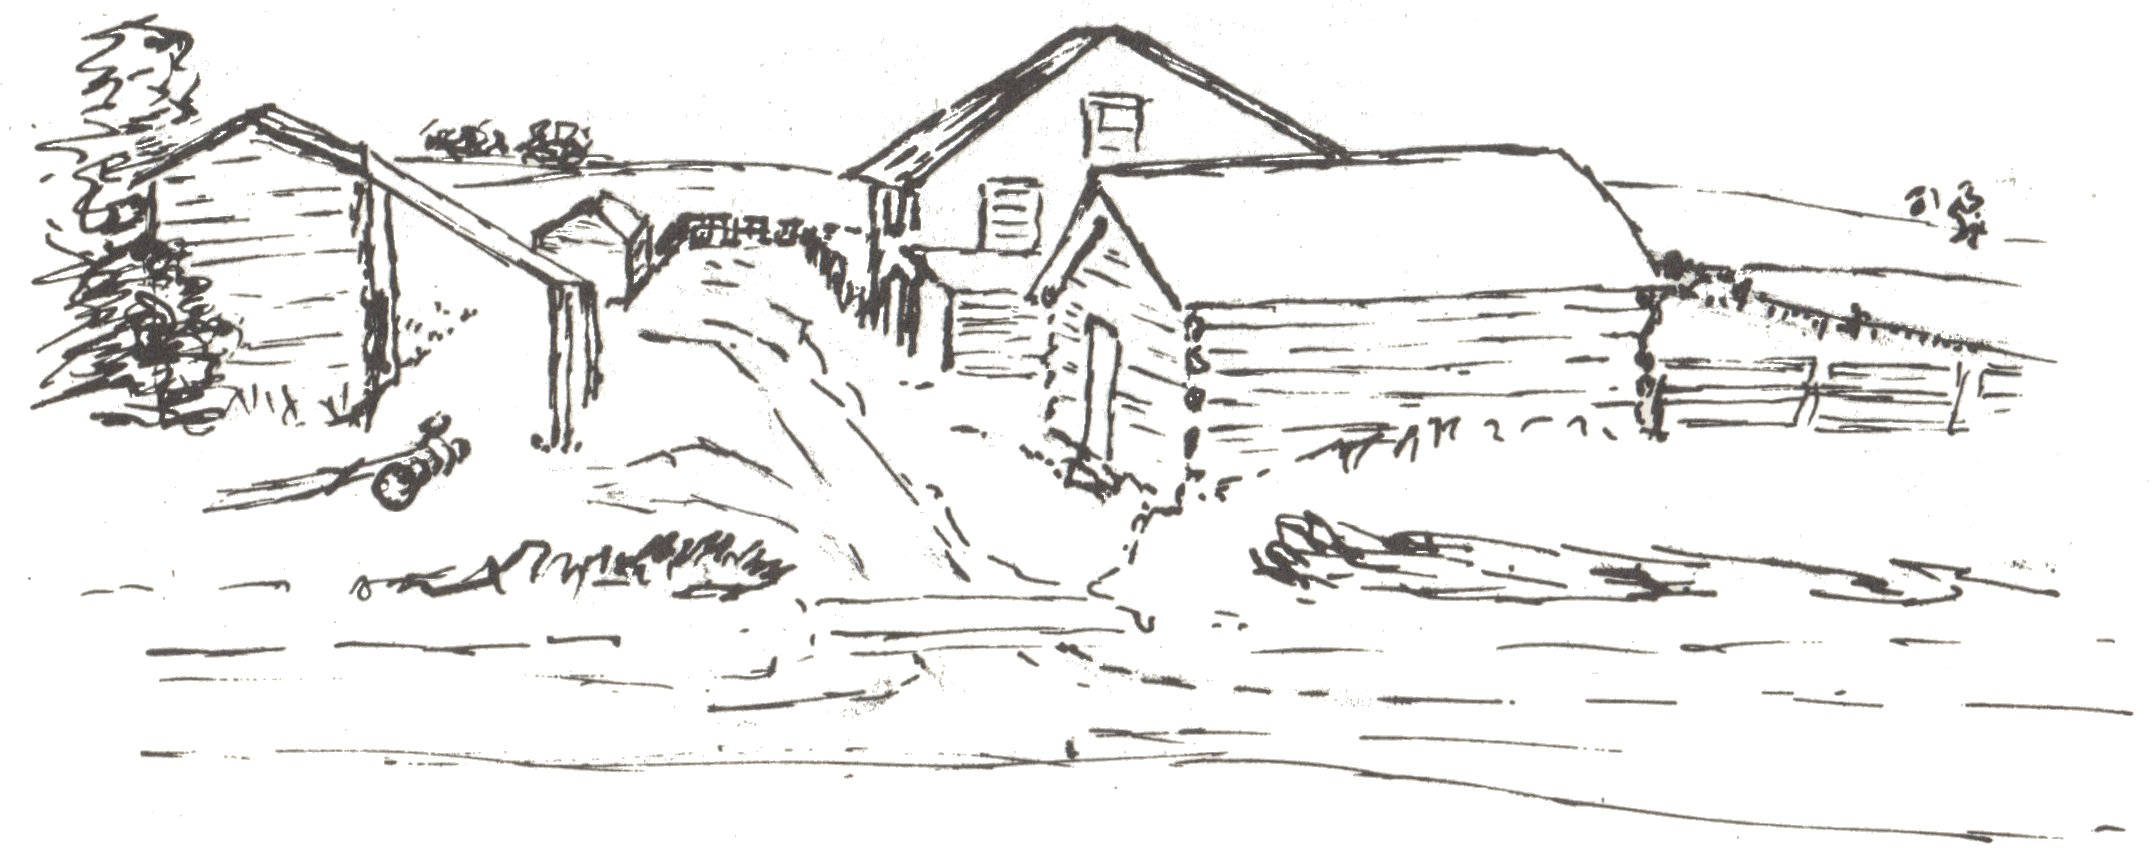
\includegraphics[width=.9\textwidth]{farm_buildings.jpg}
\label{}
\end{figure}

 

\section{Farm Buildings}

 

All the buildings so far listed, except the blacksmith shop, pertained to the house.  The real farm buildings were across the road.  The barn for horses with a harness room and hay loft, the cow stalls, the milking shed, the corn crib, the shelters for machinery and wagons, and perhaps some other structures stood in two rows on each side of a center ``street''.

 

Since this area was across the road it was not a usual play place, but it was interesting to visit.  Some young children loved to go with Grandmother when she did the milking, taking a tin cup to drink new milk warm and foamy from the cow.

 

Older children found it an exciting sport to knock down wasps' nests from under the eaves of these buildings.  The boldest advanced with a long pole to dislodge the nest.  Everyone was poised to run before the angry wasps could pinpoint the enemy, but they did not always make it.  Once a granddaughter was stung on the calf which swelled to twice its size.  She had a fellow sufferer in the little fox terrier, Cricket, who was stung on the jaw and had an enormous lump like mumps.

 

The horse and cow pasture was beyond the buildings.  The creek ran through this pasture and at one place it was dammed and widened to make a watering pond.  Children sometimes waded there, calling it ``swimming'', but Grandmother did not approve of this for it muddied the animals' drinking water.

 

 

[Sketch of a curing barn with wood stacked outside it]
\begin{figure}[h]
\centering
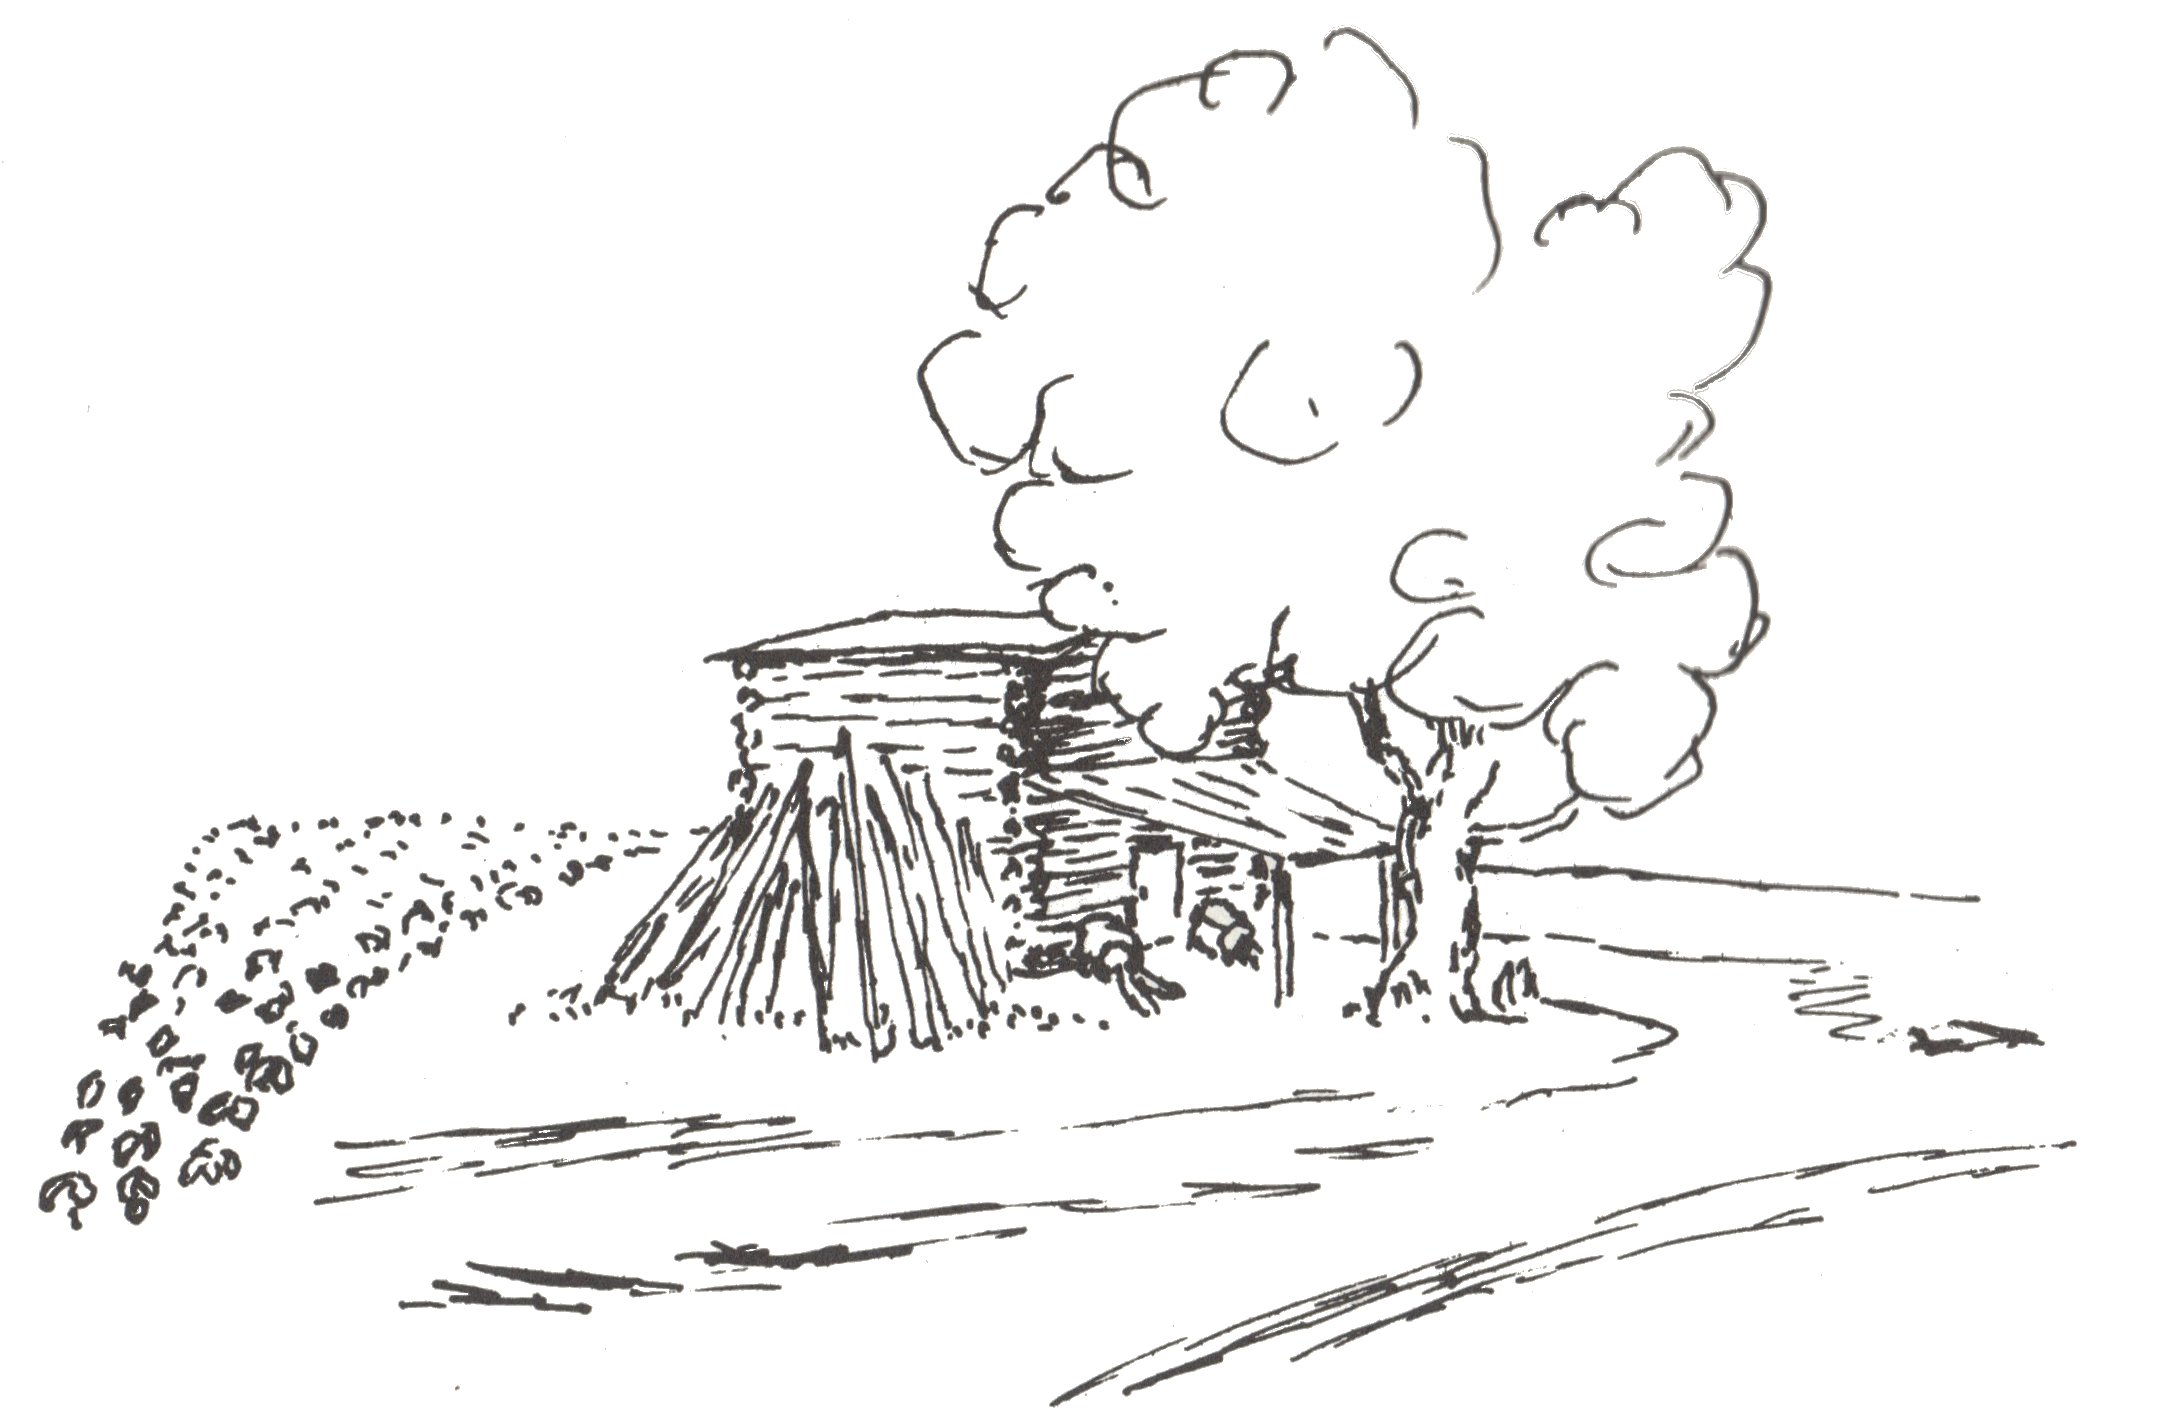
\includegraphics[width=.9\textwidth]{curing_barn.jpg}
\label{}
\end{figure}

 

\section{Tobacco Barns}

 

The most important farm buildings were for tobacco since it was the money crop.  The curing barns were in or near the growing fields.  They were rectangles with a square base about fifteen feet in size and some twenty feet tall (different barns varied in size).  They were built of logs, the spaces between the logs being chinked with rough strips of wood and daubed with red clay, making the sides air tight.  Ventilation was arranged in the roof.  The only opening was a door in the center of one side.  On most barns a shed ran all the way across that side.

 

Inside there were rows of tier poles crossing from front to back and reaching to the top of the barn.  They were spaced to be spanned by a tobacco stick.  A tobacco stick was about five feet long and of the thickness of a stout hoe handle (ideal for a child to ride as a play horse).  They were made by splitting a straight-grained tree trunk.  Stalks of green tobacco were hung over these sticks for curing.

 

Each barn had two fire boxes, one on each side of the door and opening under the shed.  They were long tunnels of stone about two and a half feet high and wide, reaching well within the barn.  They were connected with flues (the two flues might be joined) so that the smoke was released outside.  Wood to feed the fires was split logs and poles eight to ten feet long.  They were pushed into the barn as they burned, keeping the fires near the middle of the barn.  Wood for these fires was cut in the woods long ahead of curing time and stacked beside the barn so it would be well-seasoned by the time it was needed.

 

[Sketch of a stripping barn with a road in the foreground, and a tobacco field on the right]
\begin{figure}[h]
\centering
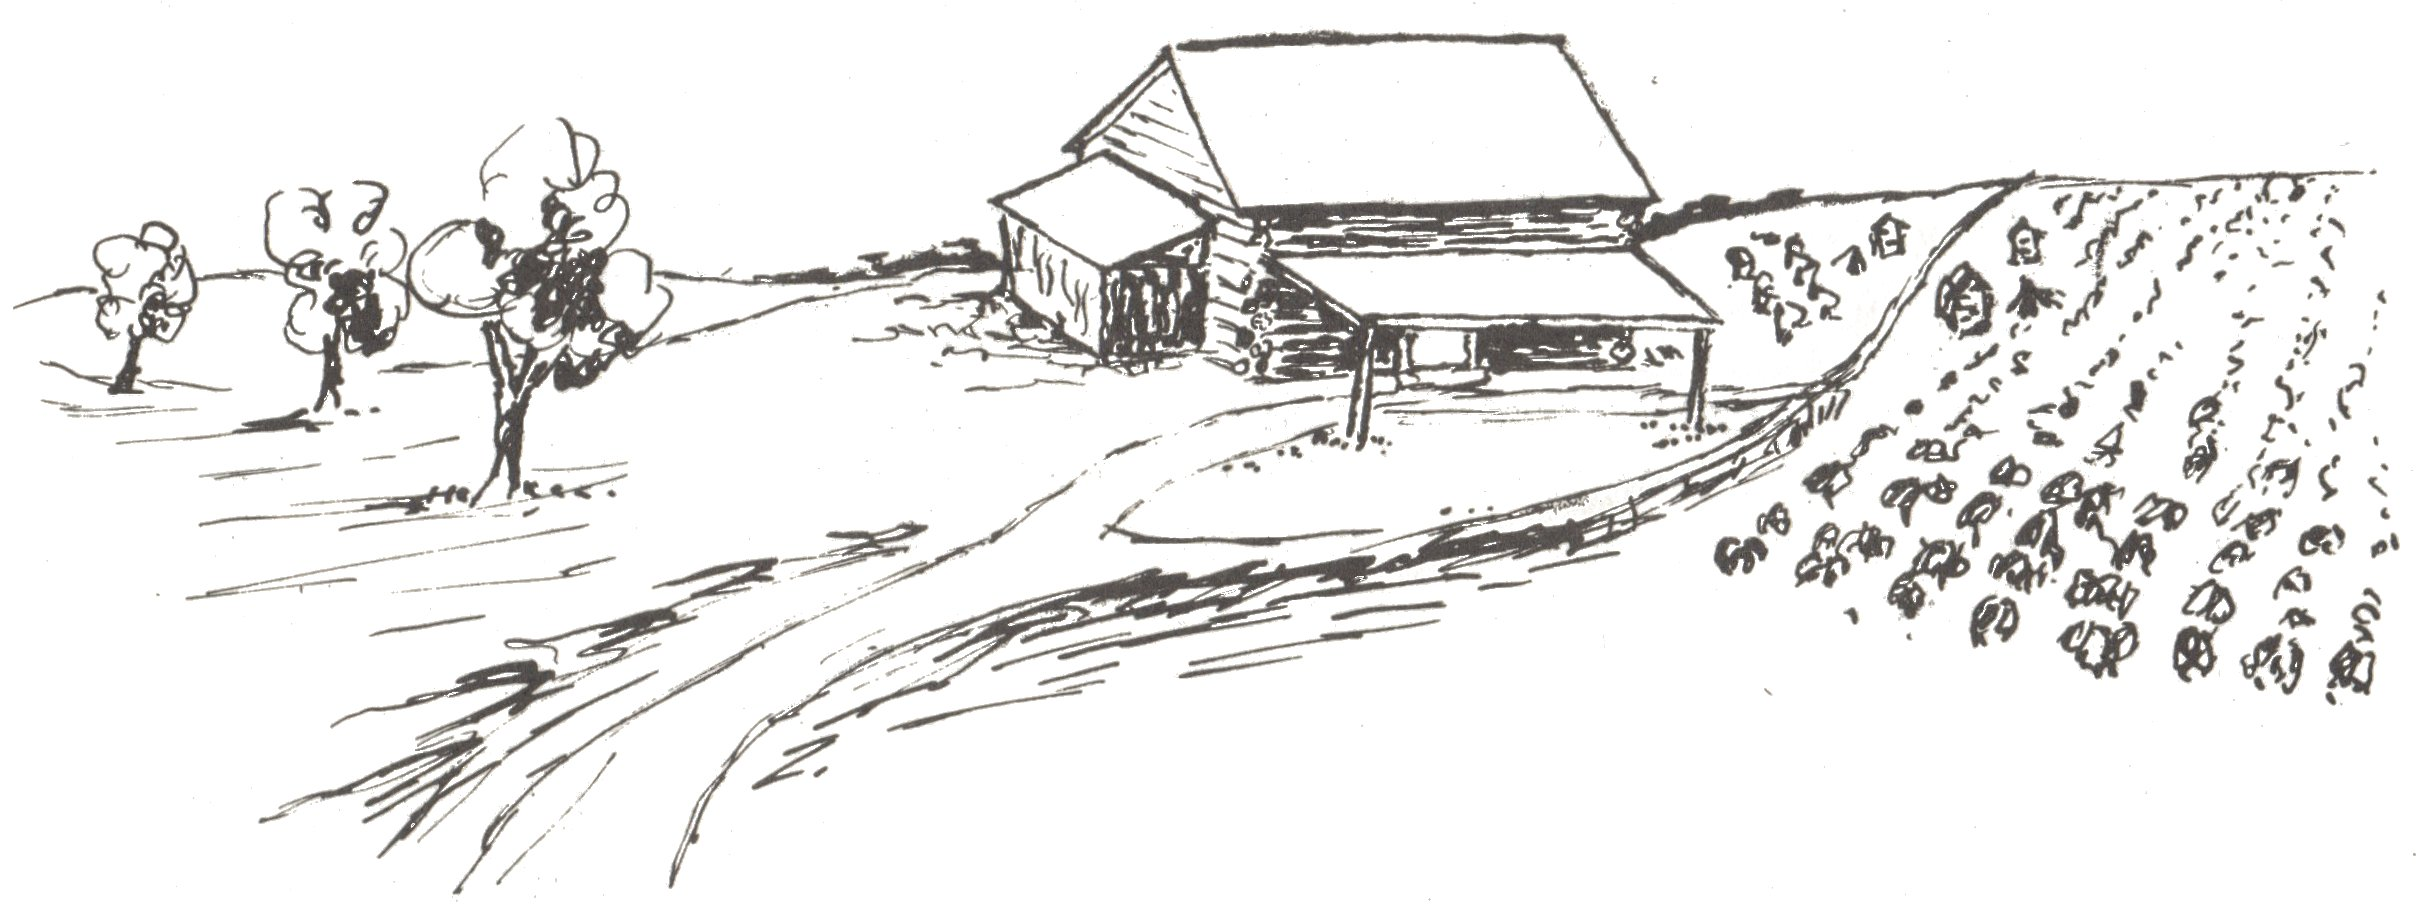
\includegraphics[width=.9\textwidth]{stripping_barn.jpg}
\label{}
\end{figure}

 

The stripping barn was of a different plan for a different purpose.  It was where the cured tobacco was prepared for market.  For convenience it was located on the main road and near the house, since work went on there all winter.  It had a heater for the comfort of the workers, storage rooms for the cured tobacco brought from the other barns, and an ``ordering pit'' to moisten the dry tobacco so it could be handled without crumbling.

 

 

\section{Tobacco Cultivation}

 

There was no month in the year that the tobacco farmer did not work on his crop, and all of this work was hand-work requiring great skill and judgment.  Seed beds were prepared in January; finishing with last year's crop in February; plowing, hauling guano and readying the fields in March and April; planting and re-planting the seedlings from the plant bed to the fields in May and June; topping, suckering and worming in late June, July, and August; cutting and curing in late August, September and October; stripping and marketing from November until March.

 

New ground, or newly cleared woodland, was best for the seed bed.  An area of about twenty by thirty feet was cleared, the stumps left standing, and the brush piled up and burned to partially sterilize the soil.  The bed was outlined with a border of logs.  After the seeds were planted the whole bed was covered with a plant-bed canvas stitched by the women folks.  It was made of thin unbleached muslin or �tobacco cloth� and was large enough to cover the whole bed.  It was tacked to the border of logs to keep the wind from blowing it off.

 

When the fields were ready and the weather was right plants were transplanted to the growing fields.  They were spaced wide apart, for althought tobacco seeds are tiny, as fine as dust, the cultivated plant grows over head-high and the ripe leaves may be two feet long and half as wide.  In the fields the plants were topped at about wasit level except for a few plants which were allowed to bloom and make seeds for next year.  The tobacco plant has pretty sweet-scented flowers of a lovely shade of pink.  The select plant chosen to make seeds produces an immense cluster of flowers as big as a water bucket and reaching to eye level or above.  The part of the stalk which reached above the height of the topped field was stripped bare of leaves so that the flower head resembled a little rose tree in a formal garden.  They were striking standing here and there in the field.  One such head would produce ample seeds, but most farmers grew five or six scattered about the field.

 

Topping the plants caused the growth of suckers in the axils of the leaves and the suckers had to be removed. Tobacco leaves ripen from the bottom and some farmers pulled one or two of the early ripened leaves from each stalk, tied them in bunches and hung them on tobacco sticks for curing.  A whole barn might be filled with these ``primings'' and fired, but many farmers skipped this extra work.

 

When the whole plant was judged ripe enough, the stalk was split from the top half way down and the plant cut off at the ground and hung upside down by the split crotch over a tobacco stick.  Holding sticks at tobacco cutting time was a job for a stout teen-age boy, or even a girl.  Each stick would hold six to eight plants, care being taken not to crowd them.  The filled sticks were placed on a wagon and hauled to the curing barn.  There they were hung between the tier poles, filing the barn from top to bottom.

 

Curing took several days of constant-temperature heat.  The farmer kept watch night and day during this process, checking the thermometer inside the barn frequently since well-raised tobacco could be ruined by poor firing.  Conversely, a poor crop if well cured brought a better price.  One of the Brumfield boys who was lazy about suckering made up for it by his great skill  at curing, to the envy and chagrin of his more industrious neighbors.

 

Children liked to visit the barn at night at curing time.  They liked to sit in the fire-light talking and eating potatoes roasted in the ashes and field corn and cornfield peas parched in their shucks and apples from a nearby tree.  Sleeping out seemed glamorous, but it was not so comfortable for the farmer.  He knew it as a time of very hard work.

 

Henry Brumfield was ever on the look-out for better and easier ways to do his work, and this trait passed to many of his descendants.  Because of it Brumfields call themselves lazy since they work so hard to avoid work.  Henry invented and had made to his specifications the first sheet-iron flues used in the county.  Another innovation was his ``ordering pit''.  To prepare the cured tobacco for market the leaves had to be stripped from the stalk and graded and tied into �hands� or bunches of like quality.  Bone dry cured tobacco was very brittle and could be handled without crumbling only in damp, muggy weather (when someone says ``tobacco weather'' that is what is meant).  When the tobacco was moved from the curing barn to the stripping barn the farmer had to wait for this misty weather since there was nothing else he could do, but when the tobacco was safely stored in the stripping barn Henry Brumfield figured he could do something.  He worked out a way of moistening his tobacco so that it could be handled whenever he wished.  This invention was his ordering pit.  His first one worked fine so far as making the tobacco fit to handle went but it was poorly ventilated.  After working there for a morning Henry and his helper were ``drunk'' from carbon monoxide poisoning and were lucky not to have passed out.  The flaw was corrected and the pits were generally adopted in the neighborhood. 

 

Julia always helped with the stripping and she was an expert grader.  Grading the tobacco was a very important step since how well it was done had much to do with the price received.  Stripping and grading was monotonous work, however.  Grandmother kept reminding herself that she was thankful for a large crop of good tobacco, but she longed to finish the dull chore so she could do more interesting things.  Wagon loads of tobacco were hauled to the buyers' warehouses a few loads at a time as they were ready, and selling went on all during the fall, winter and early spring.

 

[Sketch of a single horse pulling a covered wagon.]
\begin{figure}[h]
\centering
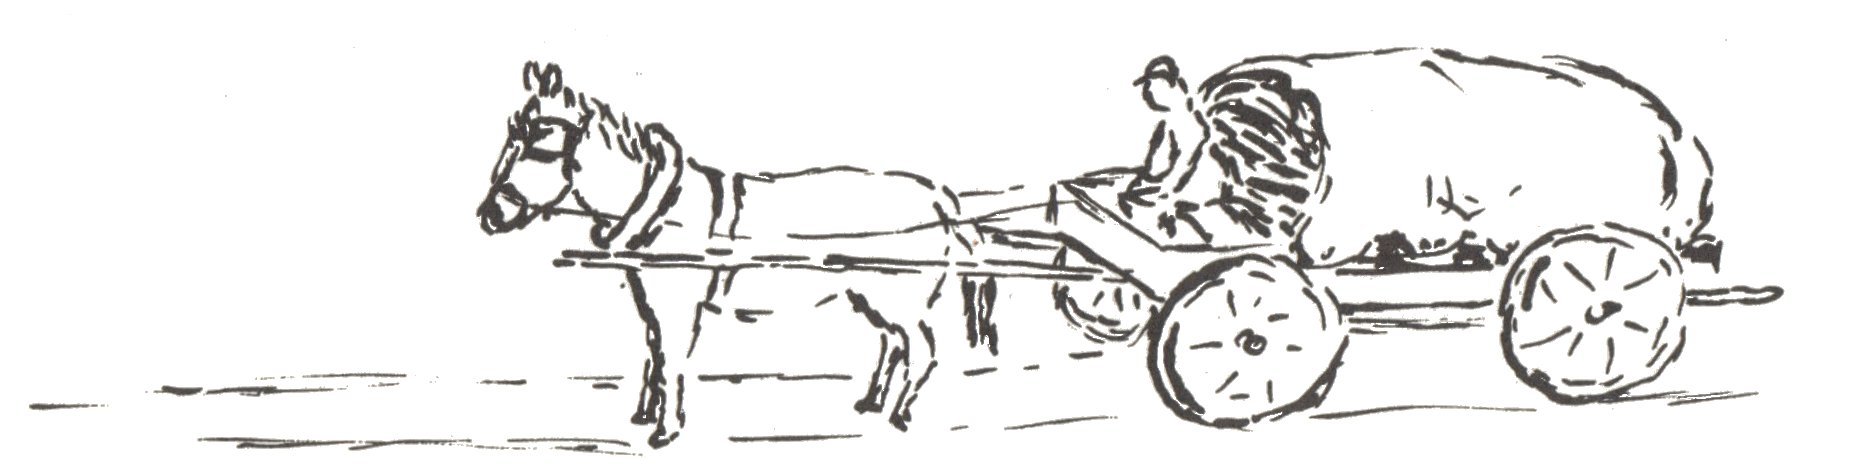
\includegraphics[width=.9\textwidth]{covered_wagon.jpg}
\label{}
\end{figure}

 

\section{Clothes}

 

Going to church and to the Association and to social affairs called for dressing up.   It was not beyond Julia's skill to make her husband's and sons' coats and pants.  She had done this in the early days using cloth that had been woven for her at the North Carolina mill from wool raised on the farm.  When ready-made suits at moderate prices were available she gave up this chore but continued to make their shirts, underwear and socks.  The socks were superior for she was an expert knitter.  She could managed four to six or more fine steel knitting needles and make beautiful small even stitches.  She kept her knitting in her apron pocket and worked at it whenever she had a few minutes to sit down, or she might even walk about and knit.

 

Julia and her girls made almost all of their own clothes, and their dress was smart by country standards.  They had an eye for line and color and they planned sewed and finished their clothes well and wore them with style.  According to some old diaries some sewing project was always under weigh, since it takes a world of dresses to keep so many girls well dressed.

 

Neatness in dress seems to have been a family trait since it is so often mentioned by those now living when asked to describe their elders.  In some this trait amounted to ``persnicketyness'' and made Grandmother most impatient.  One small son would never wear a garment with a loose or missing button, even going so far as to sew them on himself, which really was not a help.  Another would never work or walk where his shoes would get dirty if he could avoid it.  All the little boys were not like this, however.  There was one who never kept his shirt-tail in nor bothered to button buttons.  Grandmother lovingly referred to him as her ``Harum-Scarum''.  He thought this was a kind of compliment until one day he asked an older sister, ``What is a Harum-Scarum?''


\section{The Community �-- The Church}

 

There were few neighbors when the Brumfields first settled in the area, but other families soon moved in.  The elder daughters established households when they married and settled on their dower lands, and old Canada-land became a community.  The community's first need was a church.  Henry and his wife were Primitive Baptists, and Henry gave land and joined with a neighbor to build a church of this sect at Renan (the place had not been named at that time).  When the church was finished it was named ``Mt. Zion'' but some of the neighbors always called it the ``John-Henry'' because Mr. John Hodnett and Mr. Henry Brumfield had built it.

 

Such little churches did not have a resident minister.  With the bad roads services could not be held in winter, but an ``Association'' was held in summer to make up for it.  This was three or more days of special services, with morning and afternoon preaching by different visiting ministers and dinner on the grounds.  The whole neighborhood attended, members and non-members alike.  People from a distance were invited to spend the nights by those living nearby.

 

At one big Association at Mt Zion, Henry and Julia Brumfield had forty people staying in their house.  Grandmother bought bolts of unbleached domestic and sewed it into ticks and sheets.  She stuffed the ticks with wheat straw and they made quite comfortable beds no matter what floor they were put down on.  There were plenty of quilts for piecing quilts was a constant winter activity of the Brumfield girls.  (One winter they and their mother made fourteen and hope chests were full of them.)  These pallet beds were put in the parlor and loft of the carriage house as well as in the bedrooms.

 

Henry being equally mindful of his guests killed a beef and dressed several lambs.  Dozens of chickens were fried, many cakes and pies were baked and the store of pickles, jams and preserves was broached.  Other families vied with the Brumfields in providing good food for the dinners, and the picnic tables at the church were loaded with all sorts of delectable food.  People visited and sampled each other's specialties and housewives exchanged recipes.  Young people in their sub-teens gravitated together and made their own entertainment.  Serious courting was done by those a few years older, for the long, slow buggy rides to and fro offered excellent opportunity for this, and many a pledge was asked and given.  Friends met who had not seen each other for months.

 

The sermons were delivered inside the church, and were attended by young and old.  Some of the young would listen to only one sermon a day, but their devout elders heard them all.  At the close of every sermon there was an invitation to unite with the church and many answered the call.  A few days later the converts were baptized by immersion, and this rite was sometimes held in the stream on the Brumfield place.

 

The particular big Association with all the house guests was remembered as a super-happy time, but what fixed it even more firmly in mind was the flood which washed away the clothes that followed it.

 

 

\section{Schools}

 

Next to the church, a school was the most important need of the community.  When the family moved to the neighborhood the nearest school was at Mt. Airy about four miles away.  This was not regarded as too far to walk but the parents wanted one nearer.  Henry Brumfield gave the land and a new one-room school was built about a mile away to the south.  It was named Mt Harmony.  The young children and girls had an easy walk.  But Henry still sent the big boys to Mt. Airy because Mt. Airy had a man for a teacher.

 

When a beginner entered school his first assignment was to learn the alphabet by heart.  Until he could recite this to the teacher he was taught nothing else.  One of the Brumfield boys found this taks so dull he would not try.  He went to school a whole year (all of four or five months) without learning a thing.  Somehow he did learn to read the next year and was hooked.  All his life he had a book in his hand or in his pocket or at his elbow and he accumulated a sizeable library during his lifetime.

 

Henry and Julia Brumfield both felt that farming was the best life, and for this at that time ``higher education'' (meaning a college degree) was not needed.  They were school-minded people, however.  They sent their oldest son to Thompson's Military School in Siler City, North Carolina, for a school year. He wore a grey uniform trimmed in black braid and forty-four brass buttons which had to be polished.  He took honors in penmanship.  He learned to write in a flowing hand that looked well on the page and was easy to read, and also to do fancy writing.  In this style he could sign autograph albums with the letters shaded and decorated with swirls and flourishes, and he could draw a bird or spray of flowers without lifting his pen from the paper.  It was a good school and he was also taught more practical things.

 

The other boys might have had similar training if they wished, but the fourth son wanted more.  He wanted to go to the University of Virginia and study medicine.  When his parents were convinced this was a real ambition they were sympathetic but disturbed.  Henry thought it unfair to give one so many years of college (it then took two to three years to earn an MD) and not the others.  He got around this dilemma by lending the son the money on the land he planned to give him later.  Julia feared going to college would make the boy stuck-up and set him apart from his family.  There has always been a ``generation gap''.

 

The next younger brother thought he would follow the example of his brother.  He went to Richmond to study dentistry, but two days there was enough.  He did not like the food and was homesick.  When the youngest daughter had finished at the country school her father was old and sick and reluctant to send her away for more training, but Julia was determined this daughter was to have something more.  She financed a year at Blackstone Female Institute herself.  The mortar board and gown in which the graduate received her diploma hung for years in the back bedroom closet and was a favorite dress-up costume for theatricals.

 

\section{Parties and Amusements}

 

The young Brumfields enjoyed dancing and went to dances ten to fifteen miles away, even over the terrible roads in winter.  Written invitations were not given for anything so formal would hurt the feelings of those left out.  It was more diplomatic to let word go out that there would be a gathering at a certain home and friends and neighbors of all ages would come.  Young children were put to bed in their hostess's beds until the party was over.  Dancers were all the way from pre-teen to late middle age.  Later when evangelists preached that dancing was wicked and some neighbors and family members and in-laws felt strongly that this was so, few dances were given.  Whatever their own opinions, Julia and Henry Brumfield respected others' views and were careful never to offend if it could be helped.  They wanted peace in the neighborhood as well as in the family.  Party entertainment then turned to singing games.  It was all right to play Virginia reel but not to dance it.

 

The boys and girls played cards but their father hated cards.  He got this hatred in the army when it was his job to cook for his squad and the card-playing soldiers would not stop a game and come promptly to meals.  (This kind of indifference makes any cook mad.)  Henry did not forbid his children to play cards, he merely confiscated all decks left lying around.

 

Yard swings and croquet sets were enjoyed in summer.  There were sometimes organized outings like hayrides, picnics, ball games and tournaments.  In the tournaments the ``knight'' mounted on a horse and armed with a ``lance'' rode full tilt and tried to put his lance through a ring hanging from a tree limb.  It was not necessary to plan entertainment, however, since being with friends was the pleasure, and just visiting was entertainment enough.  When the host or hostess was busy the visitor would pitch in and help get the job done quicker while catching up on the gossip.

 

 

\section{Fishing}

 

Julia Craddock Brumfield loved to fish.  Some of her children also liked the sport, but it had little appeal for her husband, and her youngest son hated it.  These were the two men who headed her household for all of her long life.  Knowing their views, she disliked pressing them to go with her and it was hard for her to get in enough fishing.  She could fish for minnows in the Brumfield creek, but this was child's play and she was ashamed to be caught at it.  To fish seriously one had to go to the rivers and ponds.  When transportation was by horse and buggy she could hitch up and go whenever she wished (or her conscience would allow), taking a child or two as companions and a picnic lunch for all.

 

When automobiles came in Julia lost this independence.  Being over seventy she could not crank a car and never learned to drive.  Her son, often somewhat reluctantly, took her with him when he went to the grist mills or had errands near a pond or river.  He would leave her to fish while he transacted his business.  Sometimes on her birthday he would take her fishing as a present.  Unfortunately the fishing season coincided with the busiest time on a tobacco farm; a farmer could not get off just any old time to fish.  Julia knew this but she felt in her bones (and rightly) that being past seventy she had earned the right to fish as often as she pleased.  There was conflict in her mind, however, as well as with her son over this.  Before going on a fishing trip she would get up extra early and do her regular chores plus others with more diligence than usual so she could go with a clear conscience.

 

Some of her other children who liked to fish and grandchildren and neighbors often invited her to go fishing with them.  One grandson who was barely twelve years old and had to look through the steering wheel to see the road was a favorite companion and driver.  He was a careful, steady boy and like all farm boys grew up knowing how to make things go.  No one thought him incapable because he wasn't.  Traffic on the road was no problem, the car could not go fast enough for speed itself to be a danger.  Blowouts, punctures (this problem was once solved by filling the tire casings with solid rubber), balky engines and mud holes and ruts too deep to pull out of were hazards but life was not in danger from them.  Most of these short trips came off successfully, however.  The two would fill the car with other grandchildren who would wade or play if they did not care to fish.

 

One year, by her own count, Grandmother averaged nearly two fishing trips a week during the season, but her idea of enough fishing was to go every clear day.  When she woke up to a beautiful morning with a blue sky and fresh inviting air she longed to be on a river bank.  She had always been so independent that she had to steel herself to ask someone to take her, and it hurt to be denied.

 

[Sketch of woman fishing]
\begin{figure}[h]
\centering
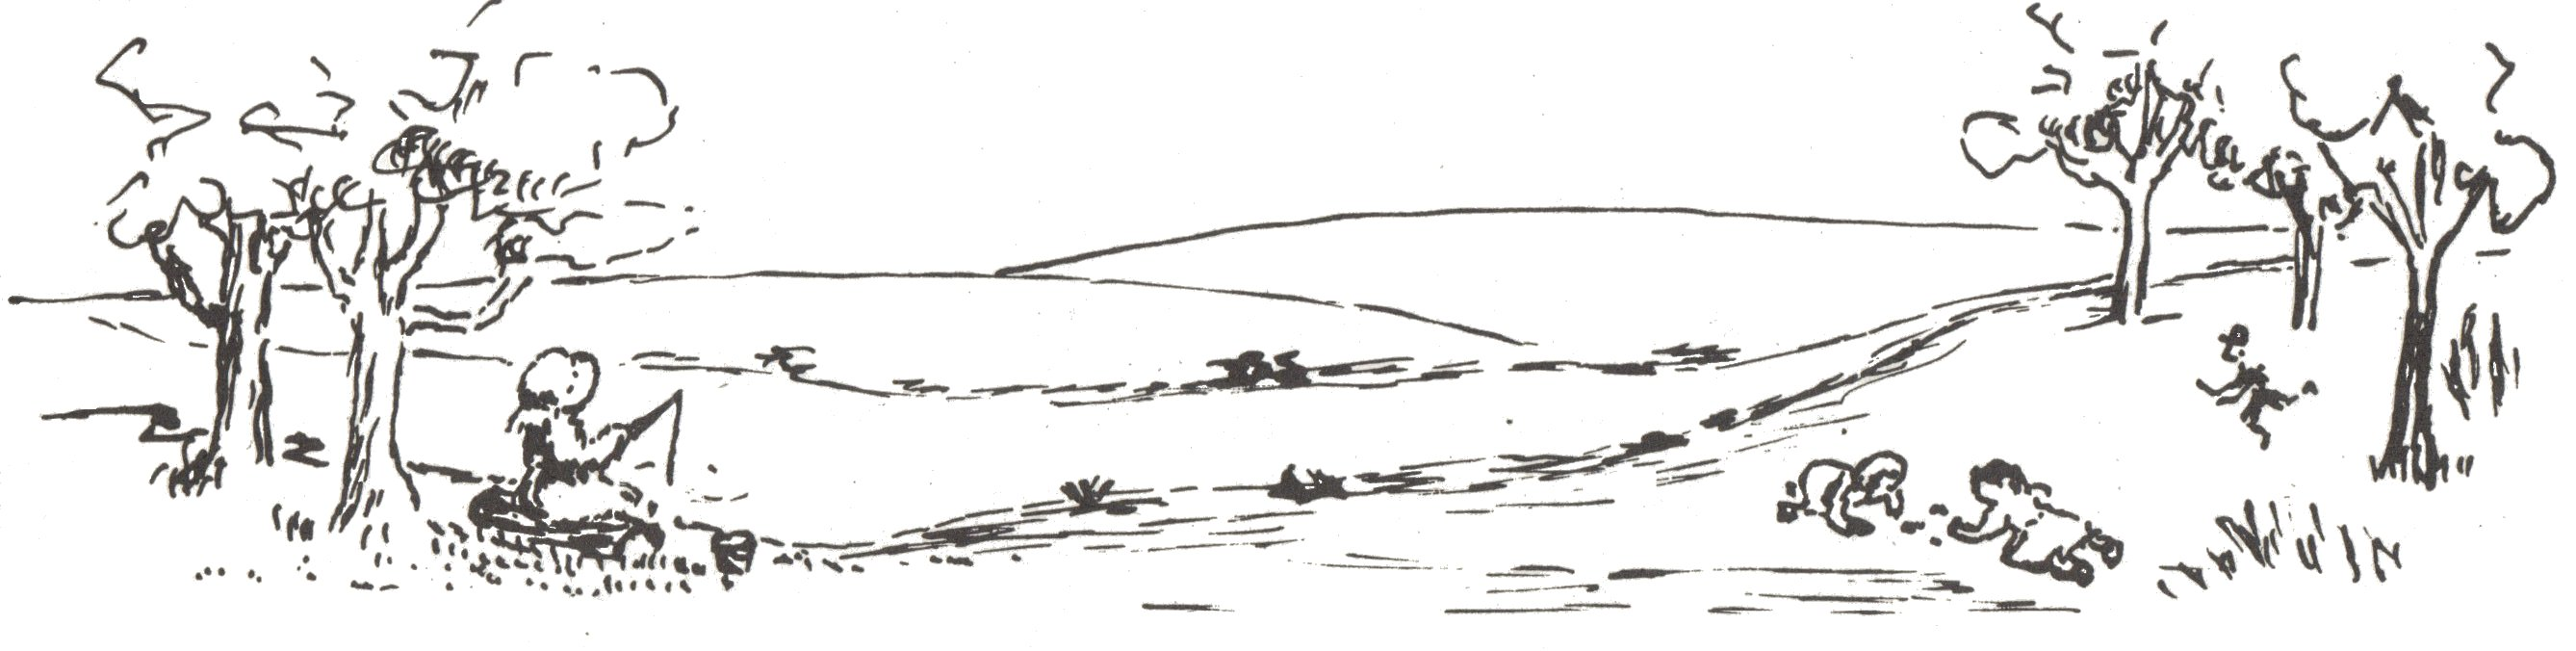
\includegraphics[width=.9\textwidth]{woman_fishing.jpg}
\label{}
\end{figure}

 

 

\section{Renan}

 

The son who was a doctor came back from medical school and practiced in the neighborhood.  With his father's help he built a store on the land his father had given him and they petitioned successfully for a post office there.  The post office had to have a name and the son chose to call it ``Renan'' after a French philosopher and humanitarian whose writings he admired.  Neither the young doctor nor anyone else in the neighborhood spoke French, so the name was accented on the first syllable as in English.  Renan is still on the map and the store is still in business but it is no longer a post office.

 

The store faced the main road from Mt. Airy to Altavista and was located at a fork where the road to Henry Brumfield's farm and to Straightstone branced off.  It was an attractive setting in a grove of big trees with a good spring nearby.  The original building was a thrity-by-forty foot two-storey frame structure with the narrower gable end facing the road.  Double doors opened in the center and there were two big windows, one on each side of the door.  Inside, shelves and counters ran along both side walls and a pot-bellied stove stood in the middle on a bed of sand.  This stove was a focal point for neighborhood news.  The customers sat around it on chairs, benches and boxes and exchanged views of crops, hunting, politics and local happenings.  Smokers and chewers used the sand box as a spittoon to the dismay of whoever had to clean it.

 

Upstairs there were three windows on each side of the building, all with functional outside blinds.  This floor was used at times as living quarters for some of the storekeepers and it made a comfortable and attractive home.

 

The timber used in building the store was cut from the original forest and the counters and shelves of long, wide, straight boards are in good condition and still in use.  There have been changes in the main structure, however.  A thirty by thirty addition was made at the back, and when the road in front was straightened and moved too far from the front door a new front was made on that end.  The store now faces the Straightstone road.  The old porch was torn down and a new porch built for the new front and no steps were needed here because the ground level is higher.  A long storage shed has been added on the right and no one lives upstairs.  Ownership of the store has changed several times, but for a long time now the husband of one of the Brumfield granddaughters has been the proprietor.  Their home is nearby, built on the spot where old Mt. Zion church used to stand.

 
\begin{figure}[h]
\centering
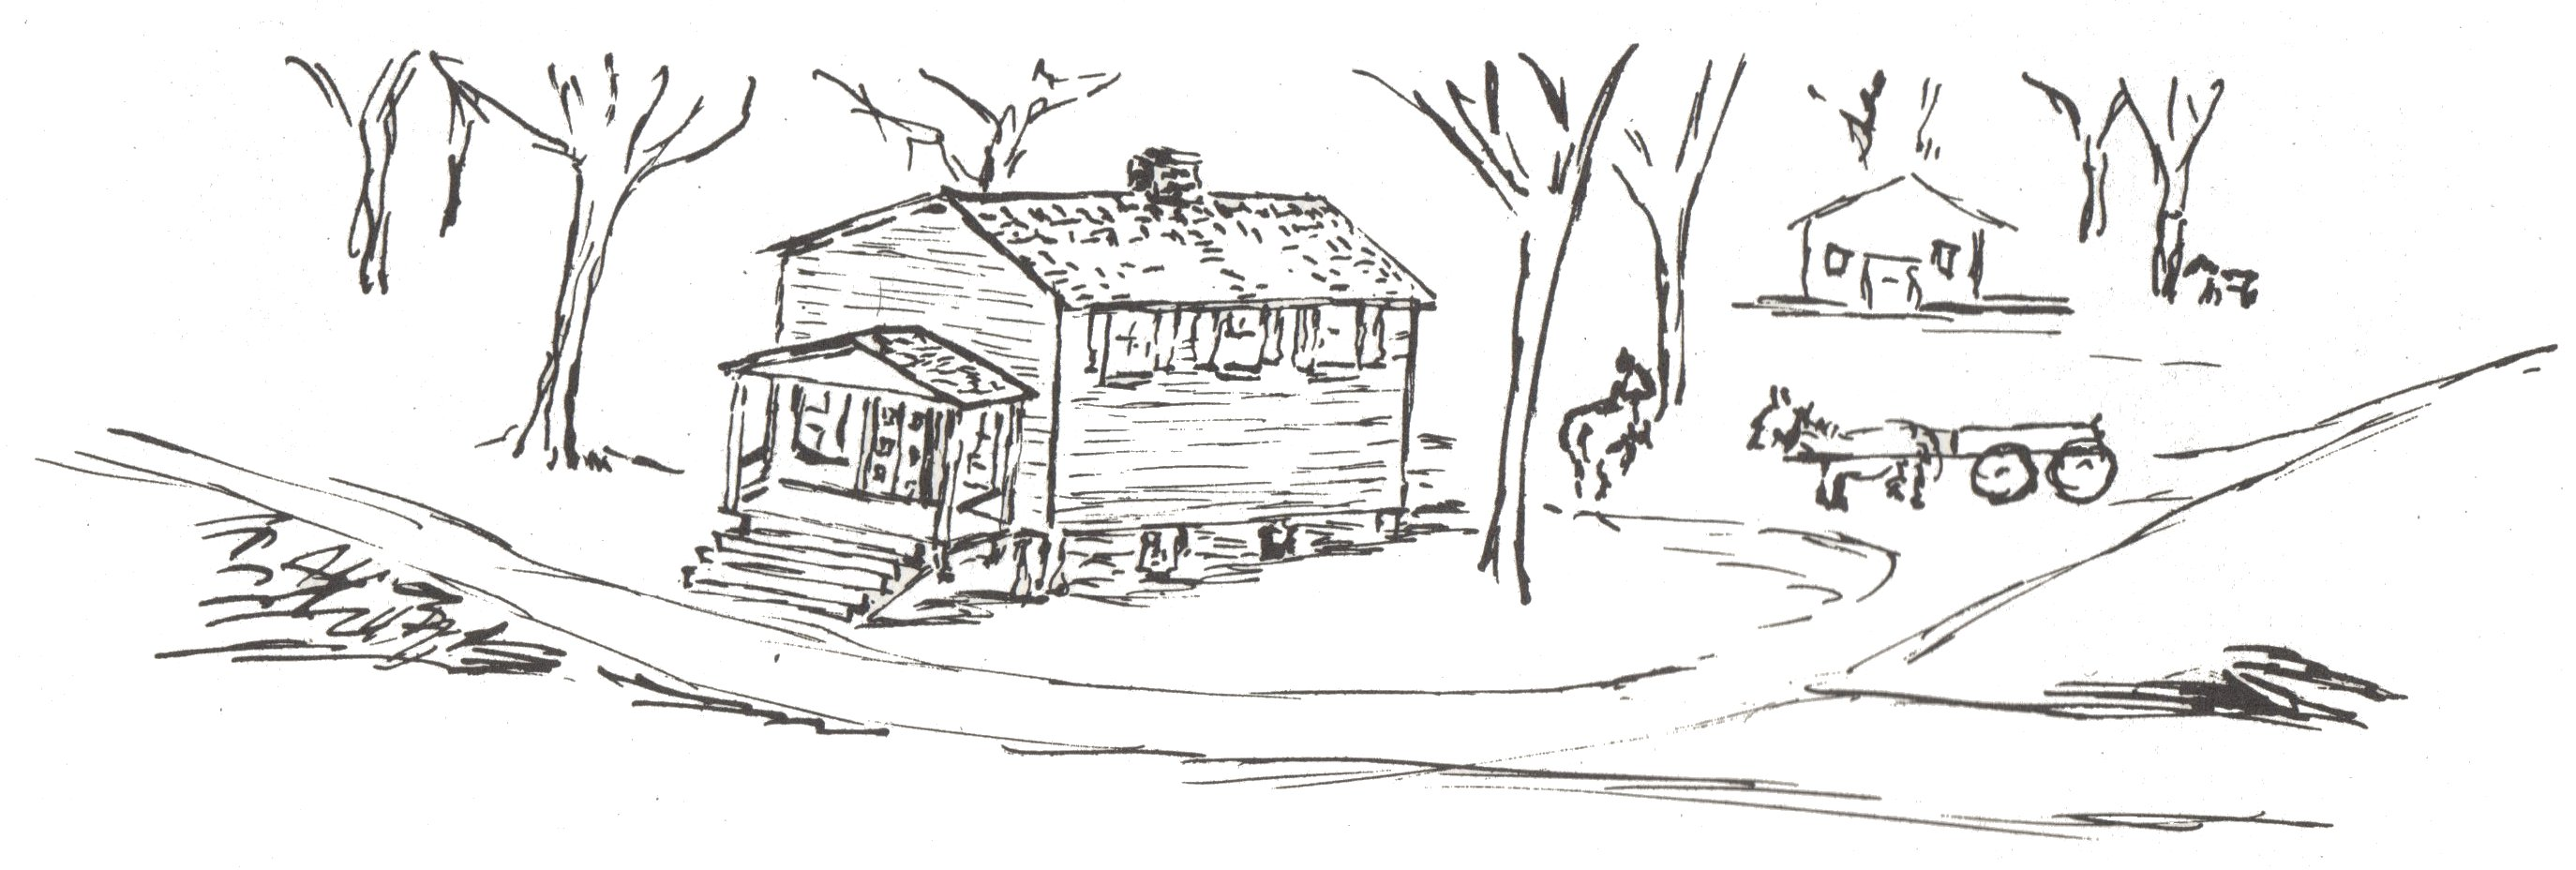
\includegraphics[width=.9\textwidth]{renan_store_sketch.jpg}
\label{}
\end{figure}
[Sketch of the store]

 
\section{Politics}
Candidates for County offices came to the store to shake hands and ask for votes and politics was a subject for discussion there.  No doubt Henry Brumfield took part because he was a thoughtful voter, but he never became more ative in politics than to serve as judge at election time.  He was a staunch Democrat.  Young men who called on his daughters were earnestly asked if they were Republicans and if they were they were not wholly approved no matter what other fine qualities they had.  All of his sons-in-law passed this test, but his niece whom he had raised as a daughter chose to marry a Republican.  It grieved him but in spite of this he and Julia gave the couple a pretty wedding in their parlor and were always happy to welcome them and their children as visitors.

\section{Realized Ambition}
Henry Brumfield lived to see nine of his children married.  Before the first wedding he marked out the hundred-acre parcels and tagged them for the different ones.  He hoped that all would settle and farm their acres and he let this hope be known but this wise and understanding father did not try to force is will.  His gifts had no strings attached and the recipients were free to swap with each other or to sell to each other or to sell to outsiders.  Much exchanging was done.  One daughter asked to be given land in another locality instead of at Renan and her father arranged it for her.  Another swapped with a brother who wanted to sell his parcel and she preferred his to hers because it had a house on it.

Most of the farms had buildings of sorts on them.  A sawmill company had cut timber on Henry's land in the nineties. They had built shacks and other structures for their hands, and the Brumfield children could camp in these and live on their own land right away.  A place to live while a house was being built was a necessity.  Building a new house of wood was not the instant thing of giving an order to a contractor and moving in in three or four months.  When kiln-dried wood was not available the custom was to dig and build the foundation one year, erect the framework of joists an dstuds in teh next year and let this skeleton season in place a year or two before putting on the roof an dsiding.  Only in this way could warped floors and cracked plaster be minimized.  The skeletons of houses in progress stood stark and ugly all that time and the wives looked at them with impatience.  Husbands could be more detached, and one of the Brumfield boys took years finishing a handsome addition to his house.  The addition had the new front door and even after the new rooms could be used for a long thim there were no front steps.  The big front door opened to nowhere, and all coming and going was at the back.  His happy and tolerant wife did not seem to mind, nor did his children and guests.

[Photograph of a small home on the south side of the Renan/Straightstone road]

Many of the newly marrieds lived in the sawmill shacks as their first homes.  The first daughter to marry kept house in a barn while a good house was being built.  Two of the unmarried boys and a neighbor's son set up bachelor's quarters and farmed their land for a season or two until the Brumfields married and built for their brides.  Thus, several of the older grandchildren can boast of a birthplace of romantic humbleness.

 

When the early shifting of titles was over there were seven households on the gift acres, six of them in the Renan community, and these families stayed on their land during the rest of their father's lifetime.  (Five of the children lived out their lives on their farms.)  During his last years Henry Brumfield would visit his children in turn, taking gifts of produce from his garden, orchard or pantry.  If Julia was not too busy and he was going by buggy she would accompany him, but if the roads were bad he would go alone on horseback.  Often he would bring grandchildren home with him for overnight visits, because he loved them and wanted to know them all.  This warm contact with his descendants was the fulfillment of his dream.

 

 

\section{The End of their Lives}

 

Both Henry and Julia Brumfield enjoyed good health for most of their lives.  Henry suffered a stroke in 1902 which left him completely paralyzed for some weeks, but he made a partial recovery.  He never regained movement in one arm, but he was able to drive to Renan for the mail in good weather.  Julia did not like for him to take the trip alone, but she was willing for a young child to be the companion.  One young grandson who visited there one summer enjoyed these daily trips immensely.  When he returned home he begged to go somewhere.  His mother explained he could not expect to go somewhere every day.  He cried, ``Mother, Grandpa has ruined me!''

 

Henry Anderson Brumfield died on April 21, 1905.

 

 

Julia Craddock Brumfield lived thirty-four years as a widow.  Her health was excellent until she had a stroke in 1937.  She got better but had lost much of the use of her hands.  She was advised to do hand-work to aid their recovery.  She could not begin to approximate her former exquisite stitches, but dutifully set about knitting wash cloths of cotton string.  The work is crude with many dropped stitches.  This poor work may have been because such work bored her, and she did not think anybody wanted the product anyway.  Thinking that working with bright colors would be more interesting to her, a son sent her yarn to knit an afghan.  He chose the loudest, most clashing colors he could find.  His mother's comment was, �He must be out of his mind!�

 

For a long time before her death Grandmother was confined to her bed and only semi-conscious.

 

Julia Craddock Brumfield died on September 17, 1939.

 

 

Henry and Julia Brumfield are buried side by side in the family cemetery at the Renan farm.
\begin{figure}[p]
\centering
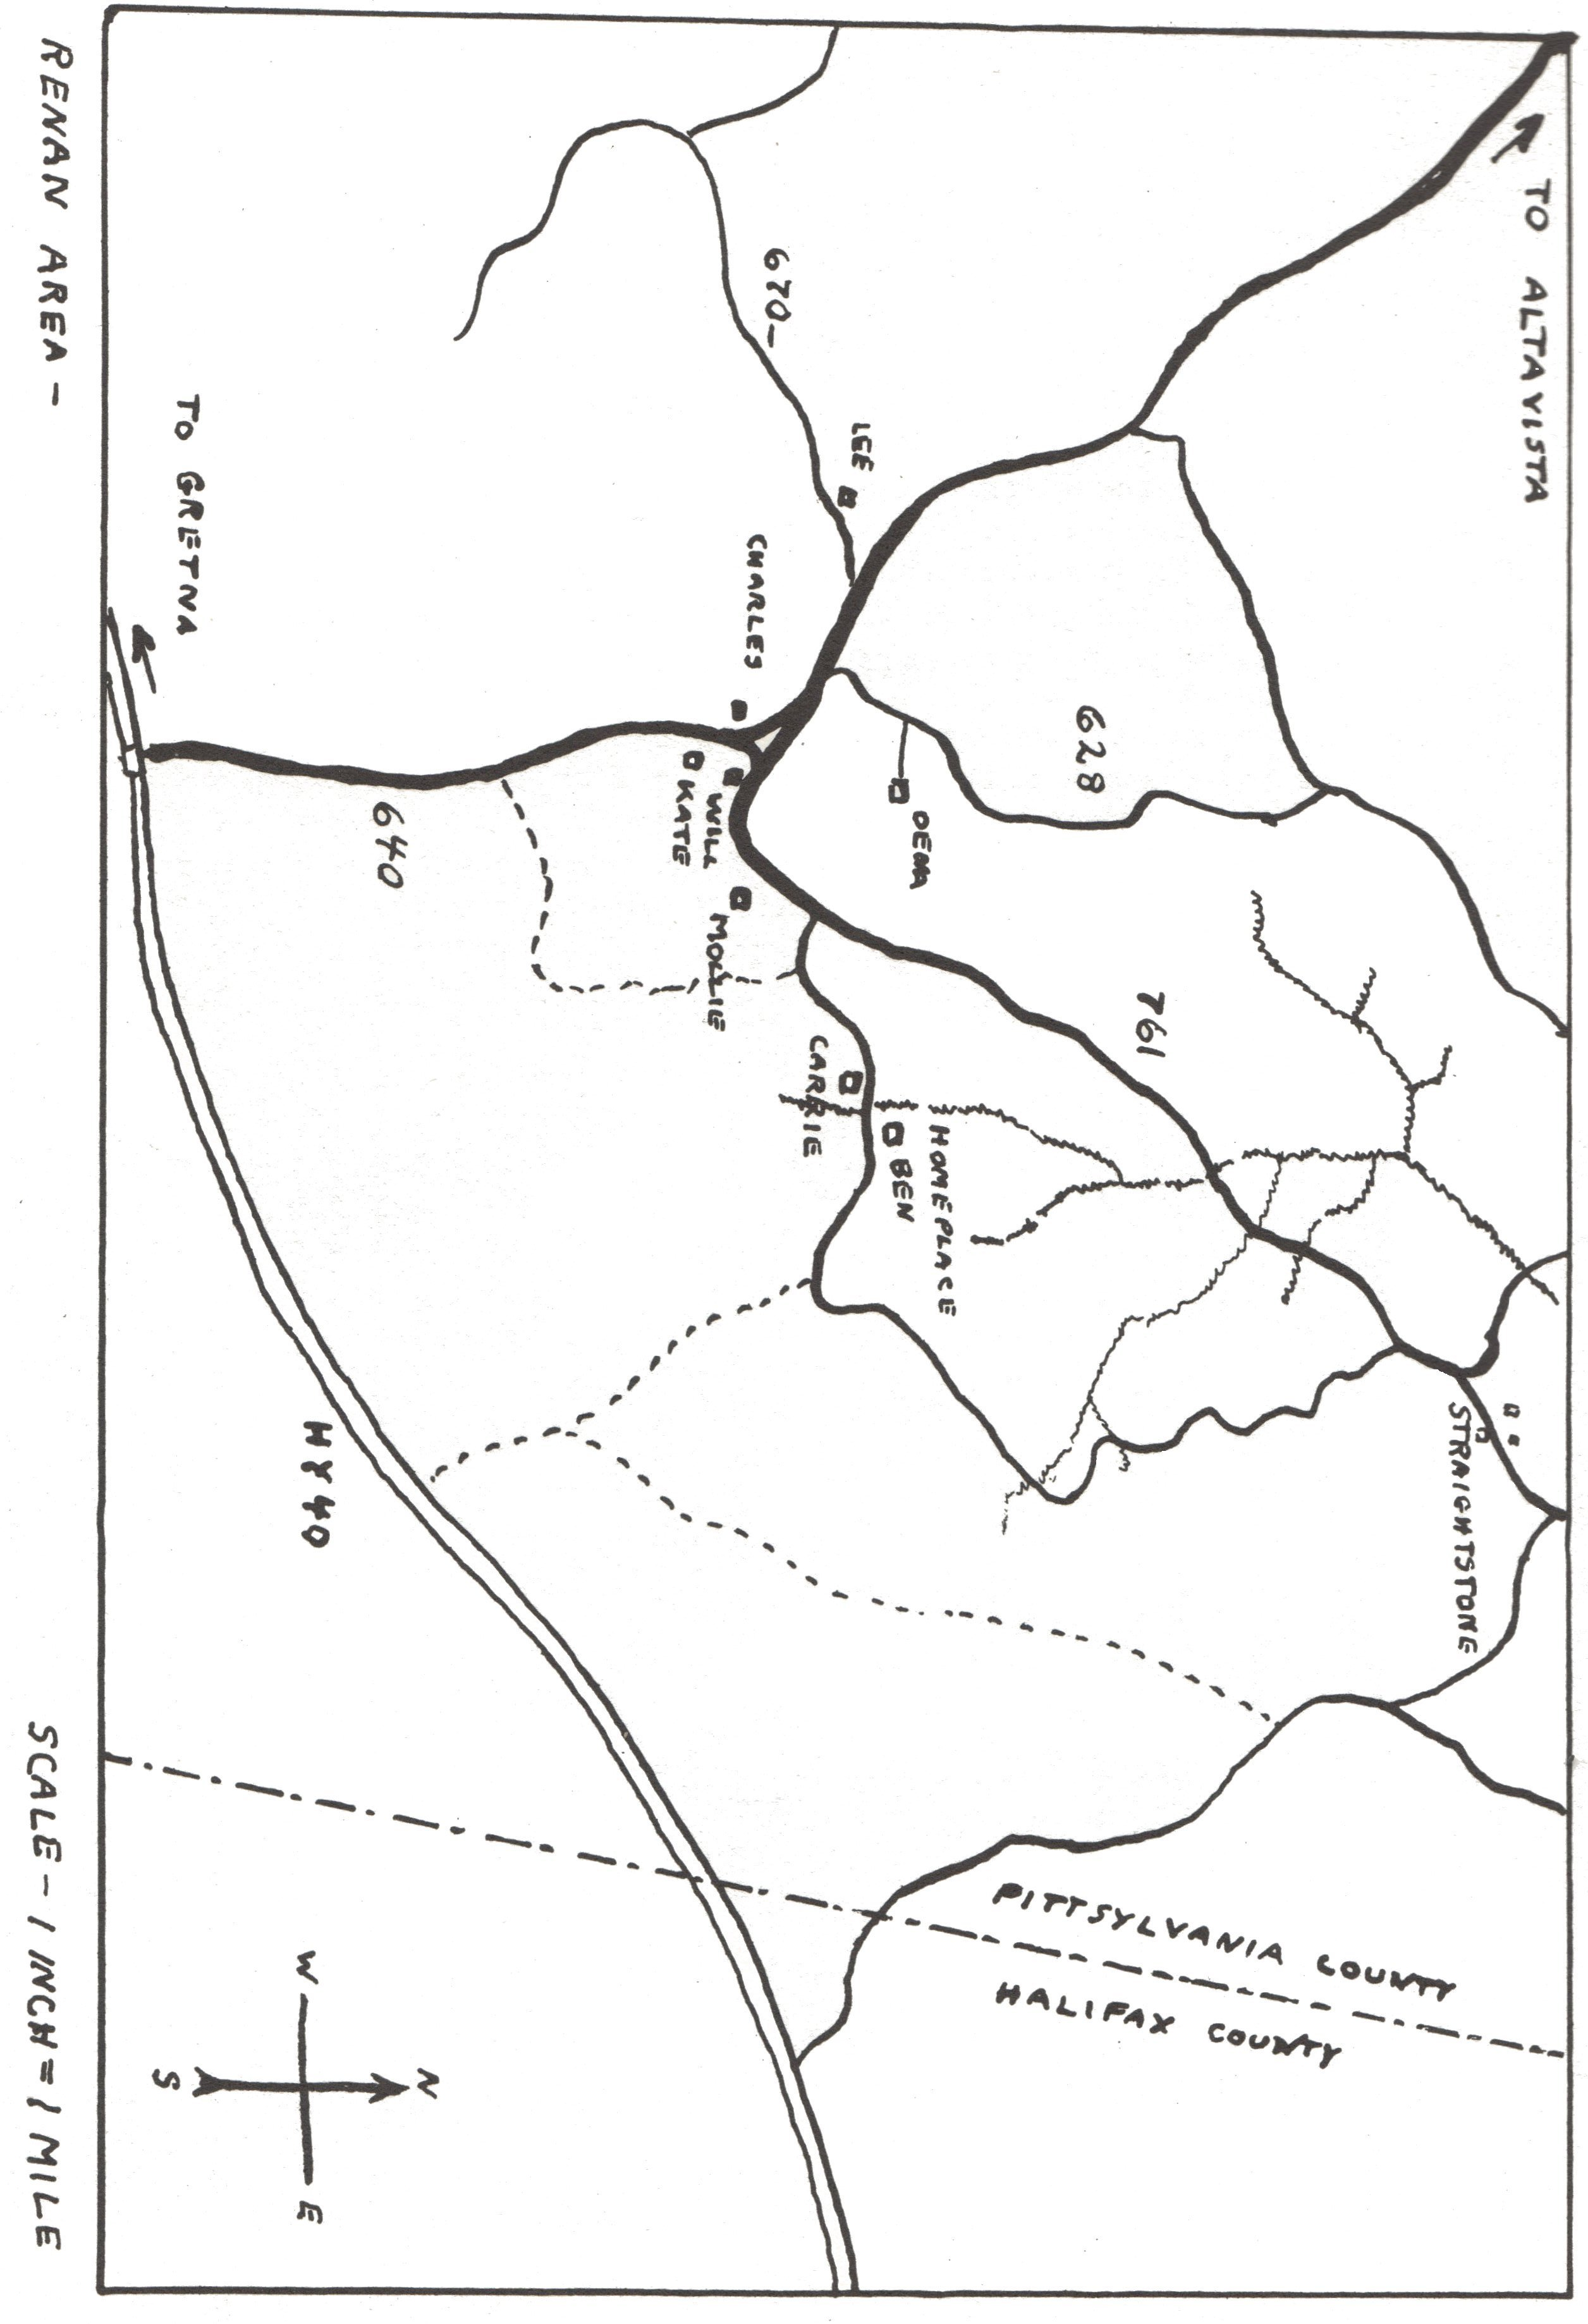
\includegraphics[width=1.0\textwidth]{renan_map_rot_90.jpg}
\label{}
\end{figure}

%[Map of Renan]
\begin{figure}[p]
\centering
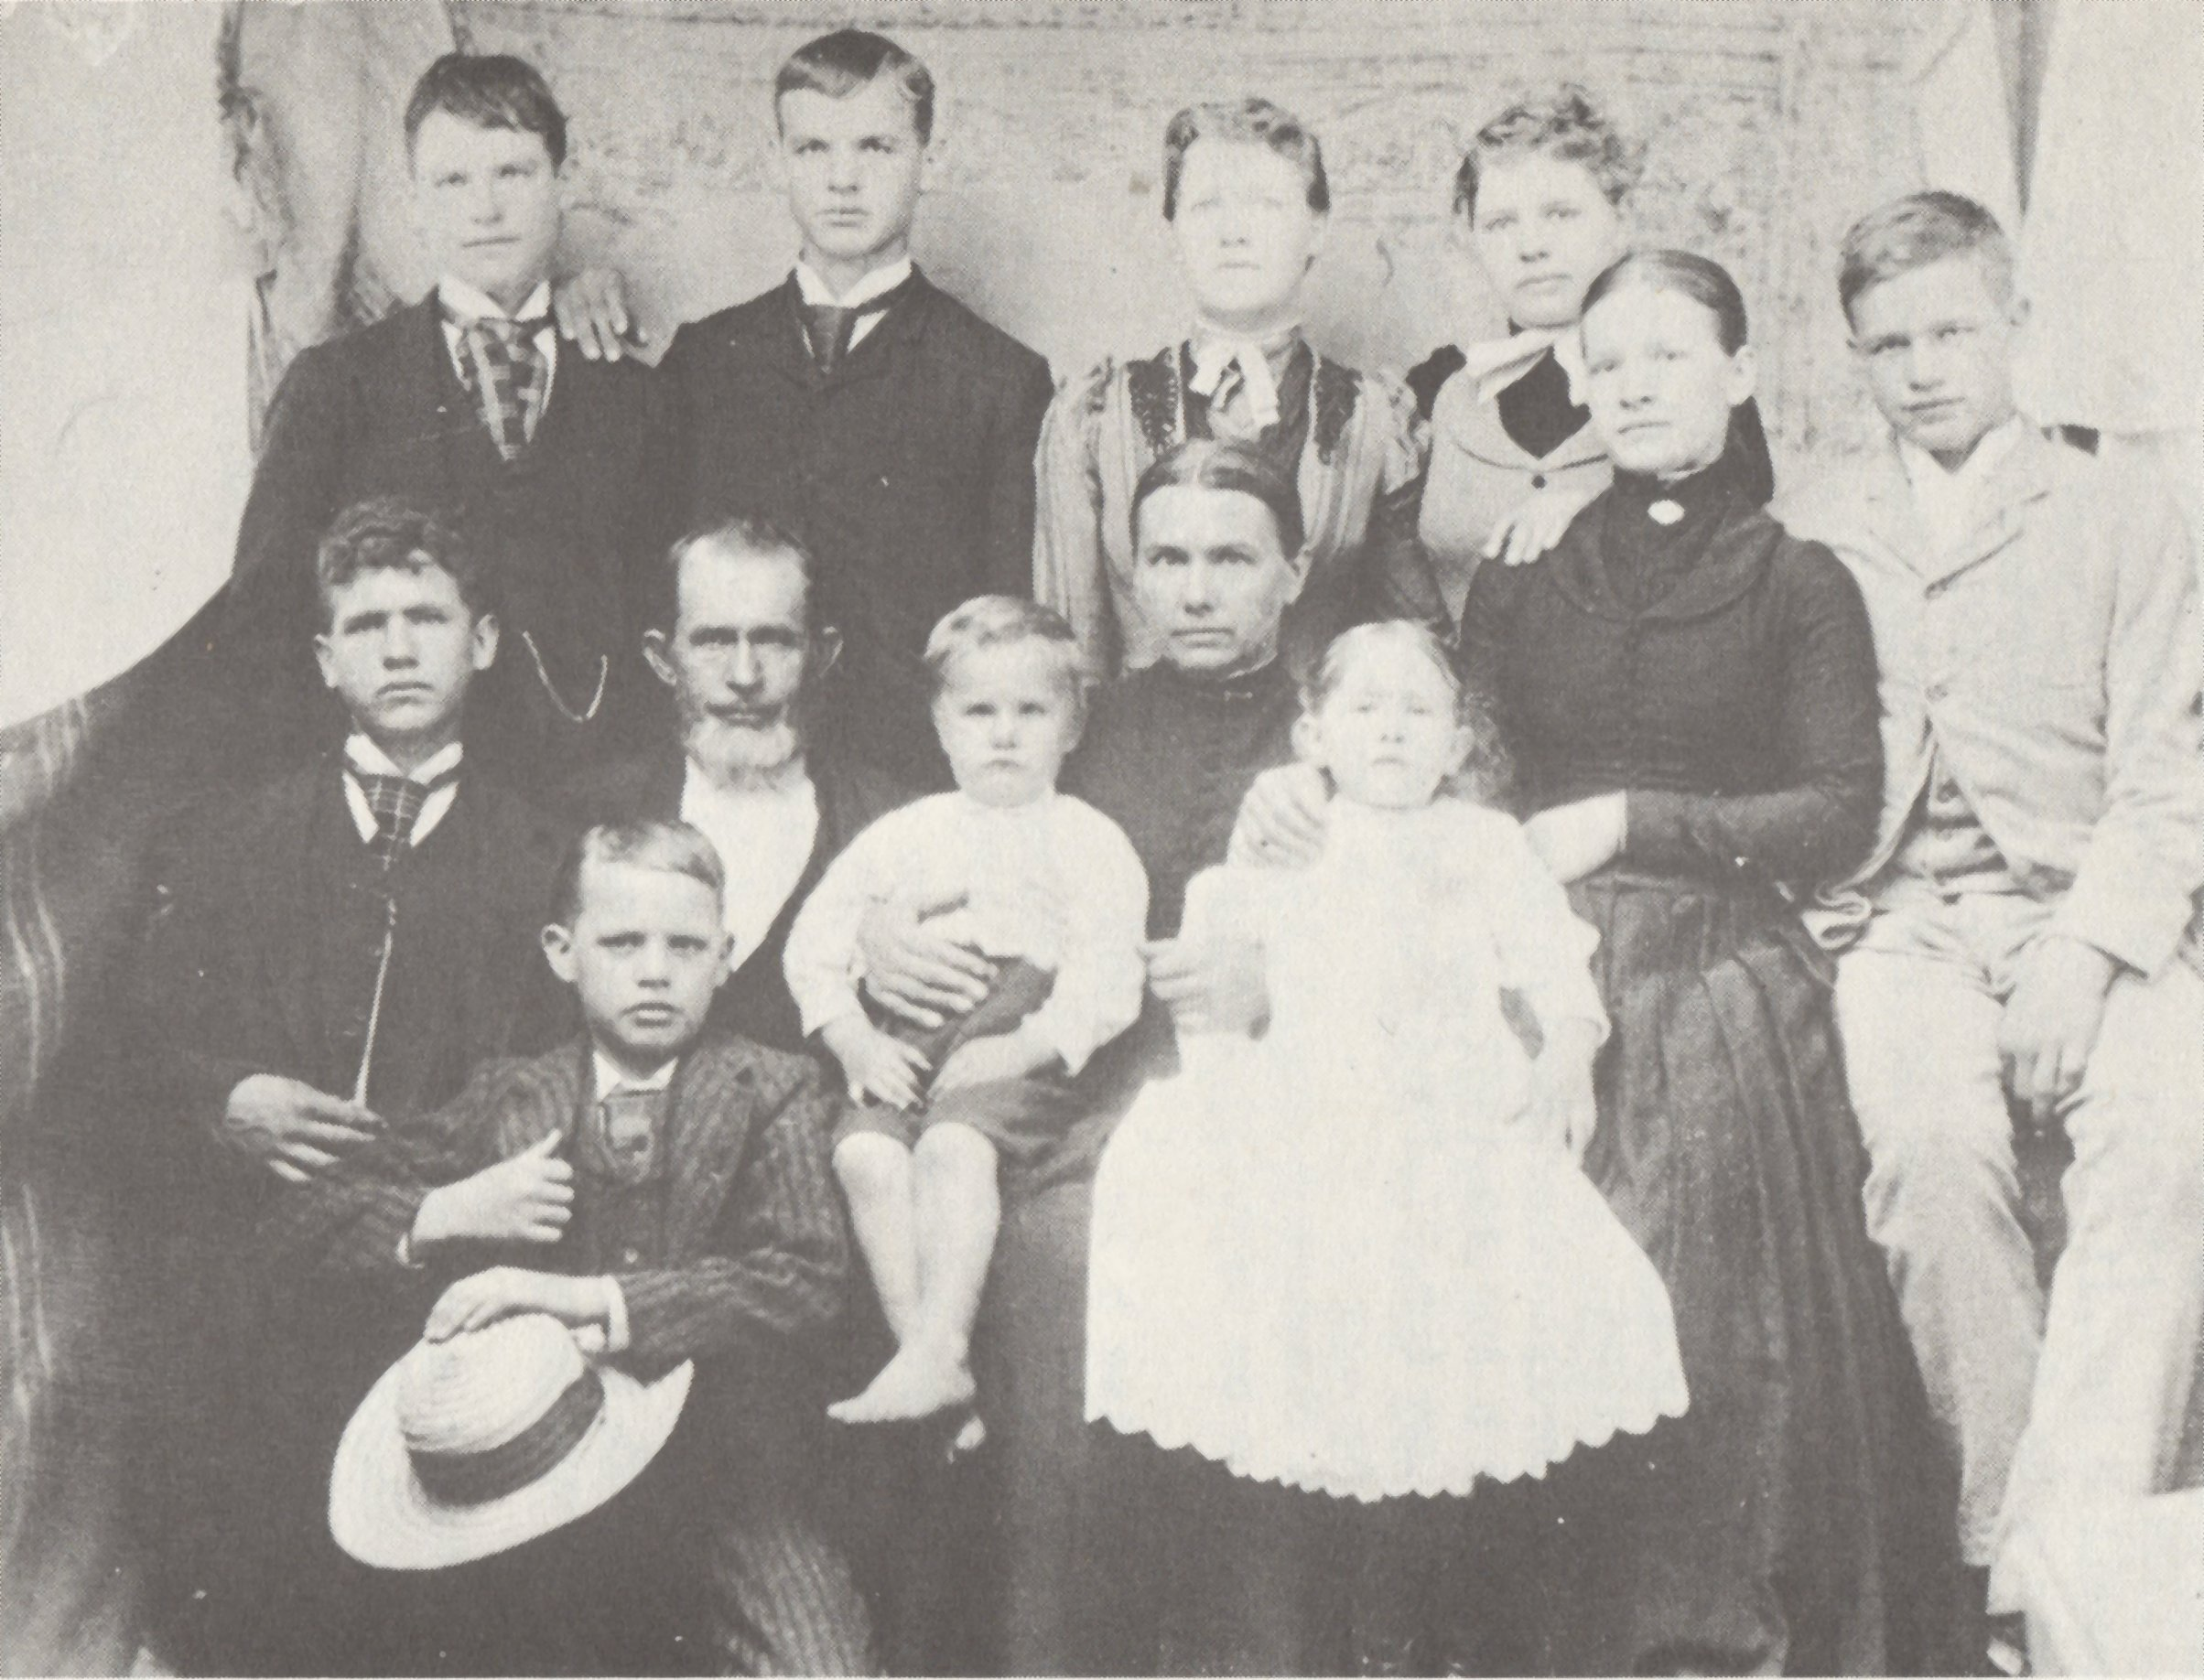
\includegraphics[width=1.0\textwidth]{family_photo.jpg}
\label{}
\end{figure}


%[Photograph of the family]

 
%********** End of chapter **********
